\chapter{Зверинец}

Некоторые воспоминания мои о Зверинце просочились в другие главы, здесь не буду повторять сказанное прежде.

Я жил на холмистом, зеленом да садовом Зверинце (мы называли его Печерском) с рождения в 1977-м, и по конец 1999-го. Мыслями возвращаюсь туда часто, а телесно в лучшем случае пару раз в год, на велике или метро. Доезжаю до станции «Дружбы Народов», поднимаюсь эскалатором и думаю, глядя на проносящихся мимо людей – а, я тоже здешний. И завидно, что они ходят по моему району каждый день, обыденно.

Помню, отправился туда летом 2012-го, с левого берега на правый, купив себе тогда дорожник «Аист» и навёрстывая упущенное с юности безвелосипедное время. В дурацком велошлеме, никем не узнанный, будто невидимка, я зарулил в родной двор – некогда просторный, а ныне полный машин. Кроме автомобилей, почти всё то же.

Береза у скамейки рядом с мусорником, темный гнилой деревянный стол для игры в домино, всё тот же пьяница Н-ко, ничуть не изменившийся за десятилетия. В восьмидесятые-девяностые была там компания пьяниц. Однажды они сбросили с балкона труп сотоварища. Тело упало на дорожку между домом и каменной подпорной стеной.

Пятиэтажка номер 11-А на Бастионной. Рядом стоит такая же хрущовка под номером 11, однако по адресу Бастионного переулка. Ниже 11-А – дом 13 снова на Бастионной, «Арсенальский», возведенный для рабочих этого завода. Наш же дом был смешанных ведомств, его строили в 1959-м сами арсенальцы (на «Арсенале» трудился дед Шурик), с «Полиграфкниги» (бабушка Таня работала там переплетчицей, а потом контролером), и наверное доковцы, с Дерево-обрабатывающего комбината. Раз они потом в нем жили, то наверное и строили. Кажется еще и с трикотажной фабрики.

Весной 2014-го я поехал на Лукьяновку проведать бабушку, которую выписали из больницы после второго инсульта, настигшего ее в 89 лет. Сидели на солнечном балконе и беседовали. Я спросил, как строился дом на Бастионной, что там было, и она рассказала, что сначала была «гора», которая оползала. Привезли огромные валуны, разбили их, и камнем выложили подпорную стену, что теперь отделяет пространство между домом и палисадником, который забором граничит с ботаническим садом. В 1960-х вместо забора был ров.

% – Там была гора. И эта гора была выложена камнями. И потом эту гору... Она начала сползать... И потом выбрали, прораб выбрал это место для стройки, и они разобрали эту гору, и получился котлован. И в этот котлован пошли эти камни. И вот это подкрепление, эту стенку укрепляли\footnote{Имеется в виду выложенная черным камнем подпорная стена за домом, между ним и горкой палисадника, переходящего в ботанический сад. Вместо ботсадовского забора в 1960-х там был ров.}. Вот, и поставили там дом.

   Арсенальский дом и 11-й возвели позже нашего. Строить 11-А бабушка ездила отработав смену на фабрике. Смешивала цемент, возила, выкладывала кирпичи. Звуковой файл передает мои вопросы и неторопливый бабушкин говорок.

 – А Арсенальский дом уже стоял тогда?

 – Нет. Арсенальский дом построили тогда, когда уже наш почти готов был.

 – А что было на месте Арсенальского?

 – А что было на месте Арсенальского – там был магазин, гастроном.

 – А рядом, где 11-й дом?

 – Не знаю, не помню.

 – А что-то ходило на Бастионную тогда из транспорта?

 – Ходил автобус сначала 62-й, потом уже провели троллейбус 14-й.

 – А как ты добиралась на работу?

 – Ехала 62-м до Бессарабки, а от Бессарабки ходил 9-й автобус, до Гарматной. Я ездила до Гарматной. На Гарматной выходила и, там немножко пройти.

 – А какой еще транспорт ходил у нас?

 – Тут ходил 16-й трамвай, с Печерска\footnote{Окрестности Печерского моста, Суворовского училища да и Бастионная считалась местными жителями Печерском. Троллейбусный же разворот находился напротив дома по бульвару Леси Украинки, 29.} и до площади Европейской. Потом, пустили троллейбус. 

Такой разговор.

Три хрущовки – 13, 11, 11-А – расположились за кинотеатром «Слава», о котором я еще подробно расскажу. В наш переулок (адресно поделенный между улицей и собственно переулком) – а это длинный уступ на склоне – от улицы заезд, обсаженный сиренью. Справа вырос кооперативный дом о девяти этажах, а раньше, в шестидесятые, там стоял частный дом трубача. Он выходил на крыльцо и играл на трубе. Мне мама рассказывала.

Чаще всего к дому 11-А ходили по Горке от Арсенальского дома:

\begin{center}
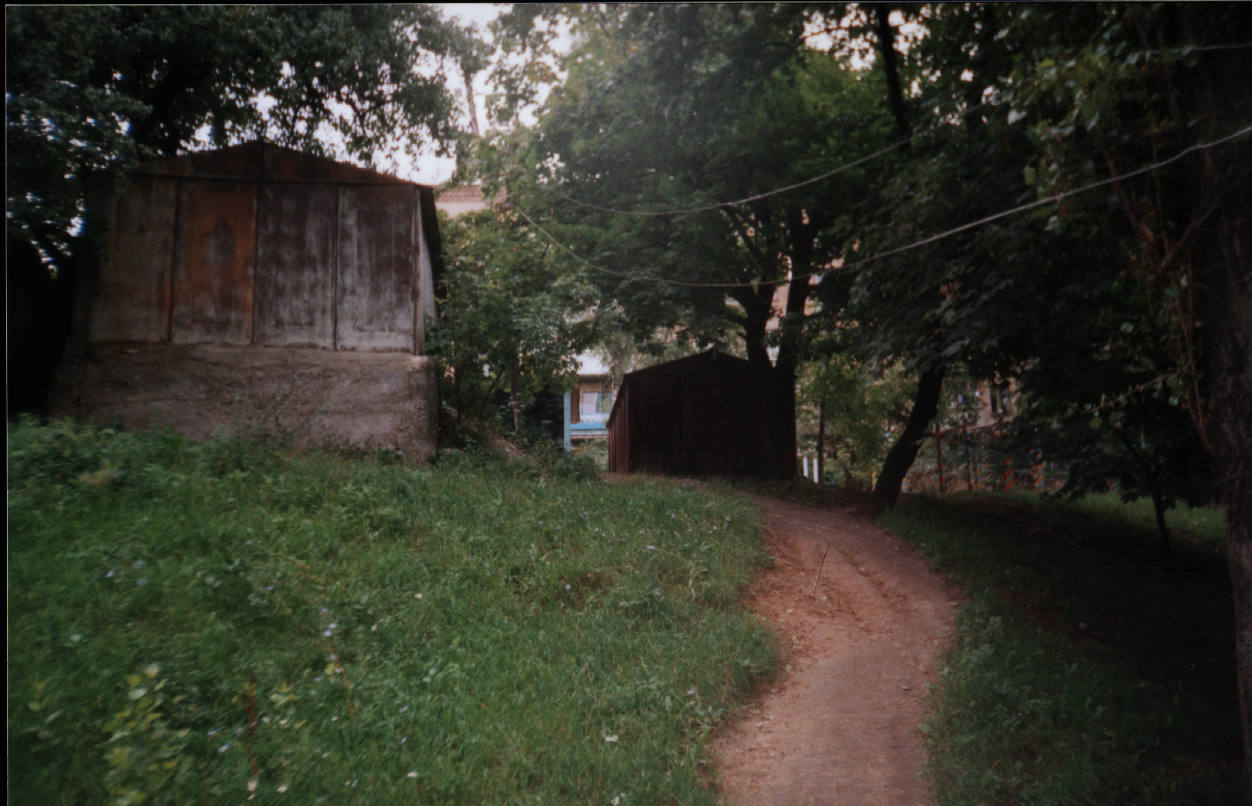
\includegraphics[width=\linewidth]{chast-vosp/zver/gorka.jpg}

\textit{Снимок 2003 года.}
\end{center}

Дом 11-А – первый по счету в переулке, стоит под горой, сам на небольшом пригорке, как бы постаменте. С тыльной стороны, на горе начинается ботанический сад, отделенный от придомового палисадника забором. А в постаменте спрятан подвал, где жильцы дома имеют каморки для хранения всяких овощей или барахла. 

%У нас такая появилась в девяностых, когда верхние соседи, Шимберги, уехали в США или Израиль, и отдали подвальную кладовку нам.

За домом – тишина и вечная тень. Зелень под ветром колышется. Асфальтовая дорожка и каменная стена, чтобы гора не оползала. Вдоль стены поверху бежит тропка, над нею обсаженный фруктовыми деревьями склон, выше еще одна тропка мимо забора ботанического сада. Выходит к площадке. Там, дождливой ночью, на яблоньке около стола, где на гитарах играли, пили и гуляли, повесили мужчину, и до утра несильно раскачиваясь, мокнул он под ливнем.

Каменная стена в приближении к дому 11 переходит в бетонную. Мы там играли и лазали, хотя было наверное опасно. Между блоками и суглинком шел заросший лозой зазор, там вечно лежали картонки, доски, здорово было прятаться.

Затем начинаются, между домом 11 и ботсадом, среди фруктовых деревьев, выкопанные в холме погреба. Их череда прерывается частной усадьбой, от которой на 2015-й остались развалины. Стоял глинобитный домик, почти хата, с сараем, цветником, аккуратной оградой да калиткой. В начале 90-х оттуда съехали жильцы, среди них бледный мальчик Тарас, мы иногда играли в ножички, войну, и как-то нашли в земле у цветника покореженную гильзу 1913 года.

Затем снова идут погреба и бугрится высоко местность Собачка, о ней я поведал в начале книги.

А перед 11-А обычный двор, две скамейки, детская площадка, мусорник и дальше, у Горки – возле груши-дички несколько ржавых гаражей, по ним было здорово бегать, под ногами гудели. От детской площадки спускался крутой склон в Арсенальский двор.

Как-то зимой прорвало водопровод и вода залила этот склон до самого низа. Сплошной лед! Это же какая будет скорость, если на санках! Сел, поехал. Не успел сообразить, что рулить-тормозить не получается. Видел только, как неумолимо несёт к толстенному клёну, там еще деревянный брус к его стволу тросом прикручен. Привет!

Я долбанулся передом санок в брус, меня бросило дальше и левее. Время замедлилось. Санки сами по себе летят в одну сторону, я в другую, мир вращается. Вот наконец падаю. Плотный наст. У меня шапка-ушанка сбита на лицо. Думаю – ааа, голову себе проломил, всё, там вмятина в черепе. Да вроде нет. Не знаю. Одурело подобрал санки, погнувшиеся в поперечном бампере. Полез наверх, по снежку. Дома оклемался.

На детской площадке я обычно игрался один, любил качаться на качелях под сгорбленной марелькой. Туда-сюда, и если сильный размах, то можно ногами захватиться за ветку и удержаться. Марельку посадила старушка, известная мне как «баба Фаня», хотя её звали вовсе не Фаня, и кажется, никто кроме меня её под этим именем не знал. У нее была внучка Алёна. Мы потом купили у этой бабы Фани внучкин велосипед, складной «Минск». Я стал уверять всех, что весит он сто килограммов, и прокатался на нем много лет, пока не вырос.

Из аттракционов на площадке первой помню деревянную низенькую горку, при ней я совсем еще малой был. Затем поставили новые забавы, металлические – вот эти качели, карусель, большую двухэтажную горку в виде ракеты, дугу с поручнями и деревянного, обитого железными листами, крокодила.

Карусель представляла собой сиденья, вращавшиеся вокруг оси с круглым рулем, за который надлежало хвататься и крутиться. Руль быстро поломался, но мы катались, отталкиваясь ногой от земли. Постепенно карусель пришла в полный упадок – остался лишь стальной, причем вполне подвижный каркас.

А горка-ракета почти доставала острой верхушкой до ветвей высоких кленов, и к ней дотягивалась космами большая ива. Я играл в космические полеты, проходя последовательно все воображаемые этапы. Перед запуском проверял запас топлива, потом стоял у трапа, прощаясь с провожающими. Поднимался, взлетал. Если что-то шло не так, шатал ракету руками и сам же откликался – ааа, мы потеряли управление! Вылезал на верхушку или к дюзам, чинил поломку. Затем ложился курсом на орбиту либо отправлялся на другую планету – ее поверхностью служила вся детская площадка. Я съезжал с гулкой, блистающей горки и начинал исследовать диковинную местность, готовый в любую секунду смыться назад на ракету от враждебных роботов.

Справа от площадки, через скамейку и березу, был мусорник. Сарай с окошком, туда опорожнялись вёдра. Контейнеры для мусора появились к концу девяностых, купно с первыми бомжами. Поначалу воспринималось невероятно, что человек ищет еду в мусоре. Оттуда, и дальше ко двору дома 11, уцелел осколок частного сектора – несколько дворов – до здания ПТУ и кинотеатра. Каждое утро кричал петух.

Двор дома 11 осенью усыпа\'ли орехи, росшие над ним. Позади номера 11 палисадника не было (кроме как от хибары Тараса), но был перед, ухоженный, с деревянным заборчиком. Как приходила пора, весь асфальт усеивали орехи, яблоки. После развала Союза и кое-что другое. В одной квартире, на кухне, взорвали директора какой-то фабрики, и по двору валялись алые кусочки костей с мясом и слипшимися волосами.

\vspace*{\fill}
\begin{center}
\includegraphics[width=\linewidth]{chast-vosp/zver/\myimgprefix IMG_20130826_173138.jpg}
\textit{2013 год. Заезд к домам 11, 11-А, 15. Слева – Арсенальский дом.}
\end{center}
\vspace*{\fill}
\newpage

\begin{center}
\includegraphics[width=\linewidth]{chast-vosp/zver/\myimgprefix DSC_0029.JPG}

\textit{2012 год. Вид оттуда вниз.}
\end{center}

\begin{center}
\includegraphics[width=\linewidth]{chast-vosp/zver/\myimgprefix DSC_0030.JPG}

\textit{2012 год. И вверх, в сторону ботсада.}
\end{center}

\newpage

\begin{center}
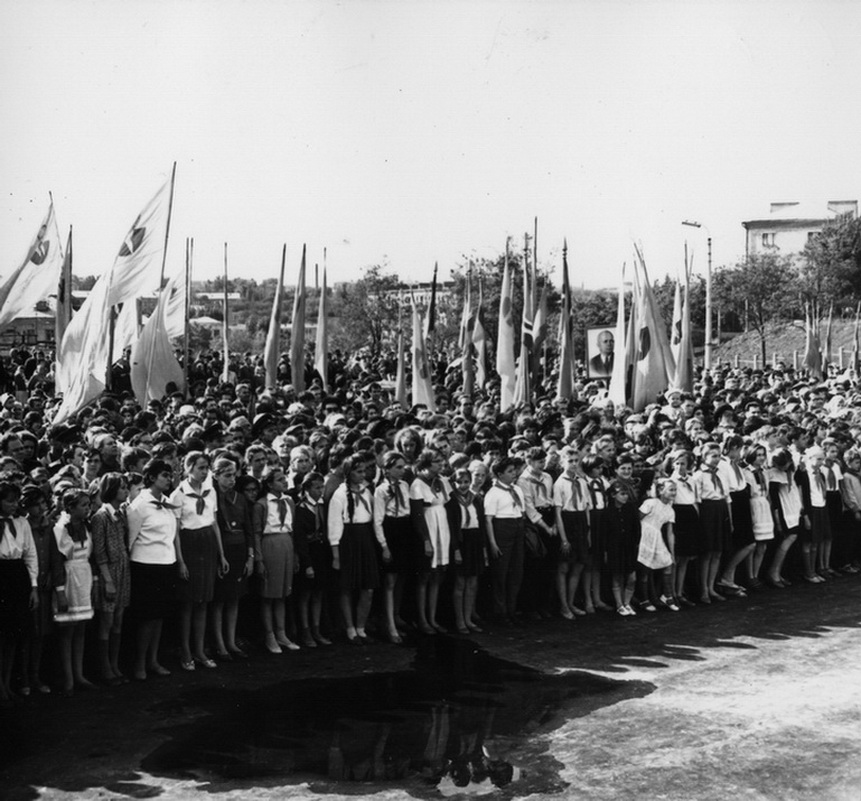
\includegraphics[width=\linewidth]{chast-vosp/zver/1964-botsad.jpg}

\textit{29 мая 1964. Митинг по случаю открытия ботсада. Снято от площади у его входа. Справа виден дом 11-А, еще не заслоненный белой высоткой.}
\end{center}

\begin{center}
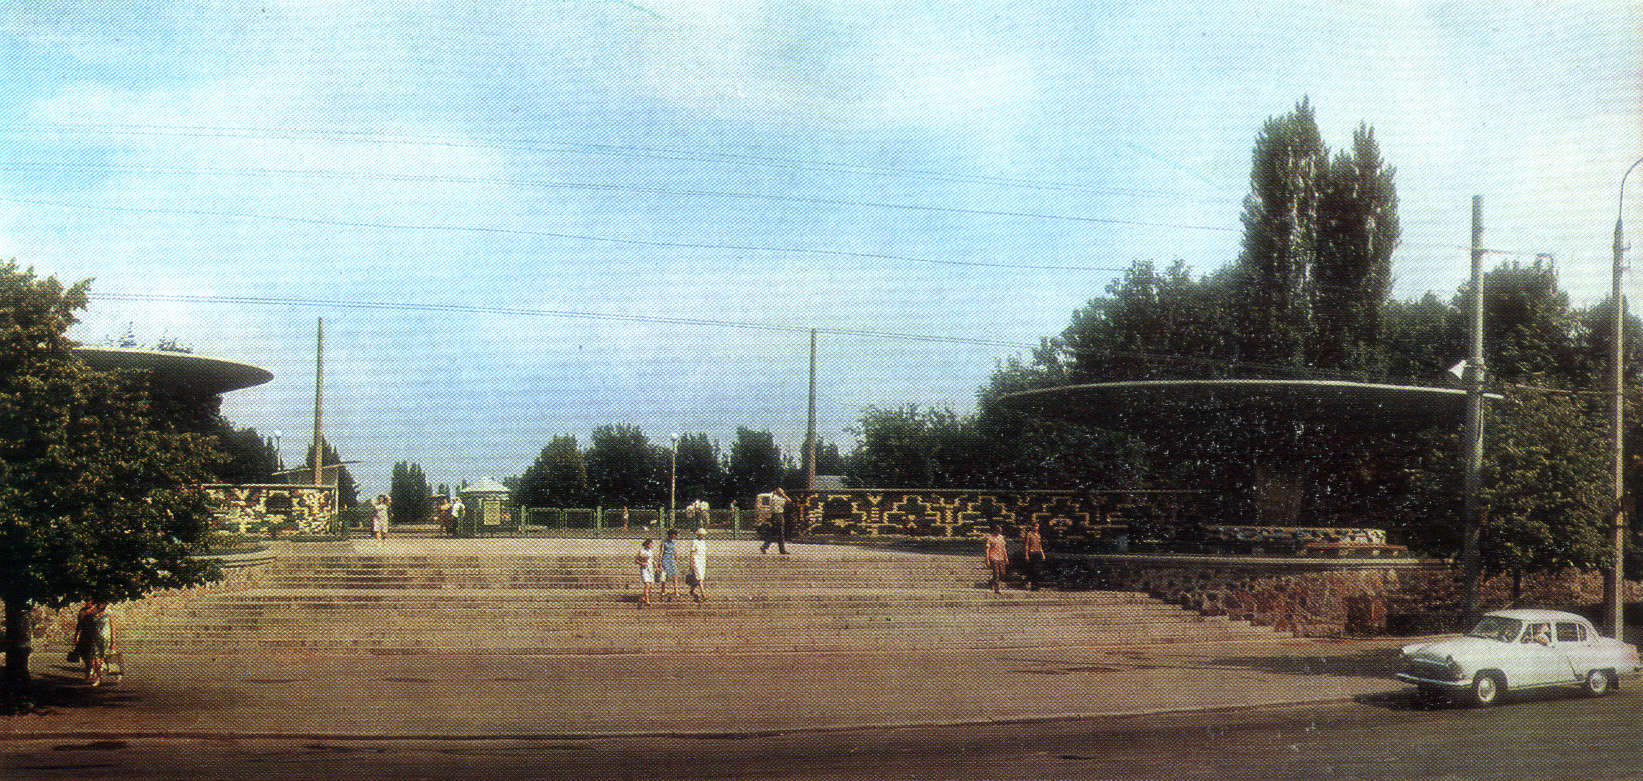
\includegraphics[width=\linewidth]{chast-vosp/zver/1974-botsad.jpg}

\textit{1974. Вход в ботсад.}
\end{center}

\begin{center}
\includegraphics[width=\linewidth]{chast-vosp/zver/\myimgprefix DSC_0033.JPG}

\textit{2012 год. Вид со двора дома 11 на двор и дом 11-А.}
\end{center}

Вот первое отсюда парадное – моё. Справа – частные дома, уцелевший уголок, их на снимке не видно. Моего окна тоже, оно левее. Во глубине кадра – белая высотка – это дом 15, на пригорке, где некогда в частной усадьбе жил трубач.  

\newpage

\begin{center}
\includegraphics[width=\linewidth]{chast-vosp/zver/\myimgprefix DSC_0032.JPG}

\textit{2012 год. Вид со двора дома 11-А на двор и дом 11.}
\end{center}

Слева – поворот к мусорнику. Впереди за хрущовкой 11 белеет Дом Художников (Бастионный переулок, 9). Бастионный переулок отходит от узенькой улицы Струтинского (Болсуновской) и по уступам заползает сюда.

\newpage

\begin{center}
\includegraphics[width=\linewidth]{chast-vosp/zver/\myimgprefix DSC_0034.JPG}

\textit{2012 год. За домом 11-А.}
\end{center}

Слева – мой прежний дом, справа – знаменитая подпорная стена и палисадник. Дальний балкон на 4-м этаже, оттуда я смотрел на шумящую чащу деревьев, дышал запахом сирени и цветущих вишень. Это сейчас его застеклили, а у нас был просто обитый клеенкой дощатый каркас. В глубине кадра, с пересветом, 11-й дом.

\newpage

\begin{center}
\includegraphics[width=\linewidth]{chast-vosp/zver/\myimgprefix DSC_0036.JPG}

\textit{2012 год. За домом 11, вид в сторону Собачки.}
\end{center}

А это за домом 11. Сколько раз я тут, катаясь по кругу, проезжал на велике! Справа ступенечки ведут к погребам в склоне холма, а еще дальше и справа -отсюда не видно – развалины частного дома.

\newpage

\begin{center}
\includegraphics[width=0.99\linewidth]{chast-vosp/zver/\myimgprefix DSC_0038.JPG}

\textit{2012 год. Там же, но вид в обратную сторону. Слева палисадник от частного домика.}
\end{center}

\begin{center}
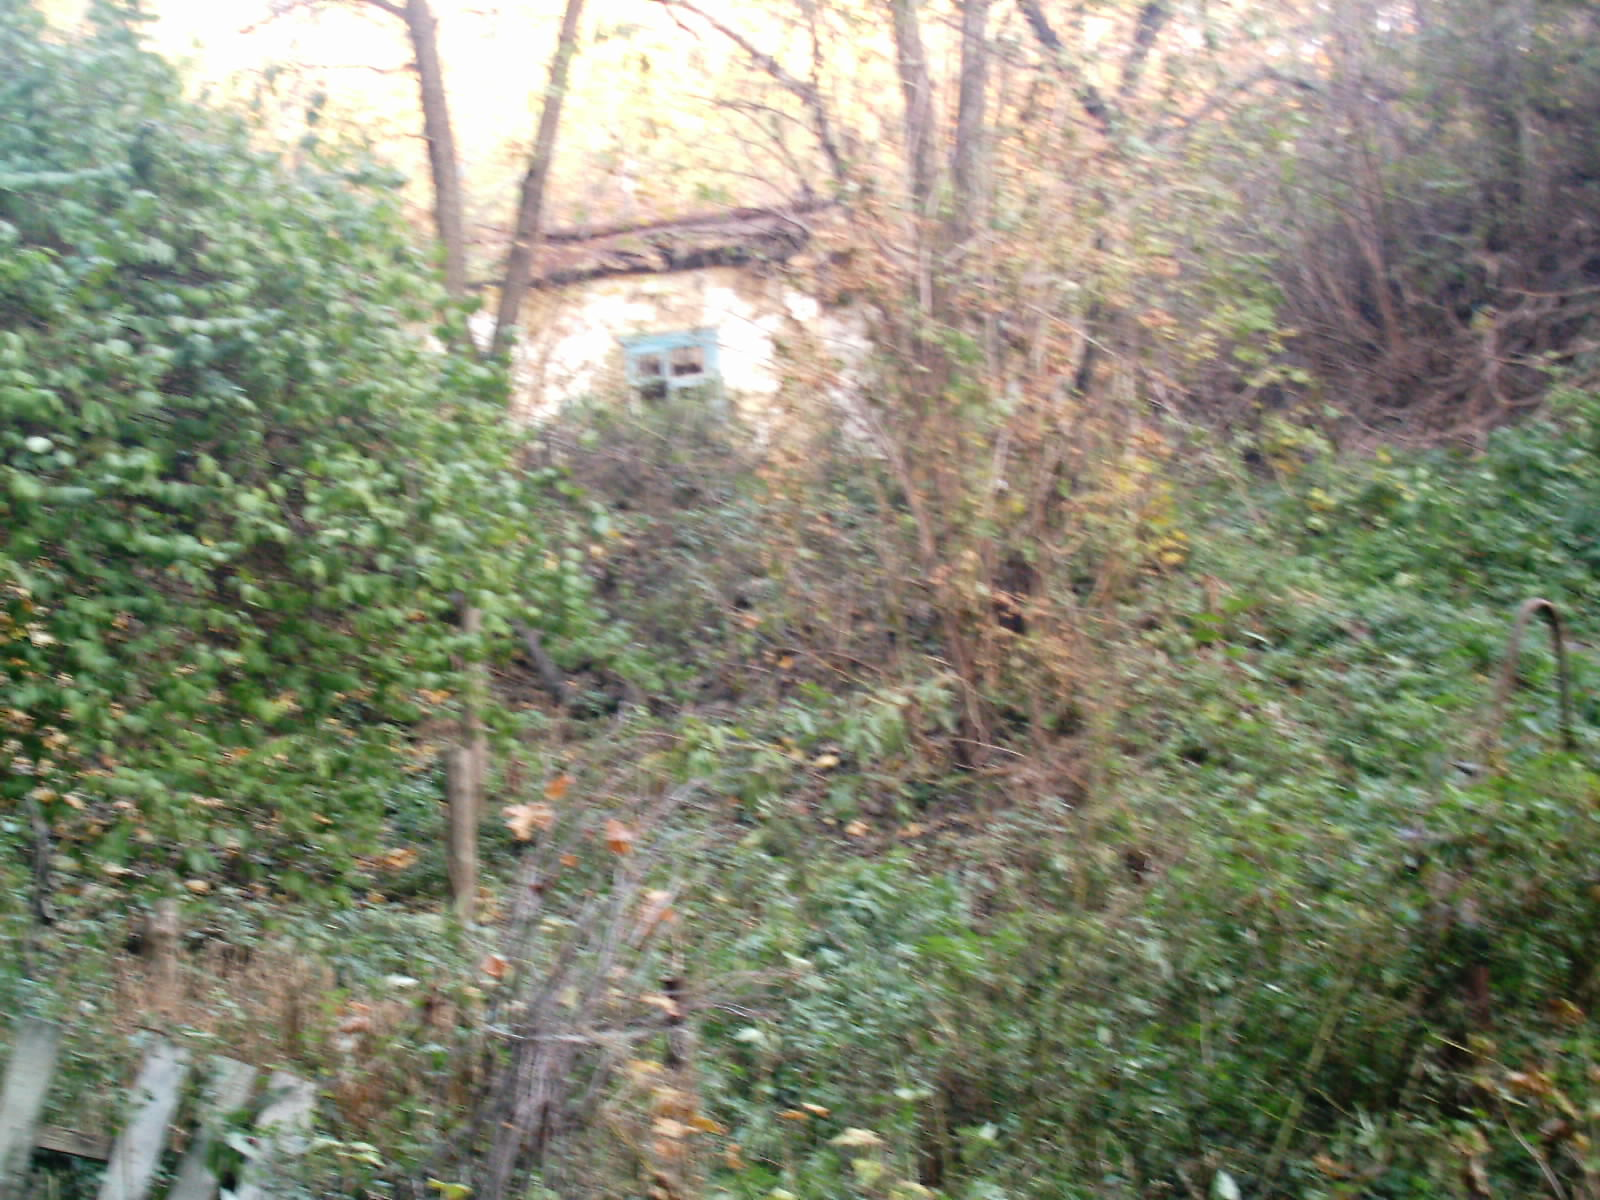
\includegraphics[width=0.99\linewidth]{chast-vosp/zver/imag0036.jpg}

\textit{2005 год. Развалины того частного домика.}
\end{center}

\newpage

Ну и вот, дальше шла Собачка, рядом с ней в глубоком овраге – Дом художников, где жили люди искусства, и потом улица Мичурина, бывшая Ломаковская, там у нас родственники, а дом их стоит еще с довоенных лет. Это про него Кузнецов в «Бабьем яру» писал: «На Зверинце жила тетя Оля с мужем. Они работали на «Арсенале» и эвакуировались с ним. Перед  самой  войной они построили  домик на Зверинце». 

Я же знал «тетю Олю» из романа уже как «бабу Олю», она умерла в 1993 году. Не раз бывал в том домике. А на его чердаке  обитал домовой.

До строительства в 1950-х, от нынешнего перекрестка Бастионной, Струтинского, Билокур, под углом к Бастионной отделялась грунтовая прямая дорога, что шла по нынешнему ПТУ, за кинотеатром Славой (к северу), частной усадьбой, затем между будущими домами 11 и 11-А, и далее в ботсад. Сейчас если свернуть между домами, то справа от бетонной части подпорной стены – заход в небольшое удолье, овражек с погребами по обоим берегам. В нем-то и проходила дорога. В ботсаду она достигала точнехонько юго-западного угла остатков Зверинецкого форта.

\begin{center}
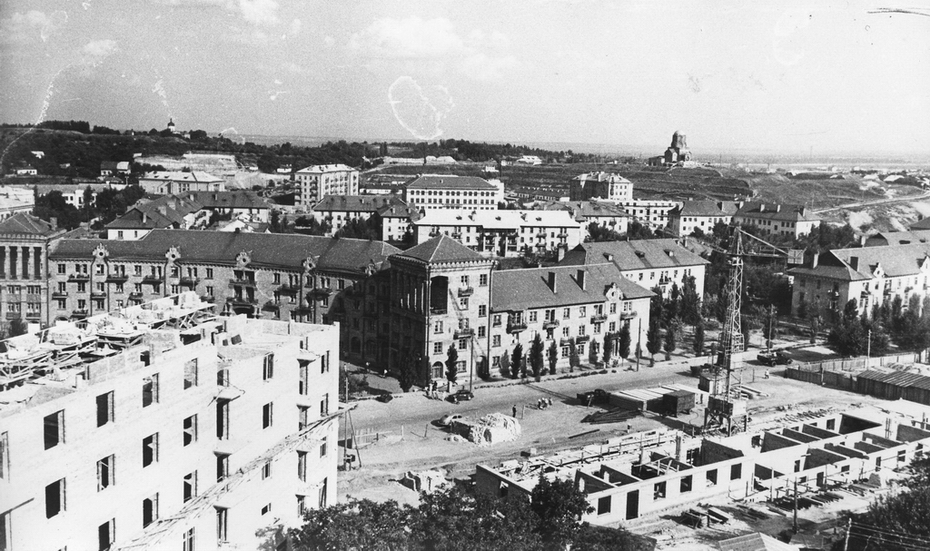
\includegraphics[width=\linewidth]{chast-vosp/zver/0932_KK.jpg}
\end{center}

На снимке выше, 1958 года, виден еще пустой суглинок пригорка, кажется раскопанного, над кинотеатром «Слава», где вскоре возведут дома 11, 11-А, а ниже, почти вровень со «Славой» – 13-й Арсенальский.

Церковь на горизонте, в левой части фотографии – Ионинский Свято-Троицкий монастырь. Переведите взгляд чуть ниже – светлый искомый пригорок. Еще ниже – кинотеатр. Церковь справа и террасы – это Братское кладбище для солдат, погибших в Первую мировую, да Никольская церковь при нем. Ныне там Институт проблем прочности, а бывшее здание церкви один из его корпусов.

На переднем плане полукругом стоит дом 2/1, построенный в 1952 году. Перед ним – «Пятачок», он же «Яма». Называется так потому, что напротив него склон холма (на снимке не видно), тоже полукругом, и в удолье образуется эдакий пятачок.

Существует путаница. Для жителей Мичурина, и домов около Бастионной 11-А, Ямой слыла в самом деле глубокая яма, где под склоном горы стоят дома Бастионная 12 и 14. Обитатели же, кажется, начальных номеров Бастионной, Ямой называют то, что мы именовали Пятачком.

«Пятачок» также и собирательное название почти всего просторного внутри квартала, который строился, кажется, пленными немцами и от полукруглого дома расходится с одной стороны вдоль Бастионной, с другой – Киквидзе, и ограничивается улицами Подвысоцкого и Катерины Билокур (ранее Евгении Бош). Там жилые, большей частью трехэтажные, дома стоят по периметру, а внутри заключаются пустыри, детская площадка, бомбоубежище, детский сад и поликлиника. На Пятачок за домом с аркой мы ходили часто, в магазины и на базарчик. Сначала на нем стояли грубой работы деревянные столы-прилавки, затем появились моднее, с навесами. Там продавалась зелень, картошка, семечки, соленые огурцы, сухая фасоль.

Сейчас базарчик сохранился и расширился, а вот магазины почти все изменили назначение. Да исчез ларек с квасом! Помимо кваса, в той части Пятачка, что ближе к Бастионной, была наливайка, куда, кроме забулдыг со всех окрестностей, нередко захаживал известный советский актер. За нею, в склоне, соорудили общественный туалет. Рядом наверх вела каменная лестница с кривыми ступенями, сверху разбит сквер, в нем по нулевые оставались деревянные столбы электропередач.

Если сойти с лестницы и глядеть прямо на полукруглый дом с аркой, сквозь рынок, то магазины в восьмидесятых годах (в 1950-х там располагались еще столовая и телефонный узел) на первом этаже были, слева направо, следующие.

«Галантерея» со всякими нитками, иголками, парфюмерией, лентами. «Хлеб», очень чистый и светлый магазин с самообслуживанием и кассой в конце отгороженного коридорчика, в котором и брался с полочек хлеб. Особенно вкусной была пшеничная, с полукруглым наростом над основной буханкой, «Паляныця». На стене там висел плакат со стихотворением:

\settowidth{\versewidth}{Хлеб – не просто дар природы,}
\begin{verse}[\versewidth]
Хлеб – не просто дар природы,\\
Хлеб – наш труд, не забывай!\\
Береги же наш народный,\\
Драгоценный каравай!
\end{verse}

Я хорошо его запомнил, ибо часто видел. Кроме паляныци, мы покупали обычно черный «Украинский» хлеб и булочки. Я любил соленый «Рогалик закарпатский» по 6 копеек штука, и маленькие булочки по 3 копейки, сейчас их выпускают в пачках под названием «Малятко». Были еще очень вкусные диетические хлебцы, похожие на «Кирпичик», но меньше. Еще в «Хлебном» на полках лежала мука, крупы и макароны.

Дальше арка. Справа от арки – «Кулинария» с разными полуфабрикатами вроде дрожжевого, слоеного теста, котлетами да пирожными. Мне нравились полосатые «уголки» по 15 копеек. Там чередовались слои с какао и обычные. А между ними повидло. Иногда мы покупали тесто, дома я лепил из него круглые пончики, а мама жарила их на сковородке.

%Однажды я, тоже ребенком, вздумал делать варенье из лепестков роз. В розарии ботсада, набрал с роз лепестков и без всякого рецепта стал варить их в воде, набросав туда вволю сахару. Когда немного покипело, квартиру заполонил сладковатый дух, вызывавший тошноту. Я сразу выключил конфорку, вылил в раковину получившуюся жижу и на всю жизнь получил нетерпимость к запаху роз.

За «Кулинарией» был обычный гастроном. Всплывает в памяти, что кладу в кулёк бутылку с «Пепси», а поскольку ростом еще мал, то дно кулька на уровне пола, и бутылка разбилась. Из заграничных вод продавалась по лицензии «Пепси» и «Фанта».

Итак, это всё было на нижнем этаже дома с аркой, который внутри подобен дворцу своими высоченными потолками и громадными коридорами, а так это общежитие.

Напротив гастронома будто в землю врос коренастый, одноэтажный магазин с мясом, рыбой и молоком. С краю от него, ближе к базару – киоск с квасом. Были такие, вроде грибов, и на шляпке большие буквы: «КВАС». В отличие от перевозных бочек, исчезавших с холодами, эти киоски стояли круглый год, но работали тоже в тепло. Чтобы квас лился, для вытеснения его из емкости подключался баллон со сжиженным углекислым газом. Квасная же бочка лишена баллона, там кран торчит внизу, всё само льется.


\begin{center}
\includegraphics[width=\linewidth]{chast-vosp/zver/\myimgprefix IMG_20130826_173616.jpg}

\textit{2013 год. Внутри Пятачка. Впереди – дом с аркой.}
\end{center}

С тыльной стороны дома с аркой, в подвальчике, находился пункт зарядки сифонов, туда выстраивалась очередь. Было такое дело – сифоны заряжать. Большой, на два-три литра сосуд с краном и рычагом наверху, заряжался сладкой газировкой. Нажимаешь рычаг – в стакан льется лимонад. Сиропы – на выбор. Или просто с пузырями. И вот мы с верха Бастионной ходили с этими сифонами на Пятачок и тащили их обратно, уже наполненные. Потом пункт зарядки прикрыли, оставался еще один в Гидропарке, мы ездили туда по крайней мере единожды с этой целью. В подвале же, кроме сифонов, заряжали еще чернилами стержни для авторучек.

Рядом, насколько я помню, принимали пустые бутылки.

Вообще Пятачок довольно удивителен, ибо жилыми домами образует как бы толcтую стену, ограждающую внутреннее, разреженное пространство – много узких дорожек – грунтовых либо выложенных бетонными плитами. И пустыри, пустыри под деревьями.
 
Внутри и вокруг квартала я часто катался на велике, то сам, то с пацанами со двора. 

В угловом доме на улице Билокур, возле перекрестка напротив 133-й школы, с одной стороны была почта, с другой книжный магазин. Почта существует поныне, а книжный сначала преобразовали в стрип-клуб, а потом во что-то еще. Вход в книжный сторожила скрипучая, на тяжкой пружине, дверь. Внутри всегда прохладно и пахло не бумагой, а лаком для мебели, что ли? Как войдешь, там направо, за кассой приютился букинистический отдел, в его развалах я рылся более, чем обращал внимание на новые книги.

Помню, что взял там две книги Роберта Мерля – «Мальвилль» и «Животное, наделенное разумом» (последнюю так и не прочитал), несколько брошюрных томиков серии «Литературные памятники» – «Фламандские легенды» Шарля де Костера с ужасной сказкой о Сире Галевине и каменном человечке, «Сага о Серги и Абенсераххах», и Томаса Лав Пикока (не осилил), зачитанный до дыр «Кортик» Рыбакова, самиздатовское «Собачье сердце» в синей «обложке работы Ю. П. Анненкова», как гласила надпись. 

В этом же книжном я стал собирать книги Салтыкова-Щедрина, которого открыл для себя в школе рассказом «Как один мужик двух генералов прокормил». Приобрел и «Сказания русского народа» Сахарова – с чего началось мое ранее увлечение народным творчеством.

\begin{center}
\includegraphics[width=\linewidth]{chast-vosp/zver/\myimgprefix IMG_20130826_173500.jpg}

\textit{2013 год. Дом с почтой и уже без книжного.}
\end{center}

Через проход от букинистического отдела, в шкафу стояли книги на обмен – разные ценимые издания, кои можно было обменять на подобные. Сейчас ими забиты коробки с макулатурой на Петровке – Майн Рид, Буссенар, Пикуль, Фрейд. А когда началась Перестройка и появились разные кооперативные книги, их выставляли на продажу в том же шкафу, втридорога. Серии про Тарзана и прочее – ныне они занимают то же «почетное» место на Петровке, что и Майн Рид. А выменять «Всадника без головы» было ого-го! Издательство «Мир» замечательную серию про животных издавала, помню Даррелла мы выменяли, «Мою семью и других зверей».

%Напротив книжного – моя школа, номер 133, трехэтажная, построенная в 1936 году (вероятно, на месте дореволюционной лаврской школы, при которой был и сад). Во время Великой Отечественной войны немцы устроили в ней конюшню. При мне возвели второй корпус, а раньше на его месте были плодовый сад и небольшой стадион с дощатыми бортами. Зимой его заливали водой, устраивали каток. Туда ходили с коньками со всей округи. Тем, кто просто катался, сильно мешали отчаянные хоккеисты.

Напротив книжного – моя школа, номер 133, трехэтажная, построенная в 1936 году. Во время Великой Отечественной войны немцы устроили в ней конюшню. При мне возвели второй корпус, а раньше на его месте были плодовый сад и небольшой стадион с дощатыми бортами. Зимой его заливали водой, устраивали каток. Туда ходили с коньками со всей округи. Тем, кто просто катался, сильно мешали отчаянные хоккеисты.


А напротив сада, через улицу, на другой стороне Струтинского, за заборами виднелось несколько приземистых хат – потом их снесли в пользу новых зданий близлежащего ПТУ. Арсенальский рабочий Струтинский, чьим именем была переменовли улицу Болсуновскую, похоронен на крутогорбом Зверинецком кладбище, подъем на которое – прямо внизу этой улицы, на бульваре Дружбы Народов.

Окрестности перекрестка Бастионной, Бастионного переулка и улицы Струтинского в середине 19 века слыли Солдатской слободкой.

Заточенная в овраге от поворота к улице Мичурина, что резко сворачивает в сторону вверх, Струтинского сильно преобразилась еще во время, когда я жил на Бастионной. Выстроили эти новые корпуса школы и ПТУ, затем какой-то институт слева. Дольше продержался низ улицы, сейчас там здоровенные здания. А прежде на четной стороне в удолье, примыкая к холму с улицей Кургановской, приютилась частная усадьба – домик с приличным по размеру садом. В запустении она простояла, наверное, лет десять.

Рядом, однако по нечетной стороне, в низком домике, в советское время работала автомастерская, за ней, еще через усадьбу (ныне снесена, там автозаправка), наверх к переулку Мичурина карабкалась лестница с бетонными ступенями, и дальше она же вела к повороту улицы Мичурина, где двор со Зверинецкими пещерами. При мне в них стали ходить ближе к концу 1990-х, и то сверху, через дыру в заборе ботсада. А так был обыкновенный домик с участком.

Но вернусь к школе. Моя дорога туда вспоминается не иначе как мимо цветущих вишен и свежевыкрашенной в зеленый цвет, копейного образа, ограды ПТУ. В районе было три школы – моя №133, неподалеку, на другой улице – №88 (построена к декабрю 1953 году), и внизу Тимирязевской, на пригорке – пятая школа, с самолетом МИГ-17 на постаменте. Некогда окруженная частными домами, теперь эта школа соседствует с элитными новостройками, а напротив нее, в овраге за забором ботсада, протекает ручей Омелютинка. Над нею, сверху, на круче суглинного склона светлеет площадка, где растут стройные, с рыжими стволами, сосны. Старожилы называют этот склон горой Караваевкой, от местности Караваевщины.

Пятая школа с другой своей стороны выходит на улицу Бусловскую, потому что гора сия, зажатая между улицами Тимирязевской и Киквидзе, именуется Бусовой или Бусловой. Ниже лежит Бусово поле, и западнее, в коллекторе вдоль улицы Киквидзе, течет речка Бусловка, где в 19 веке водовозы со всего города набирали вкусную воду.

Бусловка названа, вероятно, по птице – у нас и в Беларуси «буслами» кличут аистов. Еще было слово «буслай» – гуляка, мот. Бусом также называли пыль. Буква «л» в источниках появляется да исчезает, и неясно, каков же корень – Бус или Бусел. А может и «буз». Буз, бузок – значит сирень.

А параллельно Бусловской улице идет Зверинецкая, еще одна магистраль Зверинца. Обе улицы, проложенные некогда по частному сектору, теперь застраиваются небоскребами и странными домами, напоминающими хранилища золотых запасов и средневековые замки.

От гастронома в доме на Зверинецкой, 63, и до Печерского моста, коротким маршрутом ходил автобусик, из тех, что можно было встретить в сельской местности или какими предприятия возили людей на ведомственные базы отдыха. Он вёз сначала к разворотному кольцу возле главного входа в ботсад, и дальше чесал по прямой, по Бастионной, до остановки за Печерским мостом, где поворот к военкомату. Улица Каменева, вот. Там же была и конечная трамвая, от центра, а до революции трамвайная ветка доходила в ботанический сад, к нынешнему перекрестку перед спуском сиреневой аллеи. Я нарочно пешком гулял к остановке автобусика, чтобы прокатиться на нем и пешком же вернуться домой.

Классический Зверинец по улицам Ольшанской (названа от живших тут в 19 веке Ольшевских), Дубенской, Зверинецкой, Тимирязевской, короче говоря всем, что примыкали к ботсаду, был знаком мне не теперешними теремами, а раскинувшейся по склону тонкой сетью узеньких проулков и лесенок среди гнилых заборов, через которые лезла зелень садов и белели домики. 

\begin{center}
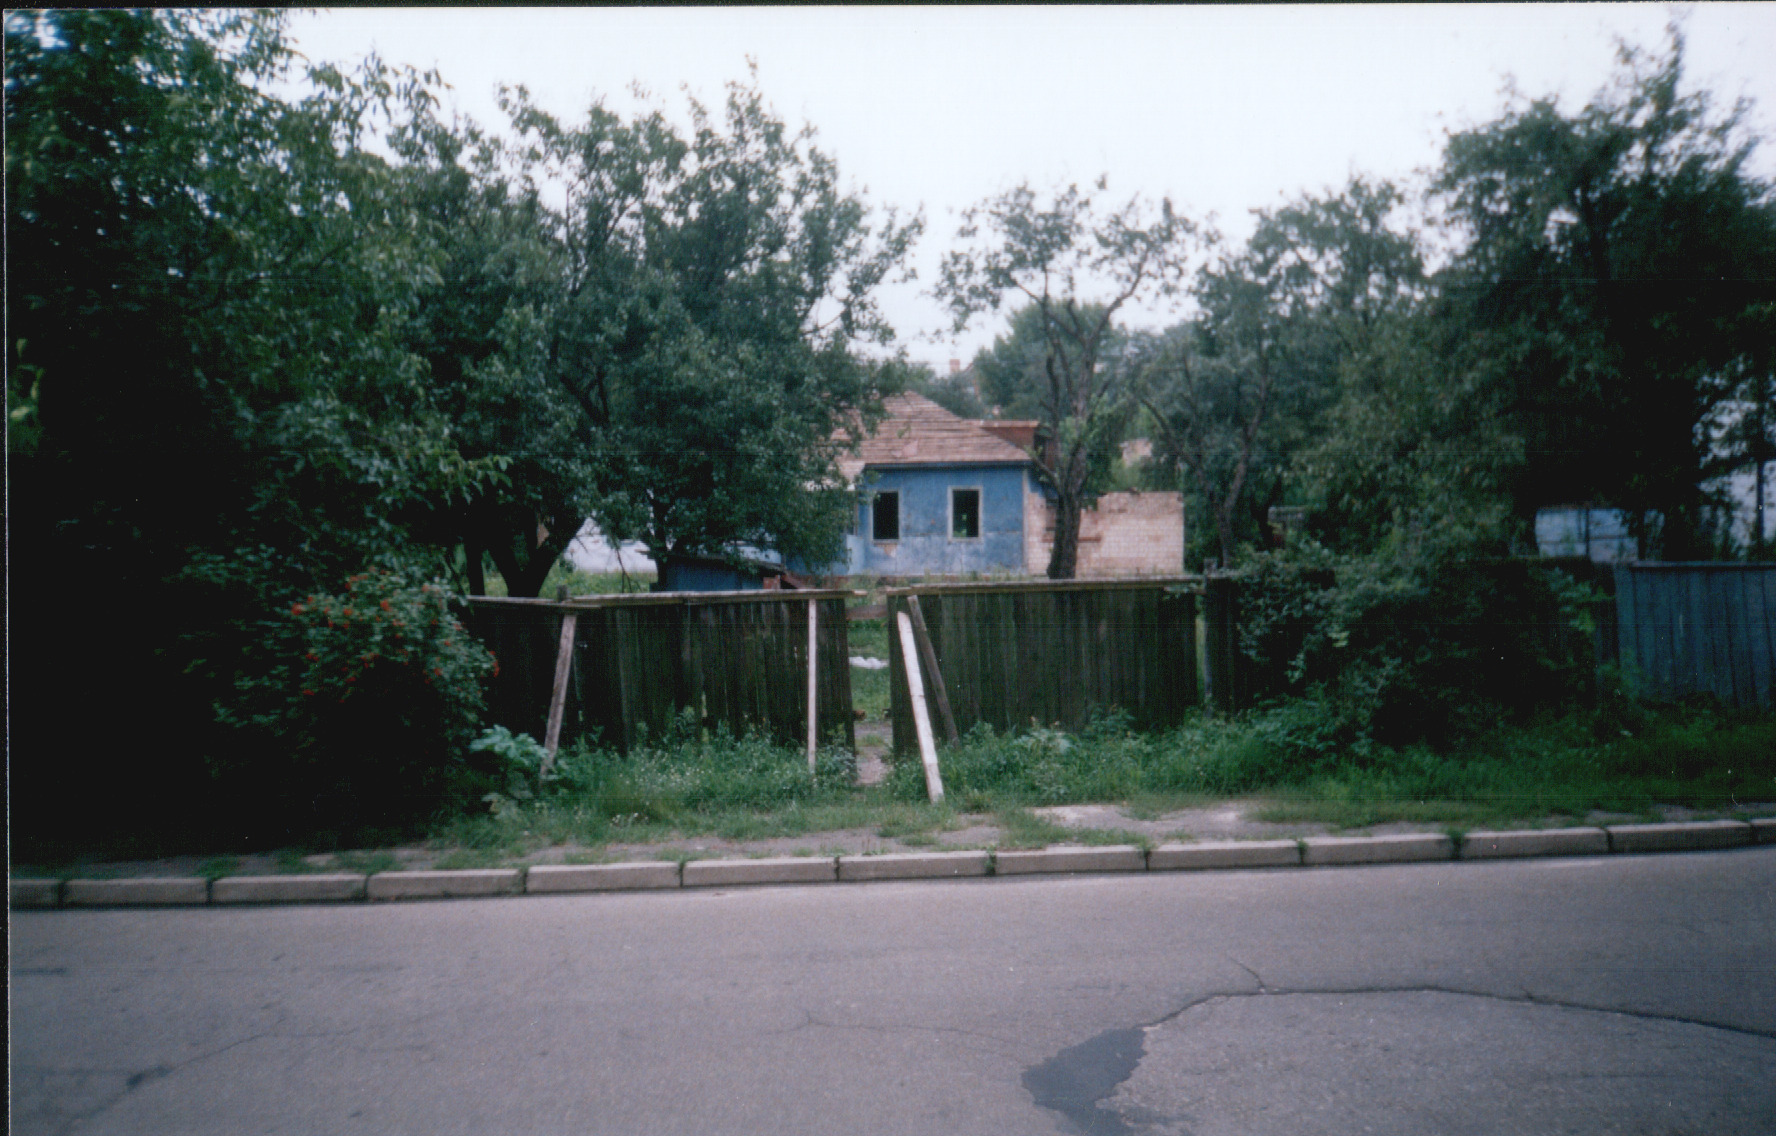
\includegraphics[width=\linewidth]{chast-vosp/zver/out0015.jpg}

\textit{2003 год. Ближе к низу Тимирязевской.}
\end{center}


Вдоль проулков, огибая кривые почтовые ящики, синие и ржавые, темными влажными полосами стекала вода из колонок. И катились, катились, чтобы сбиваться внизу в кучи – орехи, яблоки, сливы, лежали там вперемежку с коричневой и сырой прошлогодней листвой, прели. То был запах осени. Знай, ибо ушел отсюда этот дух.

Часть района вдоль Тимирязевской начала искажаться еще в девяностые. Покинутые одна за другой усадьбы разваливались на глазах. Ранней весной 1993-го я зашел в полуразрушенный дом и вытащил из обломков «Пиковую даму» издания 1938 года, размокшую от снега настолько, что я не мог расцепить страницы. Дома просушил, но бумага стала рваться, пришлось выбросить.

%Это ее владельцы могли слышать, как ездил по окрестностям, в раздолбанном мотоцикле с коляской керосинщик и кричал: «Карасин! Кому карасин?». Покупали его для плит и ламп.

В детстве мы много гуляли по Тимирязевской до самого низа, к той дельте ручья под обрывом с ракушками, о которых я рассказывал в начале книге. Да и на санках катался от верха и почти до половины улицы, хоздвора. 

Помню, еду вечером, в тишине только полозья шипят. Фонари оранжевый свет бросают, под ним снег фиолетовый, да еще искрой поигрывает. Я каблуками притормаживаю, поворачиваю, и рядом Бобик бежит, за сапоги азартно схватить пытается.

Долгими следами укатана улица. Навстречу идут уже съехавшие дети, тянут за собой на веревочках санки. А много еще шагать.

\begin{center}
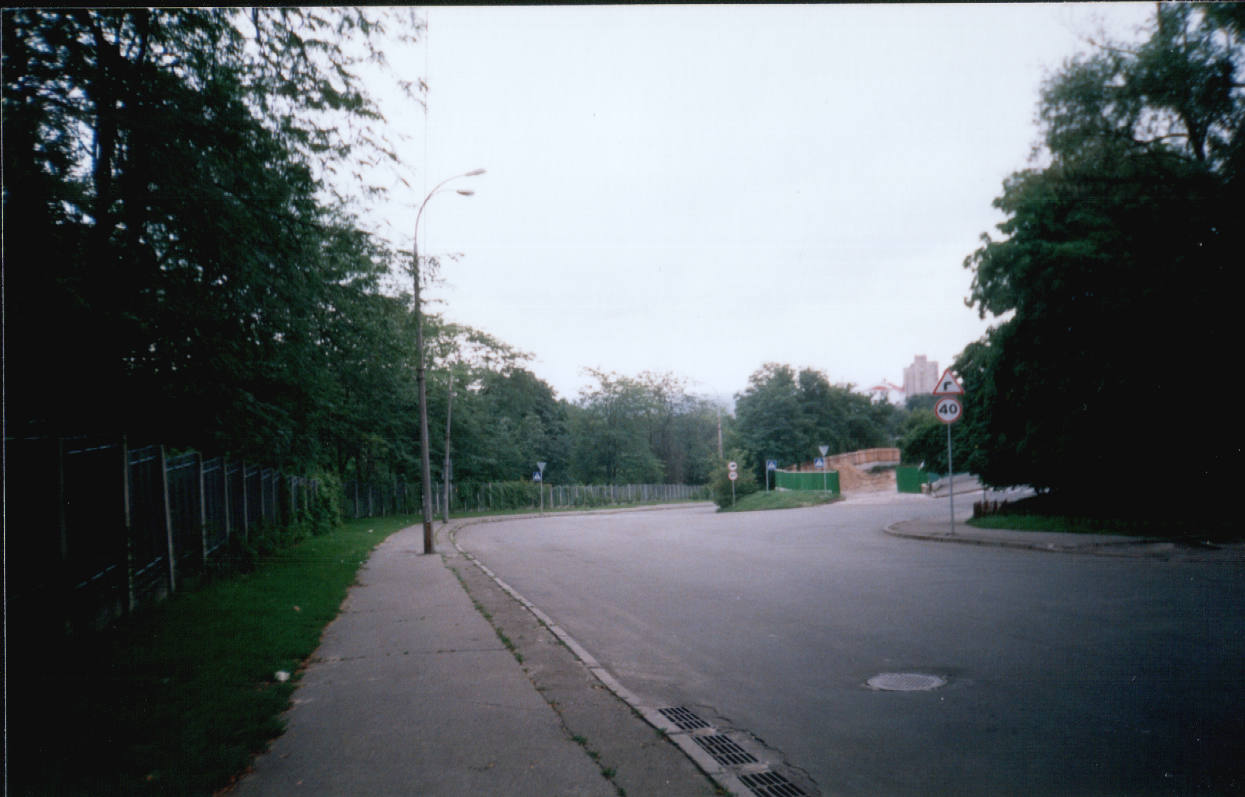
\includegraphics[width=\linewidth]{chast-vosp/zver/out0026.jpg}

\textit{2003 год. Верховье Тимирязевской.}
\end{center}

Эта часть Тимирязевской раньше называлась Омелютинской улицей, от местного жителя по фамилии Омелюта, обитавшего здесь по крайней мере в 1880х. Там когда спускаешься, за оградой ботсада тянется участок вьющихся растений. Восточнее него – Кленовая аллея, прежняя улица Еврейская (которой почти параллельно шла Ерейскокладбищенская, ныне аллея что начинается прямо от входа во Вьющиеся). На участке этом было кладбище евреев, основанное в 1798 году (а на плане 1879 года к нижней части иудейского примыкает «татарское кладбище»). Закрыли же его в 1895-м, но продолжали ухаживать. Сахарные магнаты Лев да Лазарь Бродские в 19 веке обнесли это кладбище стеной каменной да позже сами за нею упокоились. И где их прах? Смешавший его с землей варвар, во время Затонского неистовства в 1930-х, тоже давно умер.

Поныне можно найти остатки надгробий – на горке кактусовых, и вообще в околицах вьющихся, особенно в сторону хоздвора. 
Также каменные надгробия использованы в опорной стене у института Проблем прочности, от его входа и к дому номер 4 по Тимирязевской.

А мы там гуляли. Тимирязевская поворачивала. Справа продолжался частный сектор, слева сквозь прутья забора, поросшего хмелем и диким виноградом, виднелись в барвинковом ковре под пригорком корявые деревья. Затем – частная усадьба и магазин от ботсада. Внутри пахло горшками с землей и цветами.

\begin{center}
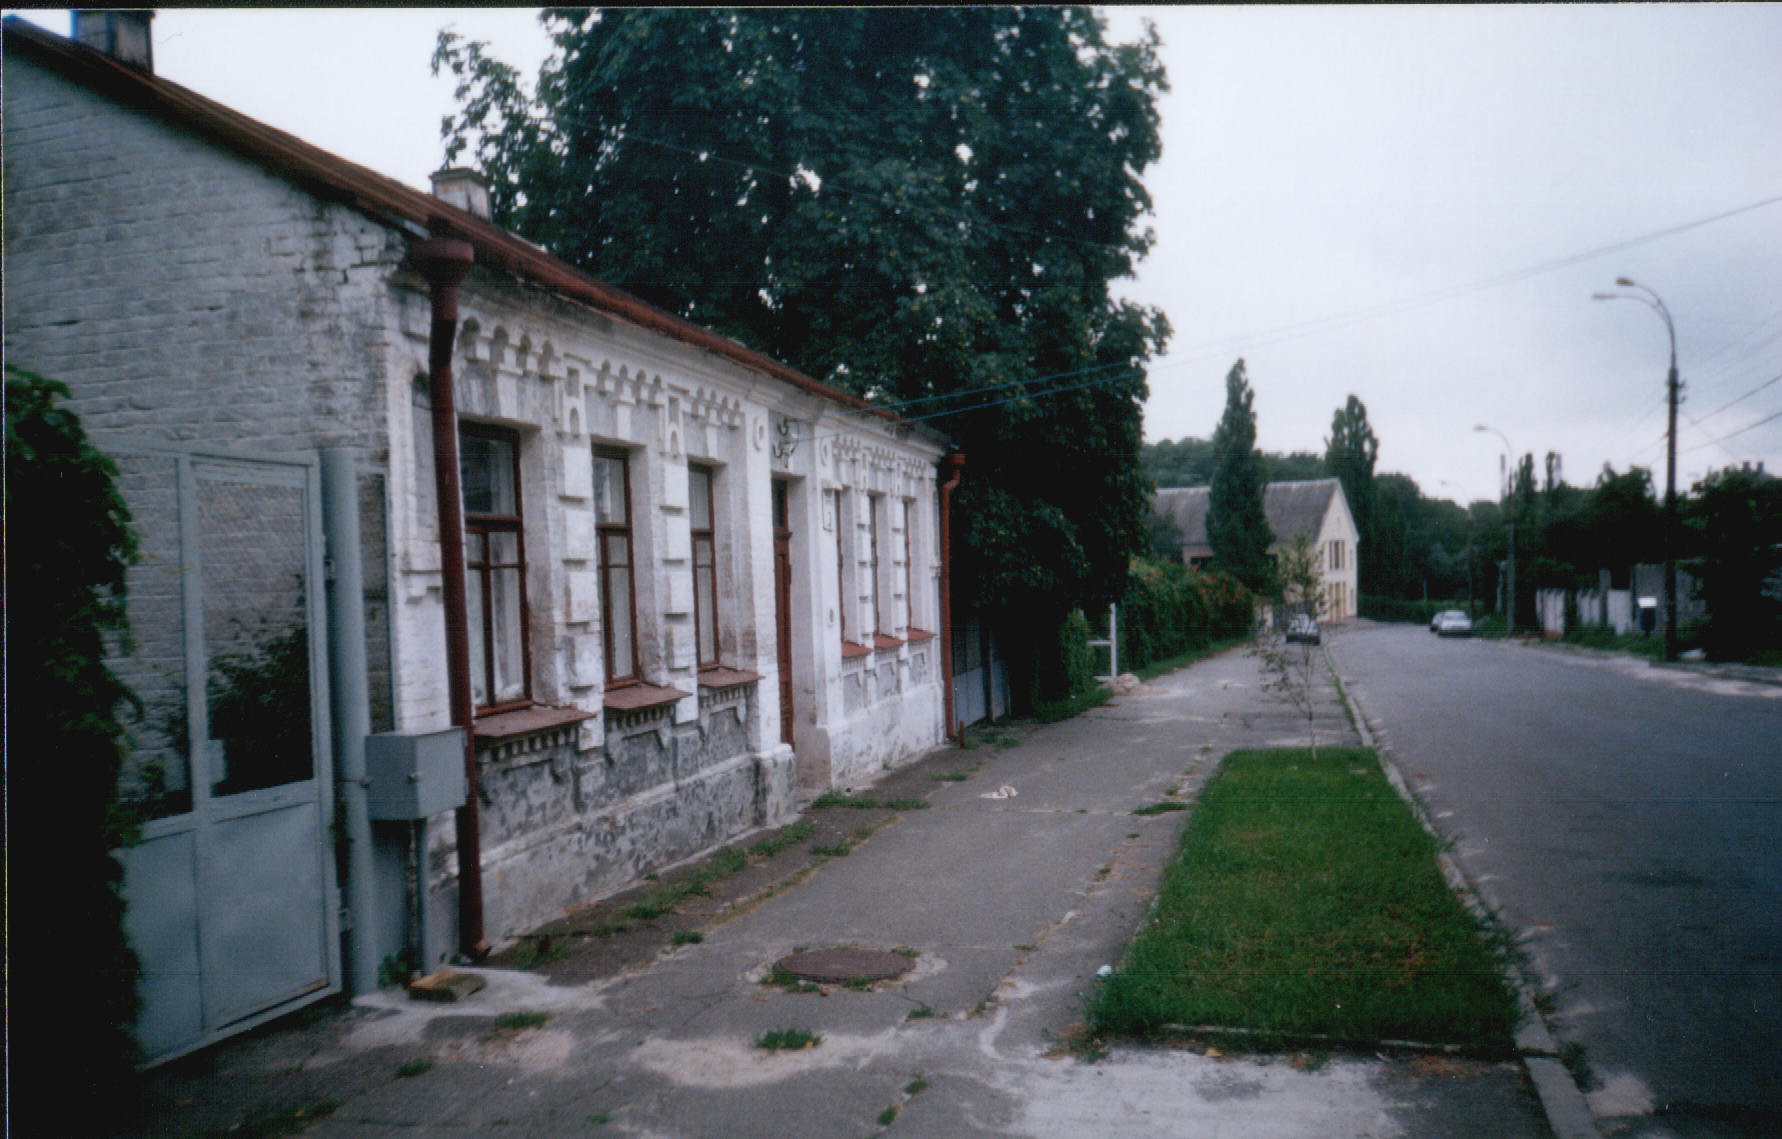
\includegraphics[width=\linewidth]{chast-vosp/zver/out0014.jpg}

\textit{2003 год. Середина Тимирязевской.}
\end{center}

Затем мы доходили к старому, похожему на дом культуры сталинских времен, зданию ботсадовского хоздвора. За ним есть несколько подобных строений, в том числе жилое, да разные гаражи и мастерские с тракторами, сеялками, веялками.

Вторая, нижняя половина Тимирязевской (примерно от пятой школы) – была отдельной улицей, Военно-кладбищенской, называясь от близости к Госпитальному, или Военному кладбищу, что в самом низу, над Теличкой.

Про ручей Омелютинку, выходящий на поверхность около хоздвора, сведений очень мало. Название известно по молве работников ботсада и связано то ли с жителем Омелютой, то ли Омелютинской улицей. Левый берег ручья представляет собой высоченный суглиновый склон, именуемый старожилами горой Караваевкой, от местности Караваевщины, про которую я расскажу чуть позже. 

По другую сторону ручья, вне ограды ботсада – Тимирязевская улица, там склон более пологий, то уже Бусова гора. Но между забором и склоном Караваевки есть всё же отдельная ложбина, то есть дно оврага ниже уровня улицы, и представляется, что прежде воды там было больше, а не как сейчас – среди бурелома и травяных кочек журчит, перекатываясь кое-где на небольших порожках, тонкий ручеек с песчаным плоским руслом, что временами приближается к пригорку с забором, а местами растекается в несколько рукавов, там, где самая низина расширяется, заставляя думать о том, что прежде здесь были пруды или болотца.

Заросли вокруг ручья кишат клещами. Водичка с виду чистая, на вкус не пробовал. Ручей выходит на поверхность в овраг, из бугра\footnote{50°24'31.5"N 30°33'32.7"E} в ботсаду, напротив Зверинецкого переулка, что следует за переулком Гастелло.

Всё поверхностное течение до ухода в коллектор и окрестности показаны нами в фильме «Киевская сюита». Причем ближе к порталу коллектора мы нашли, в труднодоступном месте, и сняли на видео, странные миниатюрные береговые укрепления.

Вдоль ботанического берега Омелютинки над ручьем идет добротная тропа, куда можно свернуть с липовой аллеи\footnote{Многие не знают, что кроме Липовой аллеи около «зимнего» входа в ботсад, есть еще одна, вот здесь – 50°24'35.5"N 30°33'33.7"E. На ней, кстати,вы увидите и любопытный суглинистый обрыв.}, если двигаться от хоздвора и потом сойти направо. Идя по тропе примерно ниже школы, в укромном месте, по левую руку, за буреломом есть засыпанный вход в подземелье, кирпичная арка (в своде видна арматура) у подножия\footnote{~50°24'23.4"N 30°33'35.6"E}. Неподалеку, с той же стороны, лежат некие черные тёсаные камни.

Еще в начале 20 века, там где тропа, то бишь на уступе над левым берегом ручья, стояли частные дома, а через ручей были перекинуты несколько мостиков – а напротив вливания Зверинецкой в современную Тимирязевскую целых два, побольше и поменьше.

Омелютинка уходит в едва пролазную трубу около забора Зеленстроя, и нею течет в Выдубицкое озеро, но я уже писал об этом подробно в первой главе.

Диггеры именуют Омелютинку Зверинецким ручьем или Net cave (из-за паутины в коллекторной его, нижней части) и утверждают, что исток его находится ближе к верху ботсада, возле Института проблем прочности. Но истоков было несколько.

Один исток прослеживается вдоль аллеи от Зимнего сада вниз к Японскому саду. Другой исток несколько восточнее\footnote{50°24'47.3"N 30°33'47.5"E}. На кем был, как минимум с 19 века, пруд. Японский сад лежит за земляной плотиной тоже в бывшем пруду. Следом – снова плотина, и общее русло ручья (на поверхности не виден) продолжается до хоздвора по оврагу у подножия большого холма участков «Лес украинской равнины», «Алтай и Сибирь», «Кавказ».

%Сохранились сведения о мостке через ручей между Караваевыми дачами и еврейским кладбищем.

Местность на холме с середины 19 века называлась Караваевщиной, или Караваевой дачей. Дача называлась «Прибрежной отрадой» и принадлежала хирургу и окулисту, профессору Владимиру Караваеву, что владел одноименными Караваевыми дачами за Шулявкой. Затем дачу выкупил Горащенко и превратил в хутор. А уже на стыке 19 и 20 веков там были  мелкие частные усадьбы. Утыканная домиками с огородами Караваевщина включала в себя и участки ботсада, где теперь плодовые сады, и степи Украины с современными  курганами, на коих стоят каменные бабы.

Аллея от перекрестка под Ионинским монастырем наверх была ненаселенным началом Печерско-Караваевской улицы, что лежала от верха Степей Украины и потом вниз между садами\footnote{От 50°24'50.19"N 30°33'48.96"E, через 50°24'41.8"N 30°33'53.41"E, до 50°24'21.66"N 30°33'45.84"E.}. 

Итак, начало бывшей улицы – перекресток около скамьи под навесом. Оттуда же на запад и потом параллельно улице отходил Печерско-Караваевский переулок. Следы его приметны поныне, он лежит по периметру хозяйственной территории с парой низеньких домиков.

В 1940 году улицу переименовали в Грибоедовскую, а до 1945-го она перестала быть улицей в связи с сооружением ботсада и сносом жилых домиков, хотя некоторые усадьбы были сохранены под жилье сотрудников ботсада. Из списков улиц удалена только в 1977-м. В первом десятилетии 20 века на ней было около тридцати усадеб, и примыкал Печерско-Караваевской проулок о десяти домах.

\begin{center}
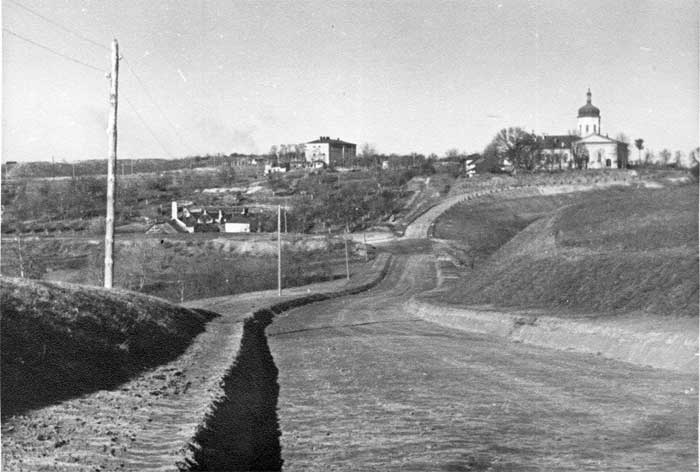
\includegraphics[width=\linewidth]{chast-vosp/zver/karavaevskaya.jpg}

\textit{Начало 1940-х. Вид на Ионинскую церковь. Застройка Караваевской улицы будет за спиной фотографа.}
\end{center}

На снимке – уже строится ботсад. Камера обращена к северо-западу. 

От нас вниз уходит дорога – на некоторых картах она считалась Караваевской улицей, а на деле лишь соедияняла перекресток с населенной слободой Караваевщины.

Впереди, слиянье трех дорог – развилка с добравшейся сюда улицей Еврейскокладбищенской, она присоединяется слева. Само кладбище было много левее. Многоэтажное здание в середине стоит и поныне в ботсаду, около перекрестка у верха Сиреневой аллеи, имеет адрес Тимирязевская, 47.

На холме справа – Ионинская Святотроицкая церковь, перед нею заметен, кругло расставивший ветки, древний дуб, он заслоняет левую часть храма. В ботсаду это не единственный многовековой дуб. Другой растет под аллей, ведущей по краю участка хвойных, над сиреневым садом. Мало кто знает, что сия аллея – прежняя улица Землянская.

Кстати учитывая древнюю дубраву на соседней Лысой горе, предположу, что дубрава покрывала некогда и Зверинецкий холм. Не от слова «дубы» ли Выдубы? Хотя предание о «выдыбании» здесь идола наверное более обосновано, чем моё предположение.

Сейчас всё выглядит примерно так же. Холмы никуда не делись, только ближайший справа стал много выше. А под дорогой, опоясывающей гору с Ионинской церковью, находится сад магнолий. Всё в них крупно – и листья, и розовые да белые, с кулак, цветы. Прямо на торт просятся.

До революции, среди монастырей Киева, Ионинский уступал посещаемостью лишь Лавре. Поначалу в нем было два храма. Покровский стоял на месте, где, по утверждениям монаха Ионы (Иоанна Павловича Мирошниченко, 1802-1902), ему явилась Богородица. Покровский храм разрушили в тридцатые годы. Он находился, насколько я знаю, двумя террасами ниже, в саду с райскими яблочками, откуда к Выдубичам пробивается через крапиву старинная кирпичная лестничка.

Уцелел Свято-Троицкий собор. Именно его видно на горке. Построен в 1871-1872 годах по проекту военного инженера И. Антонова, тогда же расписан художником Дмитрием Зайцевым, «открывшим» Зверинецкие пещеры. В 1897-м храм расширили – как начертал архитектор Владимир Николаев.

По его же проекту собирались возвести поблизости и 110-метровую колокольню выше Лаврской. Тогдашний митрополит Флавиан дал согласие построить сначала несколько ярусов с временной крышей, повесить колокола, затем изыскать средства на постройку рядом храма, размером соответствующего грядущей великанше, и уже тогда достраивать колокольню. Впрочем, смерть Ионы, Русско-японская война и путаница с финансовым положением монастыря остановили дело.

Новый настоятель, Мельхиседек, привлек внимание начальства своим обращением с денежными средствами. В обитель направили ревизионную комиссию, руководитель коей сообщал Флавиану:

\begin{quotation}
Усиленные занятия по обследованию хозяйственной части Киево-Троицкого монастыря вредно отразились на нервной моей системе, я стал страдать бессонницей, и, кроме того, явились головокружения, чего прежде у меня не было, а потому смиреннейше прошу Ваше Высокопреосвященство освободить меня от производства сего следственного дела.
\end{quotation}

Мельхиседека могли привлечь даже к уголовной ответственности, но взамен отстранили от управления монастырем и направили в Соловки, а путаницу  денежного учета Консистория пояснила обыкновенным невежеством:

\begin{quotation}
Если принять во внимание, что архимандрит Мельхиседек обучался лишь в двуклассном министерском училище и не изучал ни бухгалтерии, ни счетоводства, то многие неправильности в ведении им сложного и большого хозяйства Свято-Троицкого монастыря с многотысячными оборотами можно объяснить его невежеством, неподготовленностью и незнакомством с техникою ведения отчетности в столь сложном деле.
\end{quotation}

Готовые полтора яруса колокольни – черная дыра, куда ушли деньги – были разобраны в 1920-х на кирпичи для постройки Киевской сельхозакадемии в Голосеево.

%Вот снимок, сделанный несколькими десятилетиями раньше предыдущего:

\vspace*{\fill}

\begin{center}
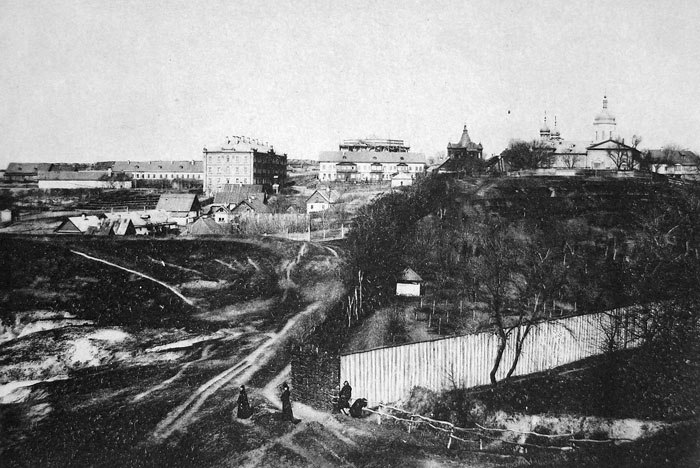
\includegraphics[width=\linewidth]{chast-vosp/zver/karavay.jpg}

\textit{Рубеж 19 и 20 веков.}
\end{center}

\vspace*{\fill}


Эта фотография снята, как если стоять спиной к теперешнему участку «Карпаты». Распутье дорог.

Вот от середины строго налево пошла грунтовая дорога к Печерско-Кара\-ваевской улице. А домов сколько спереди  слева – по Еврейско-кладбищенской!

Справа внизу, где на фотографии отдыхают люди – сейчас начинается участок Карпаты. Примерно там же, по ложбине, на восток к набережной вела широкая тропа. Следы ее прослеживаются поныне.

Что за строения примыкают к Ионинскому Святотроицкому монастырю? Четырехэтажный дом для монахов (а их было около полутысячи), гостиницы для паломников,  корпуса для паломников, школа, больница, мастерские.

\newpage


\begin{center}
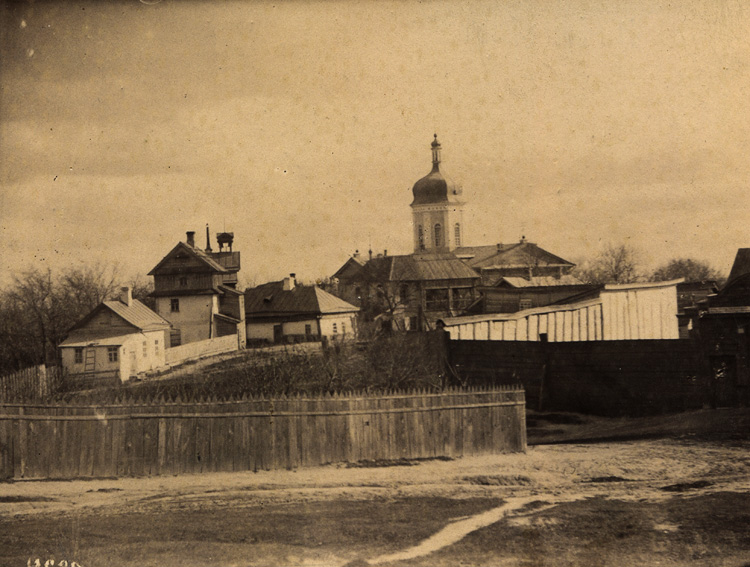
\includegraphics[width=\linewidth]{chast-vosp/zver/1890x-ion.jpeg}

\textit{1894 год. Вид на Ионинский монастырь со стороны верха Сиреневой аллеи.}
\end{center}
\vspace*{\fill}


\begin{center}
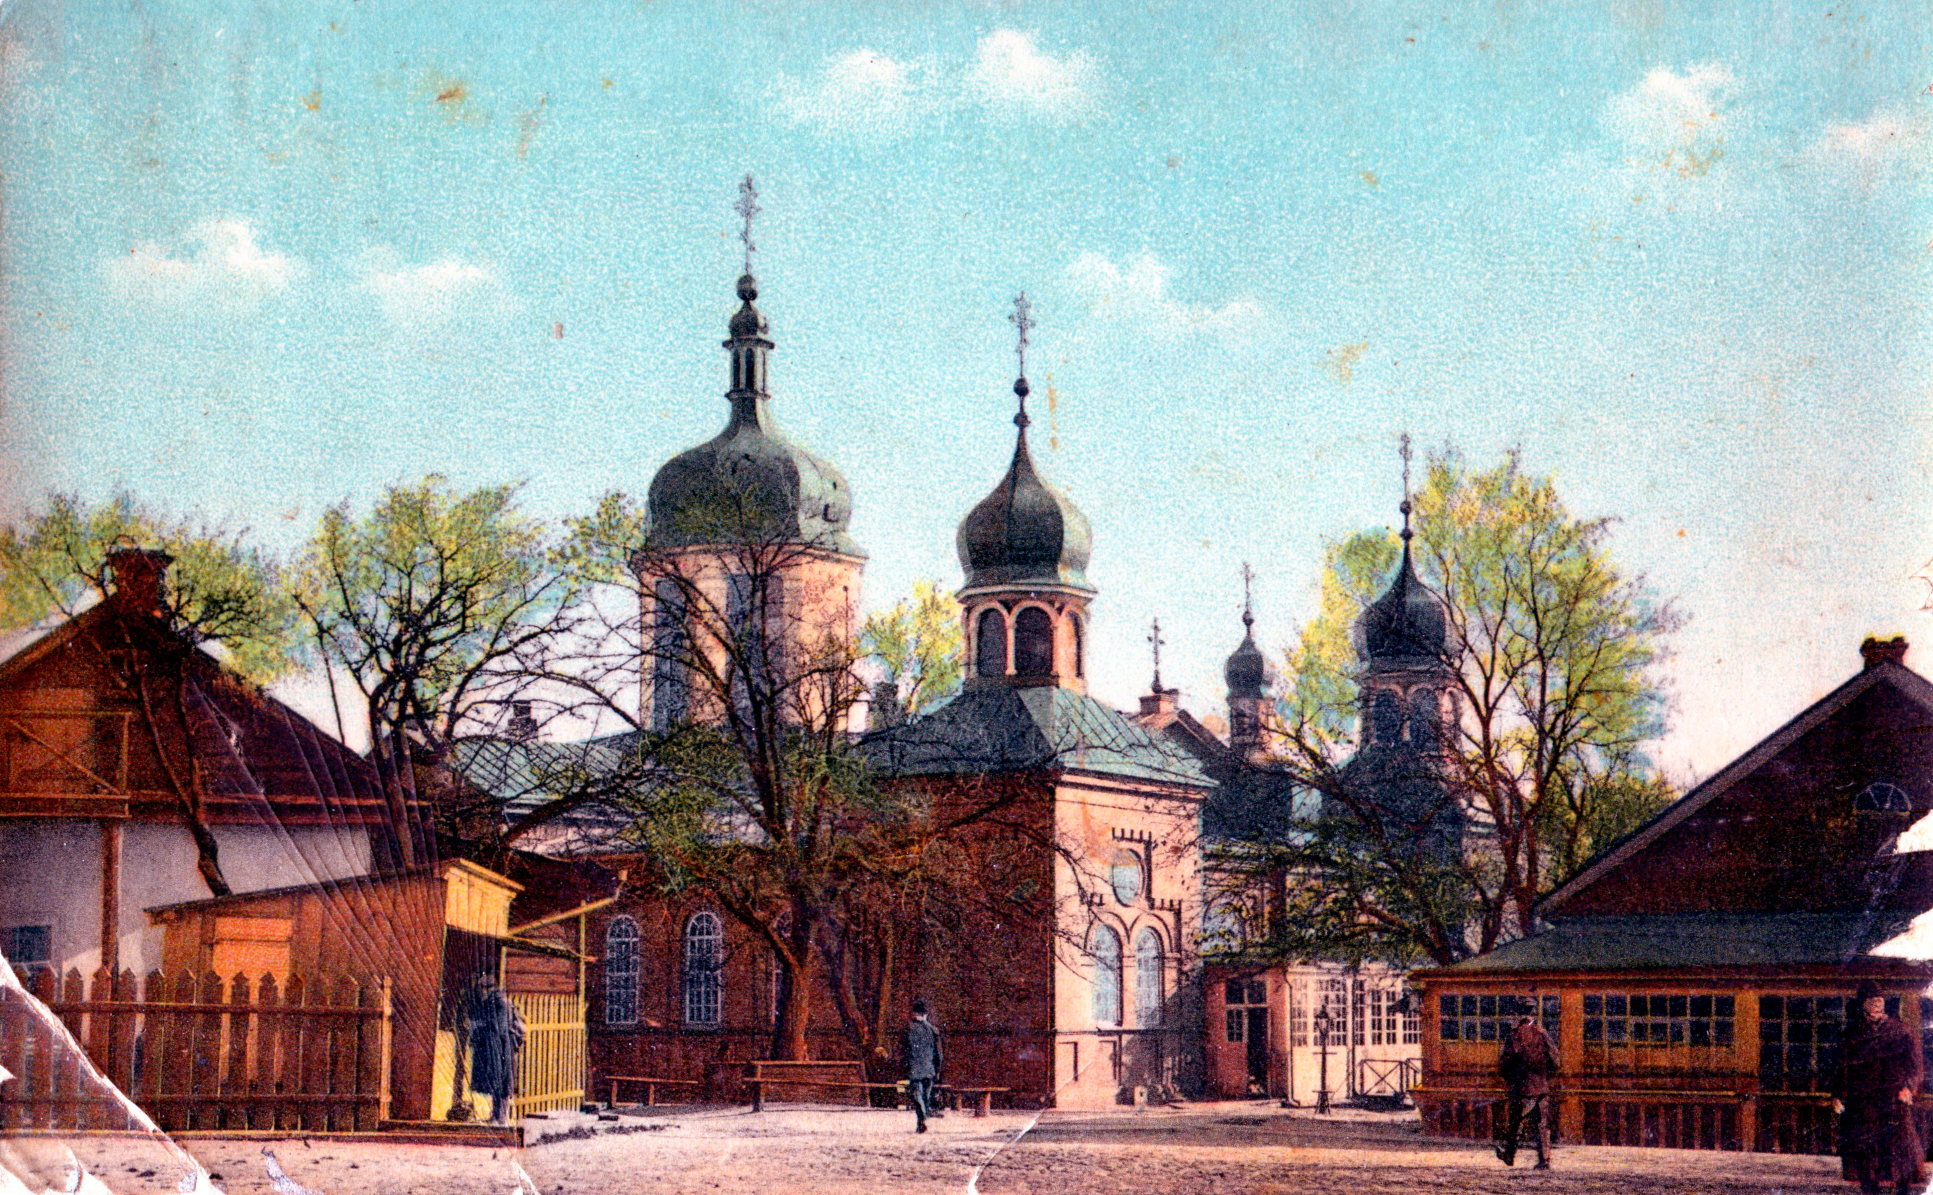
\includegraphics[width=\linewidth]{chast-vosp/zver/s-ion-complex-02.jpg}

\textit{На территории монастыря. Стык 19-20 веков.}
\end{center}
\vspace*{\fill}


\newpage
\vspace*{\fill}
\begin{center}
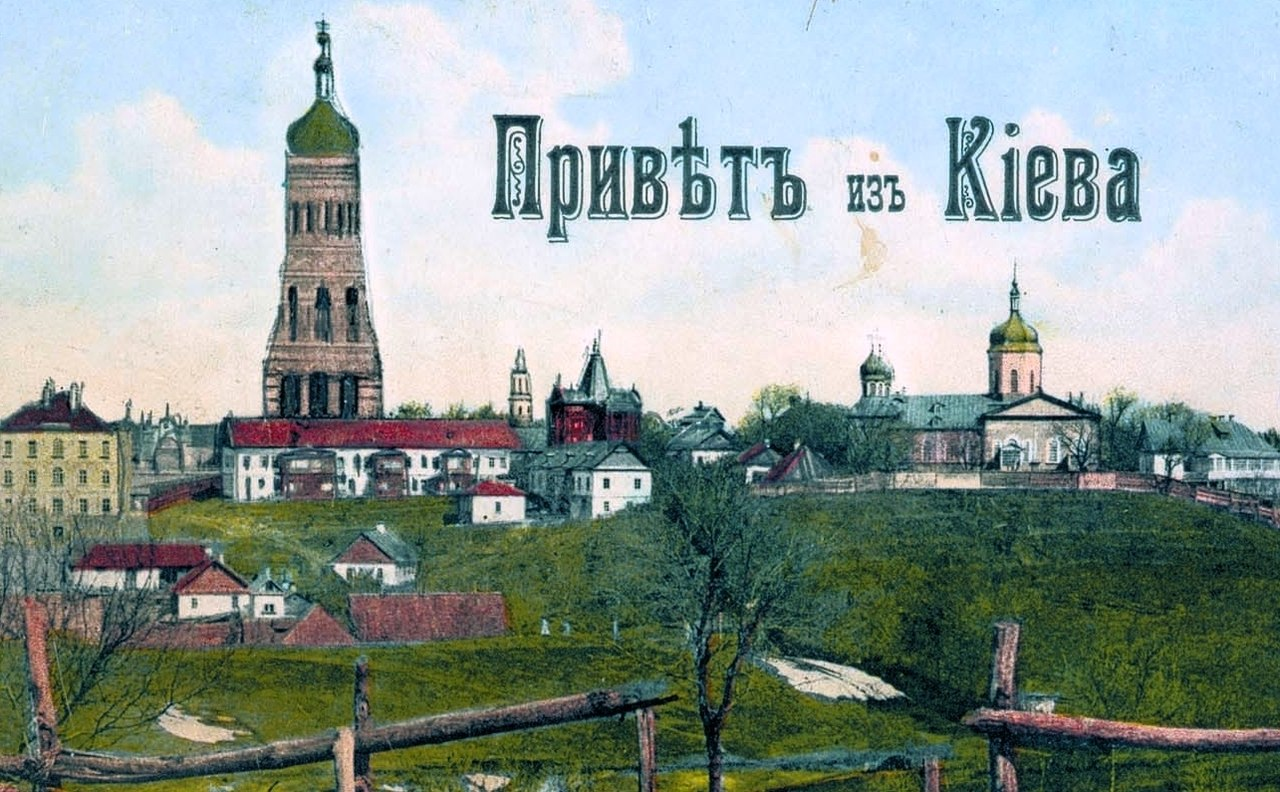
\includegraphics[width=\linewidth]{chast-vosp/zver/kolo01.jpg}

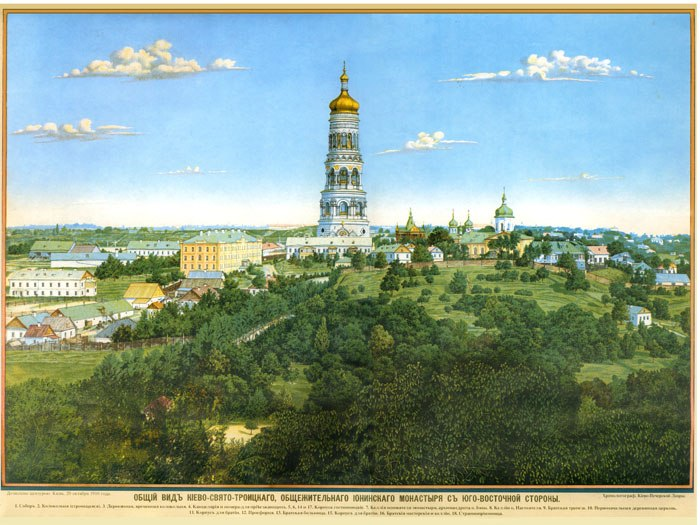
\includegraphics[width=\linewidth]{chast-vosp/zver/kolo02.jpg}

\textit{Старинные открытки опережают события, изображая  колокольню-великаншу. Ракурс выбран так, чтобы по возможности скрыть на горизонте Лавру.}
\end{center}
\vspace*{\fill}
\newpage

\begin{center}
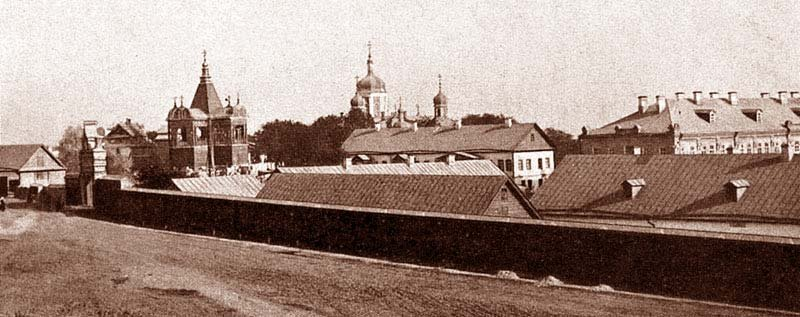
\includegraphics[width=\linewidth]{chast-vosp/zver/ion-complex.jpg}

\textit{Дореволюционный снимок Ионинского монастыря.}
\end{center}

Какие старые монастырские постройки уцелели поныне?

Старенькая двухэтажная часовня, что стоит над склоном, позади новой копии 2001 года, была построена в 1887 году. Там располагалась церковная лавка и башенные часы, изготовленные в 1858 году в Париже. Одного завода часов хватало на 6-7 дней. Они не прекращали отбивать на всю округу каждый час ни до революции, ни в советское время, ни сейчас. Уже во втором десятилетии 20 века магазин переделали под жильё. После возведения копии здания, часы перенесли туда.

Трехэтажный братский корпус с больницей, на уступе горы ниже часовни. На 2020 год пребывал в запустении, с выбитыми окнами. В восьмидесятых это был корпус, где работали сотрудники ботсада и находилась столовая. Мы с мамой, гуляя заходили туда и покупали пирожные – язычки и слойки. Рядом, под холмом, в железных клетках стояли сельскохозяйственные машины. 

Помню мотокосилку и грузовой, трехколесный мотороллер «Муравей» с кузовом и возможностью крепления спереди насадки для опять же скашивания травы. Монашеский корпус построили в несколько этапов, в 1912-1916 годах по проекту архитектора М. Гарденина с поправками епархиального архитектора Е. Ермакова. В здании работали иконописная и швейная мастерские. Хотя в монастырских бумагах указано, что здесь была больница, на деле оная обреталась около церкви в одноэтажном деревянном домике 1865 года, снесенного в 1940-х.

Розовый одноэтажный домик начала 20 века. Если спускаться по Сиреневой аллее, будет слева. Это прежние мастерские – слесарная, столярная, кровельная. С дореволюционных времен осталось также четыре погреба.

Так вот про ручей Омелютинку. В месте бугра за хоздвором ботсада, откуда она теперь вытекает, по 1940-е годы была гать с трубой, а поверх оной переезд на Тимирязевскую, точно напротив Тимирязевского переулка. В ботсаду, по другую сторону дамбы, на юго-восток теперь аллея – прежняя дорога с Караваевщины. У ближайшего перекрестка\footnote{50°24'29.2"N 30°33'39.11"E} эта дорога сворачивала резко на север – теперь там широкая тропа.

Подобные дамбы через ручей поныне сохраняются выше по былому его руслу, в районе Японского сада. По крайней мере в середине 19 века, на его месте был заболоченный пруд, откуда и сочился дальше, на юг, в сторону хоздвора, ручей.

Постройки хоздвора – уголок сталинской архитектуры, а также теплицы и различные хозяйственные сооружения. Там же второй, служебный вход в ботанический сад, и ворота для заезда автомобилей. А вдоль всё продолжается Тимирязевская, но дома уже совсем другие, чем в памяти моей.

В девяностых, летом мы с братом ездили по окрестностям на велике. Саша на багажнике, я в седле. Особый кайф был добраться на Бусову гору до зловещих остатков Госпитального кладбища в конце Зверинецкого переулка, на пригорке у железной дороги. Сейчас там новостройки и какая-то стена, да крест соорудили, а было заросшее коноплей кладбище со старинными могилами. Мы слезали с велика, чтобы передохнуть, и представляли, что сейчас полезут живые мертвецы. Но у нас был надежный тыл – велосипед. Напугав себя разговорами о покойниках, мы с братом садились на велик и уматывали под горку – я привставал в седле, чтобы бороться с возрастающим наклоном переулка...

На одном из крестов кладбища виднелась надпись: «МАНЯ 1824», хотя по источникам, землю под кладбище выделили в 1878-м. Может, тут хоронили и прежде?

Госпитальное занимало весь южный склон Бусовой горы, от железной дороги по нынешнюю улицу Николая Соловцова включительно, покрыв глинища кирпичных заводов Киевского приказа общественного призрения, стоявшими вдоль подножия горы примерно до конца 1860-х. Низовье Зверинецкой улицы от поворота (у коего по 2015 год оставались деревянные домики) и улица Сорочинская проложены точно поперек кладбища. Остался только юго-восточный его уголок.

Оттуда открывался вид на тяжелую промзону Теличку и за нею – Лысую гору. Среди предприятий Телички наиболее известны ТЭЦ-5 и Дерево-обрабатывающий комбинат, построенный в конце 1930-х с попутным расселением рабочих в раскуроченном Ионинском монастыре. Частично обжита лишь улица Промышленная, откуда детей автобусом возили в школу №5 и 133-ю. 

Теличка подразделяется на Верхнюю и Нижнюю. Верхняя – низ Караваевщины, ботсада. А Нижняя Теличка – вне ботсада, за железной дорогой. В конце 19 века вся местность обозначалась на картах как «деревня Теличко». Со временем память о разделении Теличек стёрлась, и теперь Теличкой называют лишь плоскую промзону к юго-востоку от кладбища. 

В документе «Описанию Посполитым слободи Зверинця в Уезде киевском состоящого, учиненногое 1786 года», среди описаний владений да имуществ Выдубицкого монастыря сказано:

\begin{quotation}
Там же на Либеди между кирпичными артилерийскими заводами близ мельнички\footnote{Выдубицкая мельница, стояла на малой плотине на Лыбеди.} в обивательской избе Григория Телички продается только ценная горелка в оного обывателя монастирской посуды: кварта – 1; полкварта – 1; чвертка – 1, жестяныя.\end{quotation}

Так вот кем был Теличко или Теличка – обывателем, продававшим водку в своей избе! Вероятно, позже он разбогател на этом, раз на картах появилась «деревня Теличко».

\newpage
\vspace*{\fill}
\begin{center}
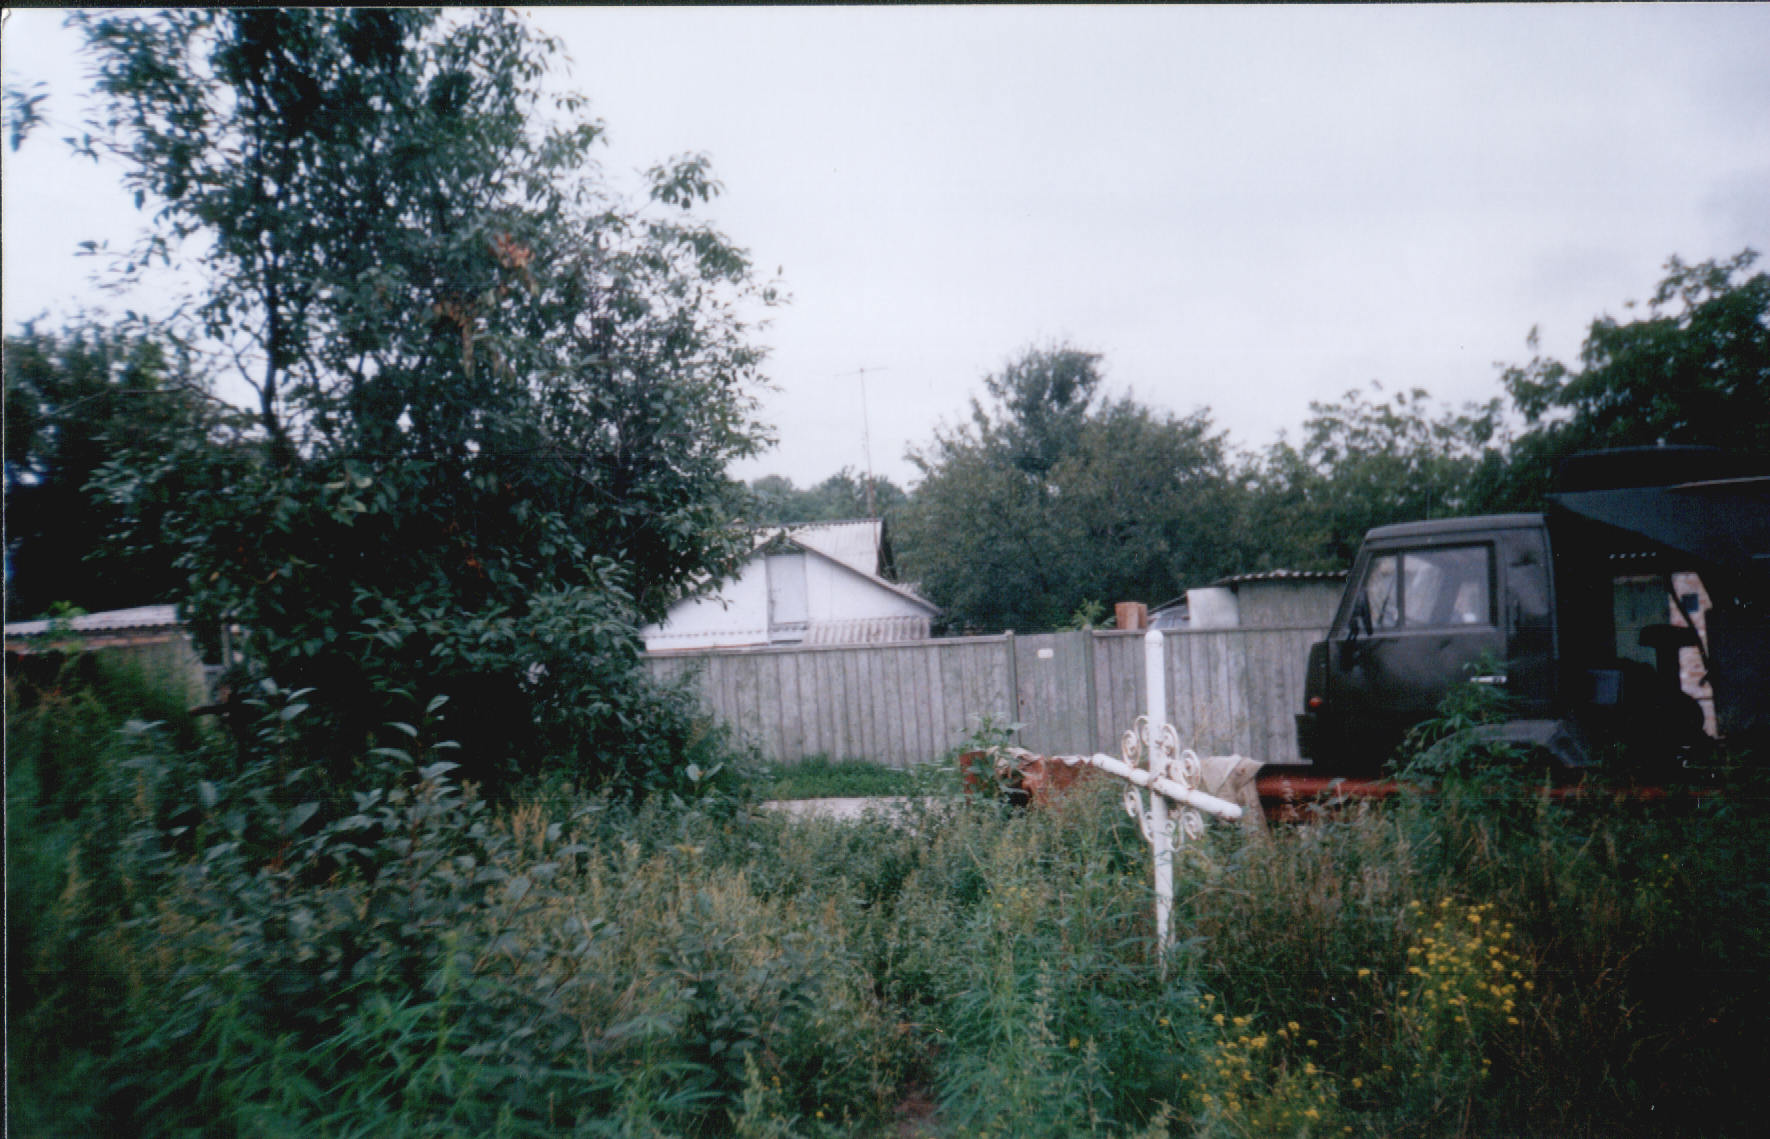
\includegraphics[width=\linewidth]{chast-vosp/zver/out0023.jpg}
\end{center}

\begin{center}
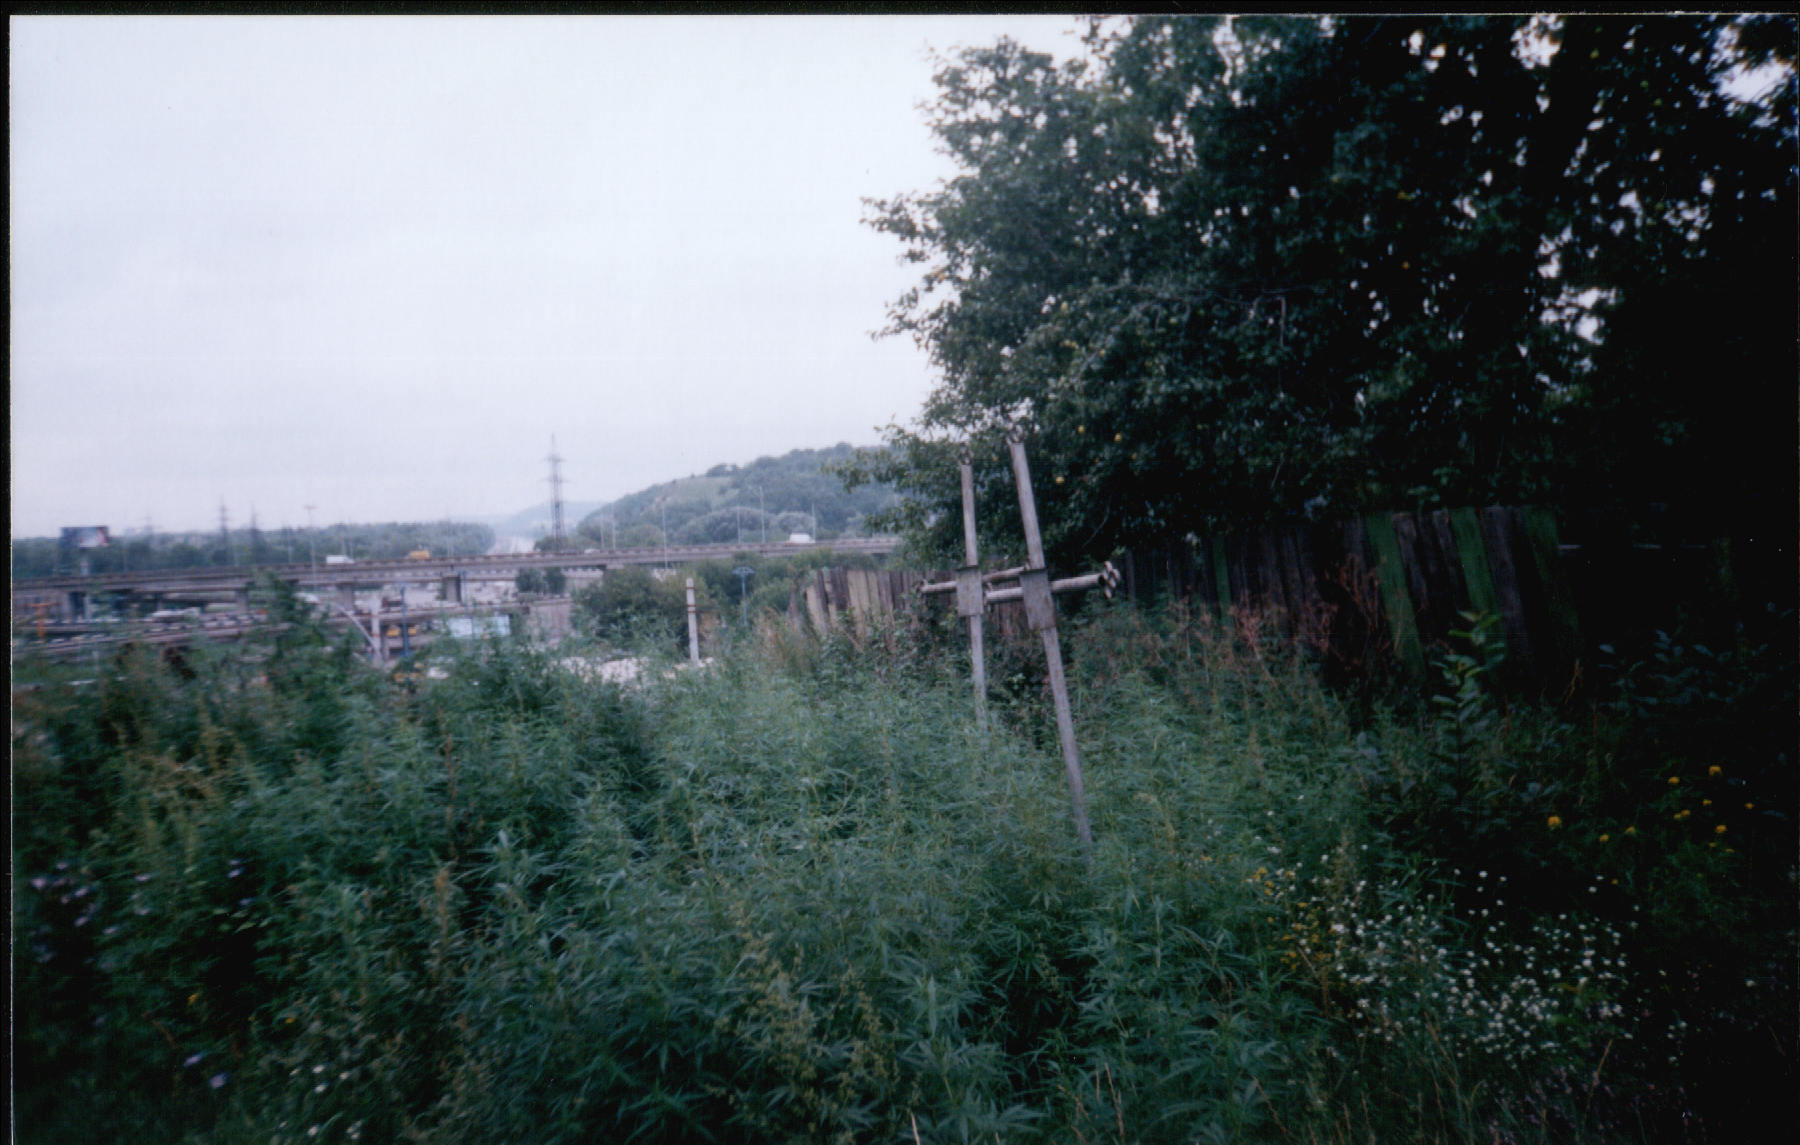
\includegraphics[width=\linewidth]{chast-vosp/zver/out0024.jpg}
\end{center}

\textit{Остатки Госпитального кладбища в 2003 году.}
\vspace*{\fill}
\newpage

%Там существует, кстати, запасная, глухая станция метро «Теличка»\footnote{50°23′47.19″N (50.396441), 
%30°34′19.11″E (30.571974).}, она же «Стройиндустрия». Поезда проезжают ее без остановки, двигаясь от «Выдубичей» к Южному мосту.

Самый низ улицы Тимирязевской, справа начинается пригорок с остатками Госпитального кладбища, часть Бусовой горы:

\begin{center}
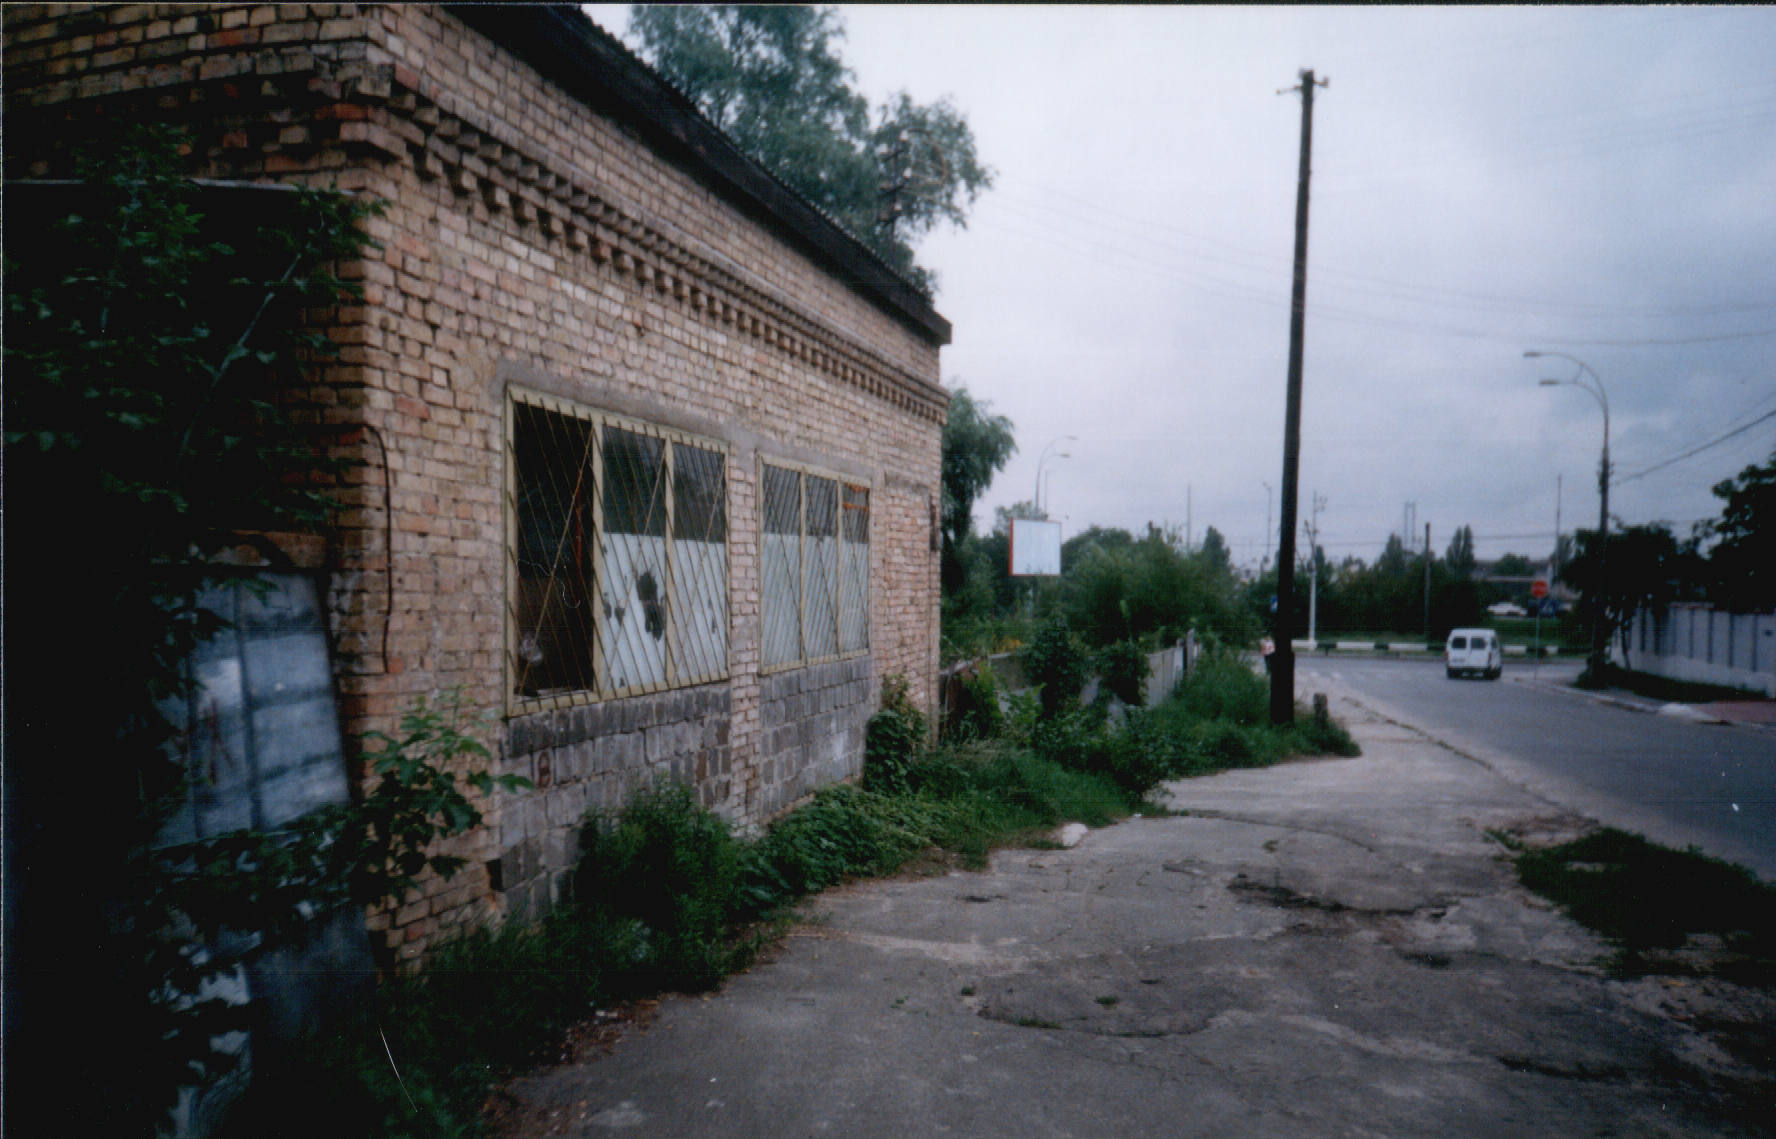
\includegraphics[width=\linewidth]{chast-vosp/zver/out0012.jpg}

\textit{Фото 2003 года. Слева бывшее здание магазина, сам магазин я в конце 80-х уже не застал.}
\end{center}

Слева, оттяпав часть дельты ручья, долгое время был какой-то склад, металлолома наверное. Во время создания снимка, ручей как раз загоняли в коллектор, над коим возвели потом здание Киевзеленстроя и теплицы. Часть былой растительности еще виднеется на фотографии – огромная ива.

Это сюда мы с мамой ходили к обрыву с ракушками (ибо мимо склона протекал некогда Днепр, да, так близко!), перебирались через ручьи между сырыми, покрытыми весенними цветами, островками земли. Отсюда смотрели на поезда – одна из причин прогулок «мимо ботаники».

Вернусь к Караваевщине. Когда я жил на Бастионной, то этого названия не слышал. Ботсад разбит на участки – Хвойные, Алтай, степь, сад магнолий, сиреневая аллея, прочее. Так и называли. Обитатели окрестных хрущовок не несли в своей памяти представлений о том, что находилось тут прежде.

На склоне горы над хоздвором мы брали лещину – там огромная роща лесного ореха. Тайком, пацанами, наведывались в плодовые сады – правда только несколько раз, ибо сады охранялись и можно было нарваться на сторожей, про которых ходили слухи, что те стреляют солью из ружей.

По рассказам я знал, что раньше, когда местные пытались воровать цветы из питомника рядом с розарием, сторожа таки палили солью, и «злодеи» подкладывали себе картонки сзади в штаны. Я уже не застал подобного рода приключений.

Однажды мы – я, Серый, Миша, Андрей, еще кто-то – отправились за алычой, желтой такой мелкой сливой. Осторожно пробрались, куда надо. А там два мужика алычу рвут, да в мешки! Мы пошли к сторожу и настучали ему на мужиков. Сторож прогнал их. Сад с алычой опустел, и к сбору урожая приступили мы.
 
Набили полные кульки, рюкзаки. Устало тащим назад, в открытую. Тут невиданное. Подъезжает к нам на «Волге» милиционер и недоумевает. А мы поясняем, что сторож – наш дядя, он разрешил! Милиционер говорит – несите всё к выходу, я буду там ждать. До сих пор ждет.

Но это были единичные вылазки, проще было собирать орехи и вишню на Собачке, яблоки в палисаднике за домом, а лещину рядом с березовой рощей и хвойными. У Собачки вдоль забора ботсада вообще лежали, почти бесхозные, огромные тыквы и кабачки. Рос топинамбур – земляная груша – вершки как у небольшого подсолнуха, но со съедобным корнеплодом.

Снова я отошел далеко. Караваевщина. На ее плоской верхушке есть участок Степи Украины, с несколькими курганами и большой горкой, что чертовым пальцем торчит в небо. Ее отовсюду видно. За ней скрыта еще одна, поменьше. Я любил перебегать с горки на горку.

Но больше всего мне нравились два низеньких кургана. На них стояли каменные бабы – настоящие древние идолы. Один куда-то умыкнули, потом взамен поставили другой, непонятный и красноватый. А из прежних уцелел лишь один, и у того в девяностые отбили голову да написали «ЦЕРКОВЬ СКАЛА». С этим курганом у меня связана затея детства – искать клад. Я же знал, что в курганах находят сокровища. И решил отправиться в экспедицию, раскопать курган. Я намеревался размочить его, твердый и суглинный, горячей водой, и потом уже рыть.

Начал готовиться. Завел коробку из-под обуви и написал поверх фломастером – «Кладоискатели». Туда стал собирать необходимое: кипятильник, несколько парафиновых свеч, веревку, металлический прямоугольный фонарик (питался от большой квадратной батарейки), перочинный ножик, спички, сухой спирт и прочую ерунду.  

\begin{center}
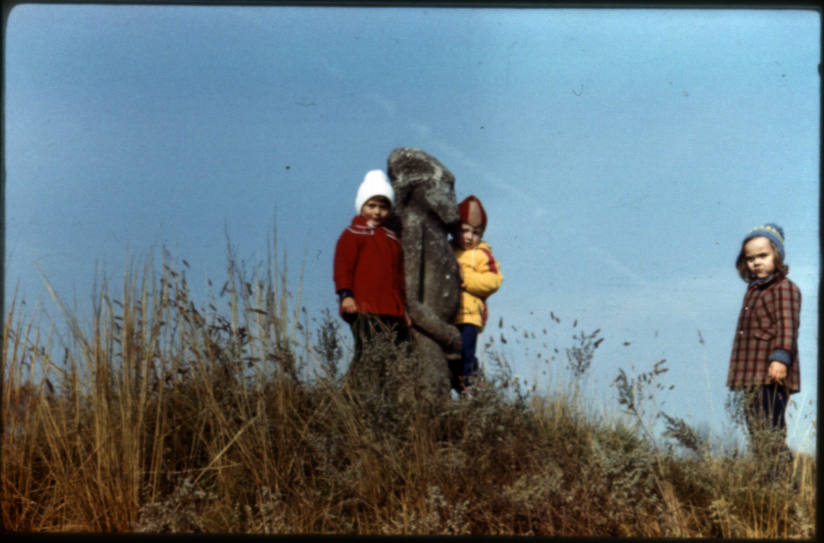
\includegraphics[width=\linewidth]{chast-vosp/zver/ya-na-kurgane.jpg}

\textit{Кажется 1980 год. Я – в желтой курточке.}
\end{center}

Пробовал подключить к экспедиции деда Шурика, но не вышло. А задумка рассосалась, я не мог придумать, как перетащить достаточно горячей воды. В термосе – мало, значит надо кипятить на месте, но кипятильнику нужно электричество. Отпадает! Я возлагал надежды на сухой спирт, для подогрева, однако требовался котелок. Было очень здорово вечером доставать эту коробку, перебирать вещи, и мечтать, что скоро экспедиция осуществится.

Близ Степей отвели под свалку обрыв. Мы с друзьями ходили туда искать батарейки от «Полароидов» – эта компания тогда выпускала фотоаппараты, которые сразу печатали и высовывали из себя готовый снимок, что желтел через пару лет. После печати оставалась черная пластиковая кассета-коробочка без бумаги, но с живой батарейкой. Приделываешь к ней маленькую лампочку, светишь. На той же свалке несколько месяцев подряд стояли довоенные швейные машинки «Зингер». Склон обрыва покрывала гнилая капуста, прочие овощи и строительный мусор. Сюда же свозились и кучами сбрасывались отходы из урн, расставленных по всему ботсаду.

При Советском Союзе и первые годы после, ботсад наполнялся только в дни цветения сирени. В остальное время можно было пройти всю боташу и почти никого не встретить. С 1990 года со мной по жизни шагал пёс Бобик, взятый на Куреневском Птичьем рынке. В девяностых собралась тусовка собачников из окрестных домов, в том числе Художников. Сначала мы все гуляли на Собачке, потом ходили в ботанический сад через дырку в заборе. Никто не видел, никто не гонял. 

У Бобика была подружка, эрдельша Даша, она рано умерла. Много кругов намотано с ней по ботсаду! Еще помню тоже эрдельшу Карму у художницы Солонько, что подарила мне картину с рябиной, вот она висит слева на стене. У нас в доме мало чужих картин. Несколько моих, несколько деда Павла, одна Солонько и одна – рисунок тушью с неведомым мне спаниэлем, приобретенный на самом первом киевском вернисаже на Андреевском спуске. Был еще спаниэль Бэк, но с Бобиком они стали драться и мы перестали с ним гулять. Ника – дратхаар, за которой Бобик далеко убежал и мы его искали. Белая, большая красивая дворняга Бим. Кто же еще? Овчар Найс, кавказец Каро. Где вы, добрые ребята?

Когда надоедал ботсад, я ходил с Бобиком в парк Примакова, или в Царское село и Наводничи, и по улице Панфиловцев, где стояли старые частные домики военных, да в ландшафтный парк под музеем Великой Отечественной Войны. Ботсад детства и юности оценен мною на вес золота позже, издалека. Возвращаюсь на Собачку, лезу в боташу через дырку. Я еще здешний!

Мы с Бобиком облазали почти всю Ботанику. И не ведали, что многие аллеи – былые улицы, а излюбленные места наших прогулок некогда покрывала Зверинецкая крепость.

5 июня (25 мая по старому стилю) 1918 года, в занятом немецкими войсками Киеве взорвались пороховые склады.

«На Лысой Горе произошел взрыв» – написал Булгаков в «Белой гвардии». И погрешил против действительности. Ведь рванул не Лысогорский, а Зверинецкий форт. Точнее, пороховые погреба в нем. Погреба – сказано громко. Деревянные сараи.

Зверинецкий форт построили в 1810 году на месте, где по крайней мере с середины 18 века жили «разных чинов люди», то бишь стояли небольшие домики с садиками. Неясно, какой была эта горная равнина прежде – может, холмистой, а при фортификационных работах ее сделали плоской. В других частях ботсада уцелели старые, многовековые деревья, здесь же вся растительность относительно новая, времен заложения ботанического сада. На картах форт выглядит белым пятном – таким же остается для нас прошлое этой части Зверинца.

%Что находилось на месте форта еще раньше? На карте 1745 года местность над Выдубичами, на восток (к саду сирени) и север через хвойные по нынешнюю улицу Мичурина занимали «строения разных чинов людей». Это примерно восточная половина будущего форта, с ощутимым довеском по краям в сторону Днепра и Неводничей. Одновременно это западная, от озера Святого, часть села Зверинец.

Крепость занимала большую площадь, которую с привлечением современных ориентиров опишу так – с севера границами форта был частный сектор по улицам Мичурина, Пырятинской и местности Землянке (Землянские улица да переулок). С востока – склон холма, где теперь «воссоздали» Красный двор (место спорное). С юга – аллея ботсада вдоль Горного сада, что перед розарием. С запада – липовая аллея до березовой рощи. В урочищах нынешнего ботсада, форт покрывал березовую рощу, хвойные, розарий и горный сад, включая обзорную горку над липовой аллей, около участка пряных и лекарственных растений. Эта горка была юго-западной частью Большого бастиона форта, впрочем высота ее много увеличена – я сам видел из окна, в восьмидесятых, как трудился бульдозер.

В склоне темнела большая нора или пещера. Я полагал, что в ней живет нечто страшное.

Под горой растет громадная ива. Мне нравилось, взобравшись по тропке на склон, подтянуть к себе ветвь – сноп желтоватых прутьев – и схватившись за них, высоко пролететь до ствола и потом обратно, на склон.

Время от времени кто-то ставил наверх, откуда весь ботсад виден, как на ладони, скамейку. Затем хулиганы сбрасывали ее в самый низ, то же проделывали с мусорными урнами. Гору, поросшую травой, нередко поджигали, и она горела вся, а ветер относил дым и пепел к нашим балконам.

Остатки форта сохранялись до окончания Великой Отечественной войны и были разобраны после нее, при постройке ботсада, пленными немцами. Разбирать пришлось много чего. Поныне остались земляные оборонные сооружения – валы, углами огибающие участки ботсада, что особо заметно в березовой роще и стороне розария, обращенной к горному саду. Всё это мы показали в серии «Киевской амплитуды» про Зверинецкий форт. 

На немецком аэрофотоснимке 1943 года, запечатлевшем форт с окрестностями, я подписал названия частей крепости и сделал цветные пометки. По сохранившимся ориентирам вам будет легко наложить картину на современность и всё сопоставить. Цветные линии – это улицы!

\begin{center}
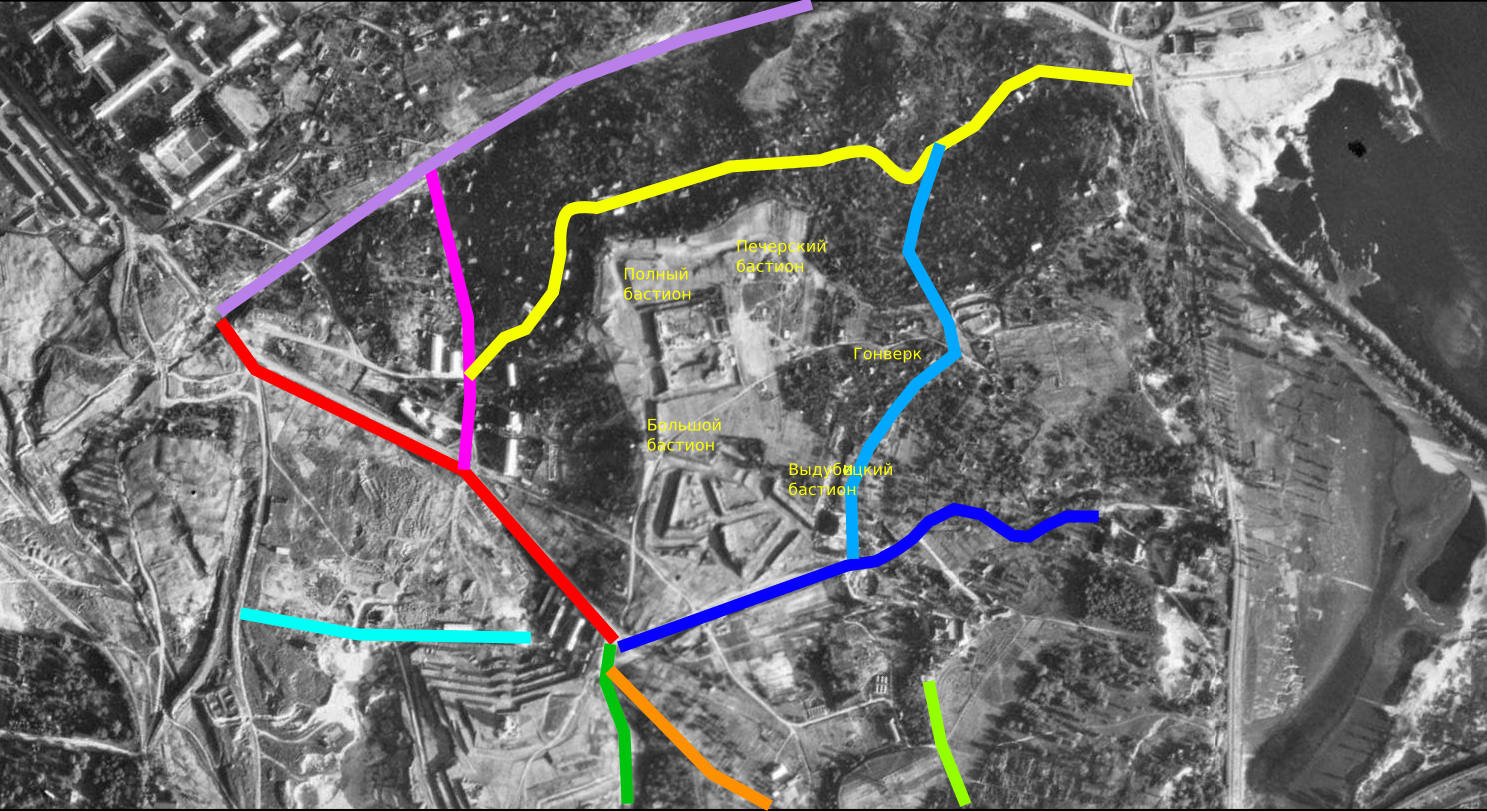
\includegraphics[width=\textwidth]{chast-vosp/zver/zver-krep-map-color.jpg}
\end{center}

Красная – улица Бастионная, прежде Святотроицкая. Она и теперь такая же.

Малиновая – улица Струтинского, она же Болсуновская. Сохраняет на этом отрезке прежнее положение.

Желтая – улица Мичурина, бывшая Лом\'аковская. Не изменилась.

Зеленая – начало Тимирязевской, совпадает с былой Омелютинской.

Оранжевая – ныне Кленовая аллея в ботсаду, прежняя Еврейская улица.

Салатовая – аллея от перекрестка под холмом с Ионинской церковью, низовье, начало бывшей Печерско-Кара\-ваевской улицы.

Синяя – аллея почти от входа в ботсад, до сиреневой аллеи, спуск по ней, и спуск к Выдубицкому монастырю. Это всё была улица Выдубицкая.

Голубая – Землянская улица. Теперь от нее остались: Землянская улица вне ботсада (примыкающая к Мичурина), и аллея над садом сирени, по краю хвойных.

Бирюзовая – улица профессора Подвысоцкого.

Фиолетовая – ныне бульвар Дружбы Народов, ранее Автострада.

Мы еще доберемся до Автострады, а пока сосредоточимся на основном холме Зверинца. По Святотроицкой на Выдубицкую, до нынешнего спуска Сиреневой аллеи, в 1909-1919 годах ходил трамвай номер 12. Это считалось Зверинецкой линией.

Она делилась на два участка. Данные за 1914 из справочника год таковы. Маршрут первого участка: Товарная станция (станция Протасов Яр, Бульонская, Лыбедско-Владимирская – Военное училище (перекресток Кутузова и Старонаводницкой). Второй участок: Старонаводницкая дорога, поселок Зверинец, Ионинский Свято-троицкий монастырь.

На плане того же года картина следующая. От товарной станции (что лежит напротив низовья Протасова яра через Лыбедь), маршрут таков: Бульонская, Лыбедско-Владимирская, Прозоровская дорога, по ней мимо Военного госпиталя, поворот на тогдашнюю Госпитальную (теперь это часть Леси Украинки), поворот на Большую Шияновскую (Лескова) на Печерский базар, оттуда по Петро-Могилевской на Кутузовскую, мимо Военного училища и войсковых бань, к Круглой башне №2 (Щорса, 44) и по прямой дороге (что уже существовала, ныне часть бульвара Леси) к месту Печерского моста (оврага под ним не было) и далее по Святотроицкой-Бастионной наверх.

В 1930-е по начало войны, Зверинецкую линию на короткое время восстановили, не делая поворот к Выдубичам, но от верха (у современного входа в ботсад) пустив по Зверинецкой, затем на Теличку, огибая юг ботсада, пересекая железную дорогу и далее на юг, восток между Бусовой и Лысой горами и по мосту через Лыбедь у подножия Лысой горы (где сейчас эстакада у низовий улицы Киквидзе).

Трамвайный маршрут на окраину Зверинца был обусловлен притоком паломников в Ионинский монастырь. Его строениям, как и Выдубицкому монастырю, порядком досталось во время взрыва 1918 года.

Пишу «взрыв», а точнее говорить – несколько, множество взрывов, и распространившиеся пожары.

Первые данные были – погибли 35 человек, 68 тяжело ранены, легко ранены 392. Через несколько дней цифры изменились, хотя, как предполагают исследователи, были весьма преуменьшены. Около 200 погибших. Разрушено 900 домов. 12000 человек в одночасье лишились крова.

Особо пострадали усадьбы на Свято-Троицкой, в Свято-Троицком переулке (Бастионный переулок), Печерской улице (от круглой башни по бульвару Леси Украинки до улицы Верхней), Ломаковской, Болсуновской,  Болсуновском переулке (часть нынешней Мичурина), Кургановской улице, Кургановском переулке, Церковной улице (сейчас Верхняя), Церковном переулке (переулок Верхний), Сафроновском переулке (теперь не существует).

Силы взрывной волны хватило, чтобы в центре, в Университете вылетели все стекла, а парадную дверь сорвало с петель. Большая волна пошла Днепром, опрокинув несколько лодок.

В том же году, комиссия по расследованию выработала две основные версии пожара и взрывов на артиллерийских складах. 

По одной, часовой взялся чинить ящик с сигнальными ракетами. 

По другой, начался пожар в сарае номер 3, с архивом старых документов. И когда солдаты разбирали эти добро, ища источник возгорания, то вытащили фугас. Он сразу взорвался. После воспламенился сарай с сигнальными ракетами, они стали разлетаться во все стороны и поджигать другие деревянные сараи, где хранилась взрывчатка, а также навесы над штабелями снарядов.

   Сразу после конца света на Зверинце, правительство Скоропадского быстро озаботилось возведением здесь, на месте смерти и разрушения, правительственного района. Но строительство отложилось благодаря исследованию подземных пустот. А затем и власть переменилась.

   А представьте, если бы решение о строительстве утвердили до взрыва? Пришлось бы убеждать жителей отселяться, выплачивать им деньги гораздо б\'ольшие, нежели дали погорельцам, да и затраты на само разрушение зданий... Взрыв решил много трудностей на пути к решению задачи.

После него, местом артиллерийских складов и стал Лысогорский форт, а Зверинецкий пребывал в запустении до сооружения ботанического сада. 

А жизнь не ушла оттуда, но продолжилась даже в самой близости к пеклу, на улице Мичурина, тогдашней Ломаковской. Ломаковская была козырной, мощёной. Возродились Болсуновская до перекрестка с Бастионной-Святотроицкой,  оттуда пополз частный сектор наверх к нынешнему входу в ботсад...

Скуден набор фотографий, запечатлевших уничтожение всего сущего 5 июня 1918 года. Некоторые сделаны немцами, с аэроплана и земли. Приведут некоторые снимки. Более подробный разбор читайте в отдельной моей книге «Зверинецкий форт», где заодно поднимаются темы, освещенные тут лишь вкратце.

\newpage

\begin{center}
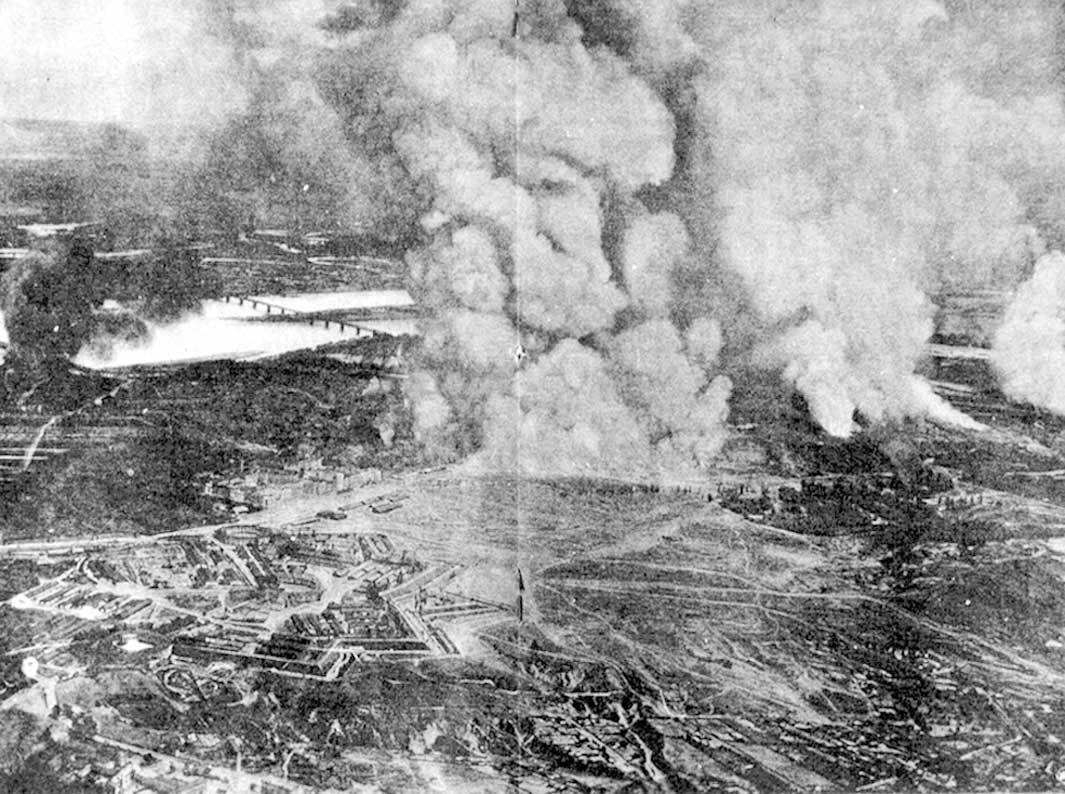
\includegraphics[width=\textwidth]{chast-vosp/zver/boom02.jpg}
\end{center}

Звездообразно очерченная цитадель в левой нижней четверти фотографии – Васильковское укрепление. Большей частью оно сохранилось. Выделяются его круглые башни. Номер 2, восточная – на бульваре Леси Украинки напротив новостроек Царского села (Щорса, 44/Леси Украинки 26-В), номер 3, Прозоровская – у перекрестка улиц Щорса с Кутузова (Прозоровская башня). Бублик восточной\footnote{50°25'27.81"N 30°32'29.05"E} хорошо виден на фотке. В середине кадра, очаг дыма – примерно там, где сейчас улица Бастионная на отрезке от пересечения с улицей командарма Каменева и Печерским мостом. Конечно, это уже пожар – взорвалось ведь в другом месте, в нынешнем ботсаду. На фотографии, там где сейчас Суворовское училище (оно же имени Богуна) – чуть выше бублика – постройки Алексеевского инженерного училища. Мост через Днепр – Неводницкий. Странно, что область, где пожары и взрывы довольно четко ограничена только Зверинцем.

Вот еще несколько фотографий. За клубами дыма гибнут люди. Искореженные орудия войны. Поваленные заборы.

\newpage
\vspace*{\fill}
\begin{center}
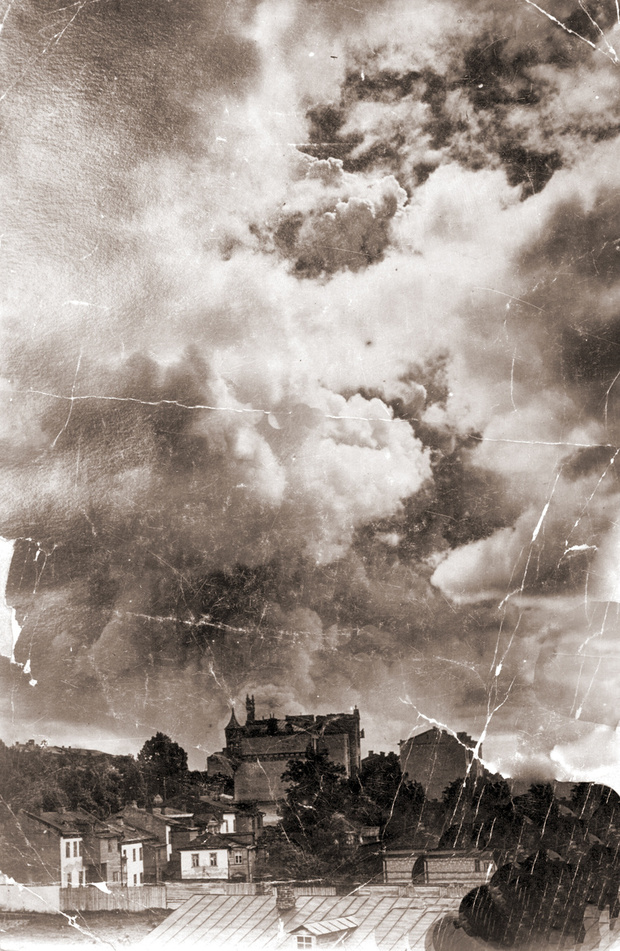
\includegraphics[width=\textwidth]{chast-vosp/zver/vzryv.jpg}
\end{center}
\vspace*{\fill}
\newpage

\vspace*{\fill}
\begin{center}
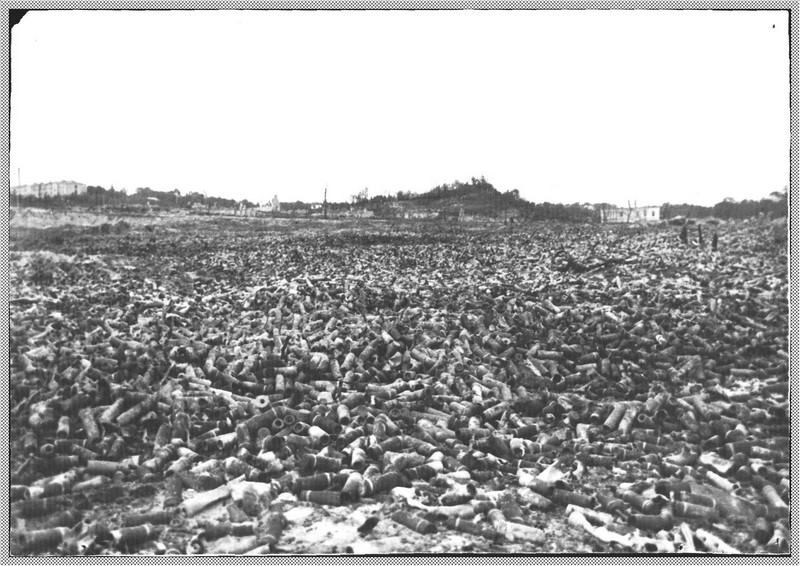
\includegraphics[width=\textwidth]{chast-vosp/zver/vz001.jpg}
\end{center}

\begin{center}
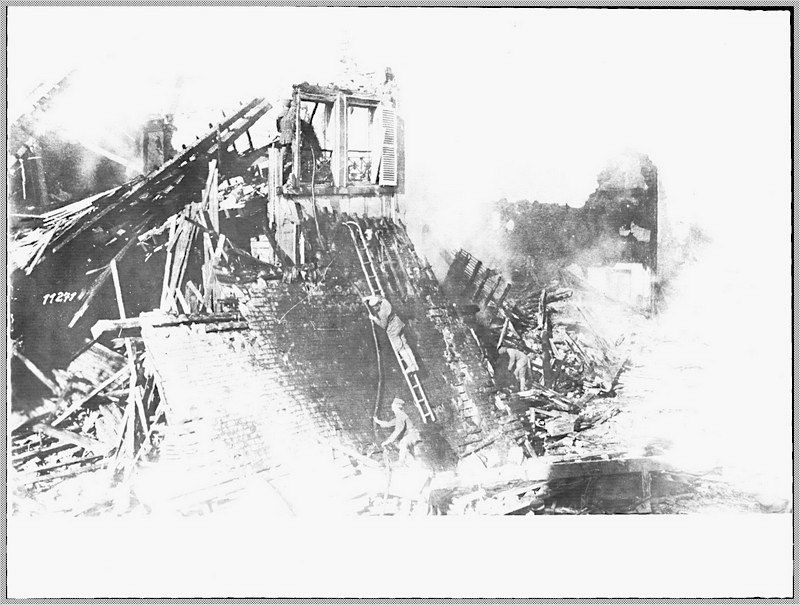
\includegraphics[width=\textwidth]{chast-vosp/zver/vz002.jpg}
\end{center}
\vspace*{\fill}

\newpage

\vspace*{\fill}
\begin{center}
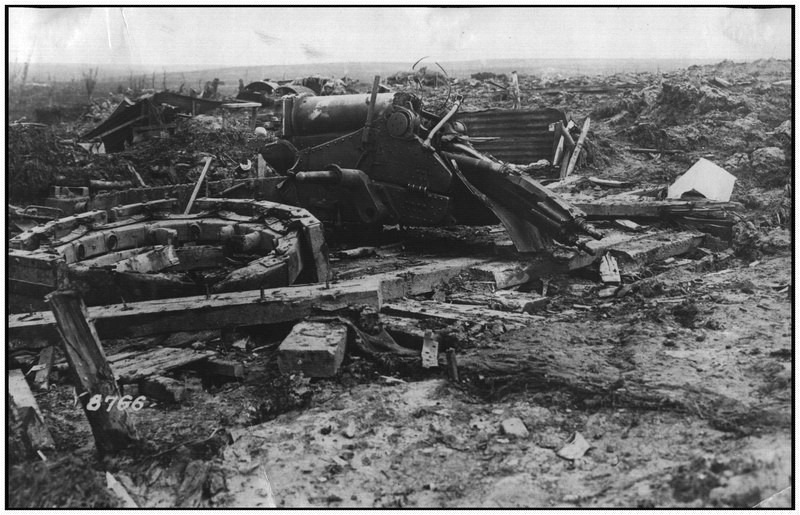
\includegraphics[width=\textwidth]{chast-vosp/zver/vz003.jpg}
\end{center}

\begin{center}
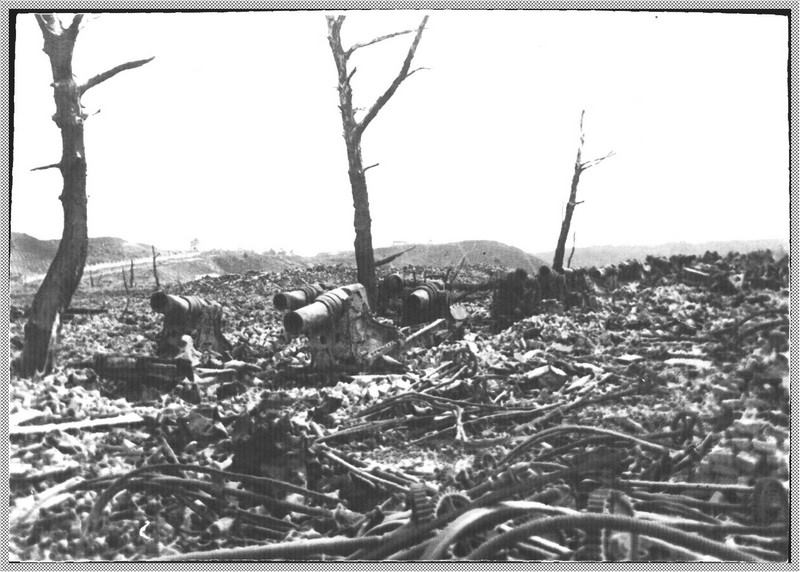
\includegraphics[width=\textwidth]{chast-vosp/zver/vz004.jpg}
\end{center}
\vspace*{\fill}

\newpage

\vspace*{\fill}
\begin{center}
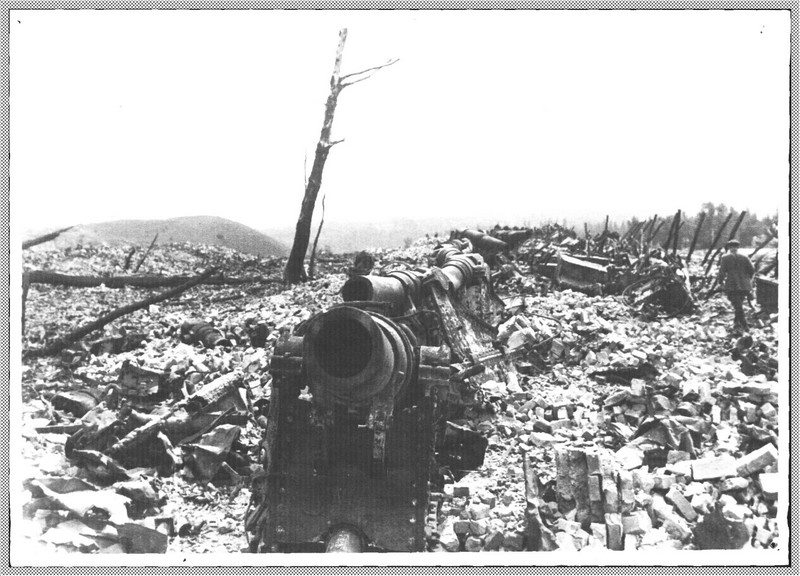
\includegraphics[width=\textwidth]{chast-vosp/zver/vz005.jpg}
\end{center}

\begin{center}
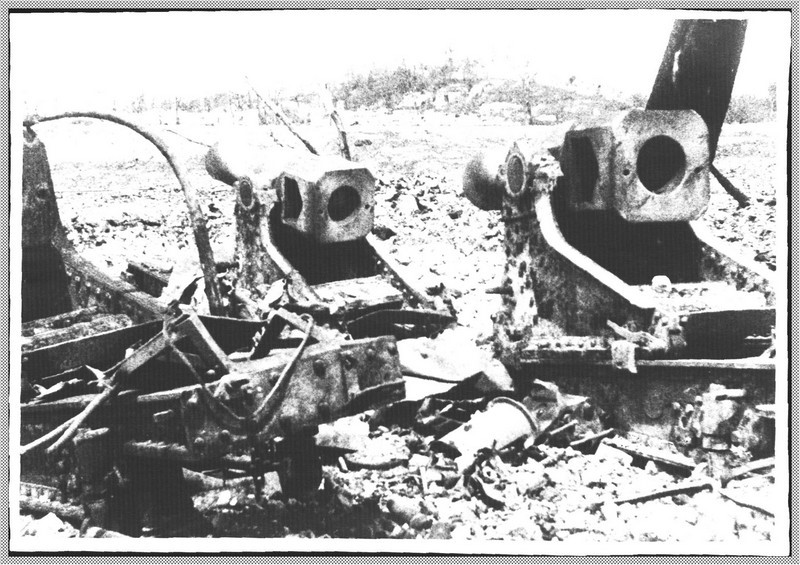
\includegraphics[width=\textwidth]{chast-vosp/zver/vz006.jpg}
\end{center}
\vspace*{\fill}

\newpage

\vspace*{\fill}
\begin{center}
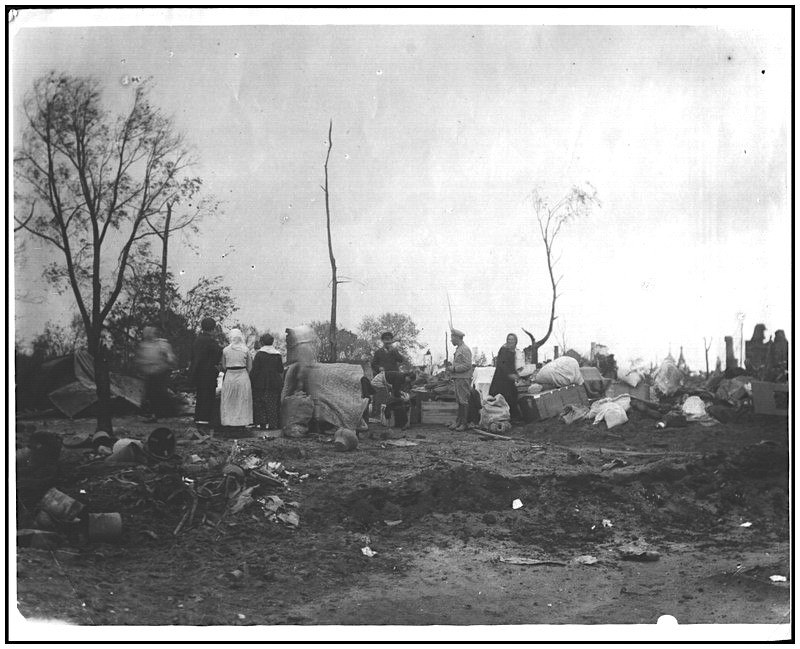
\includegraphics[width=\textwidth]{chast-vosp/zver/vz007.jpg}
\end{center}

\begin{center}
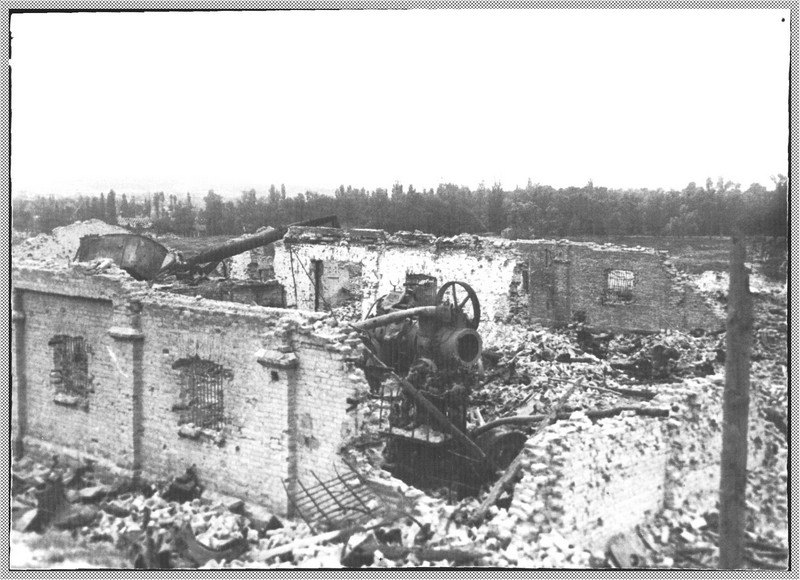
\includegraphics[width=\textwidth]{chast-vosp/zver/vz008.jpg}
\end{center}
\vspace*{\fill}

\newpage
\vspace*{\fill}

\begin{center}
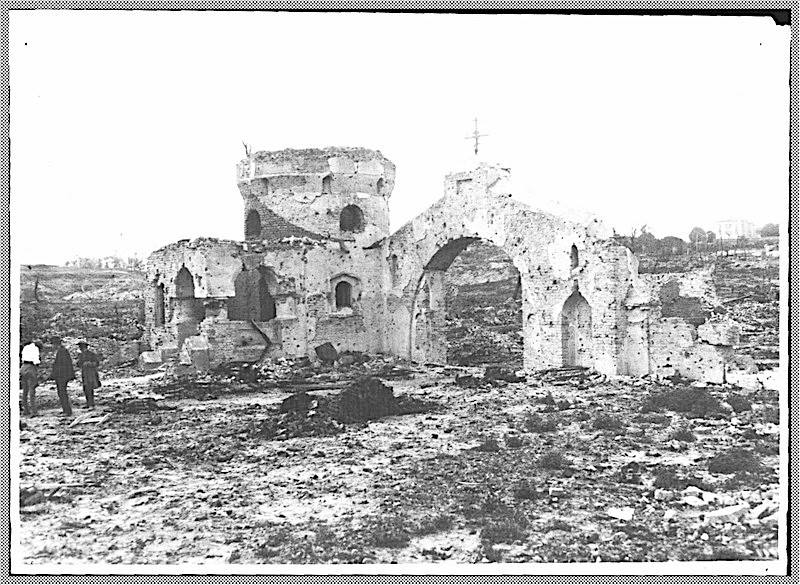
\includegraphics[width=\textwidth]{chast-vosp/zver/vz009.jpg}
\end{center}


\begin{center}
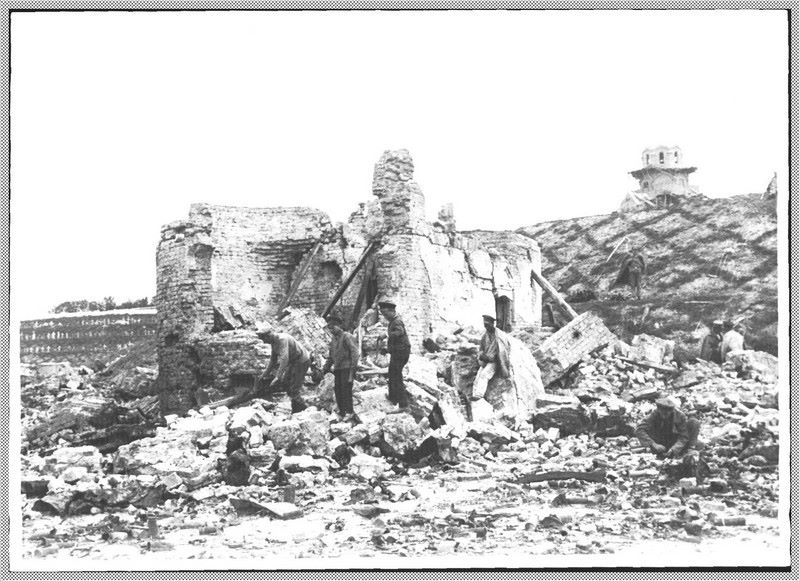
\includegraphics[width=\textwidth]{chast-vosp/zver/010.jpg}
\end{center}
\vspace*{\fill}

\newpage
\vspace*{\fill}

\begin{center}
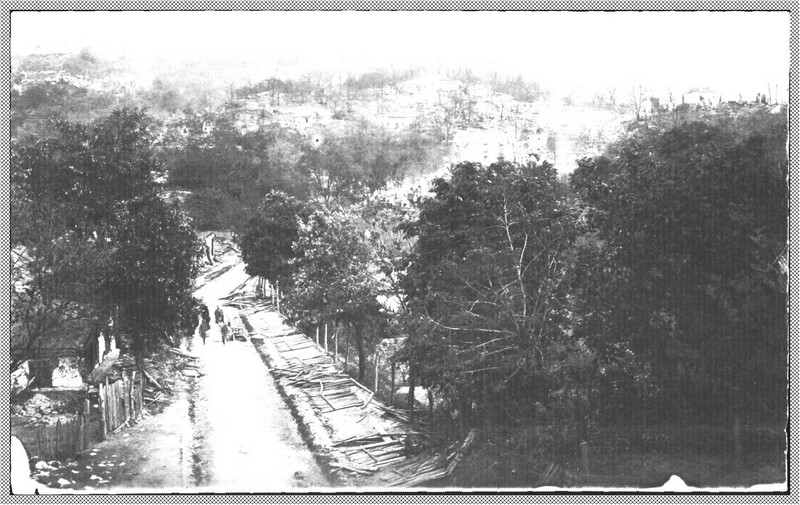
\includegraphics[width=\textwidth]{chast-vosp/zver/011.jpg}
\end{center}

\begin{center}
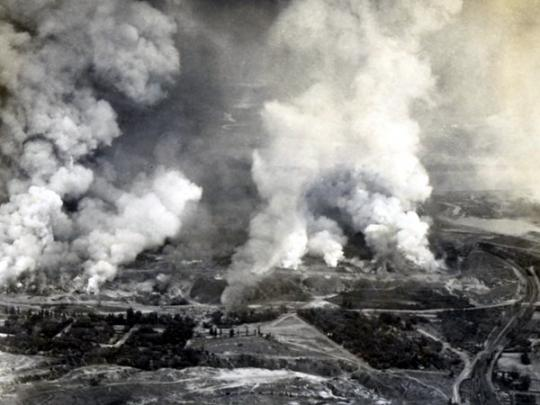
\includegraphics[width=\textwidth]{chast-vosp/zver/013.jpg}
\end{center}

\vspace*{\fill}

\newpage

\vspace*{\fill}


\begin{center}
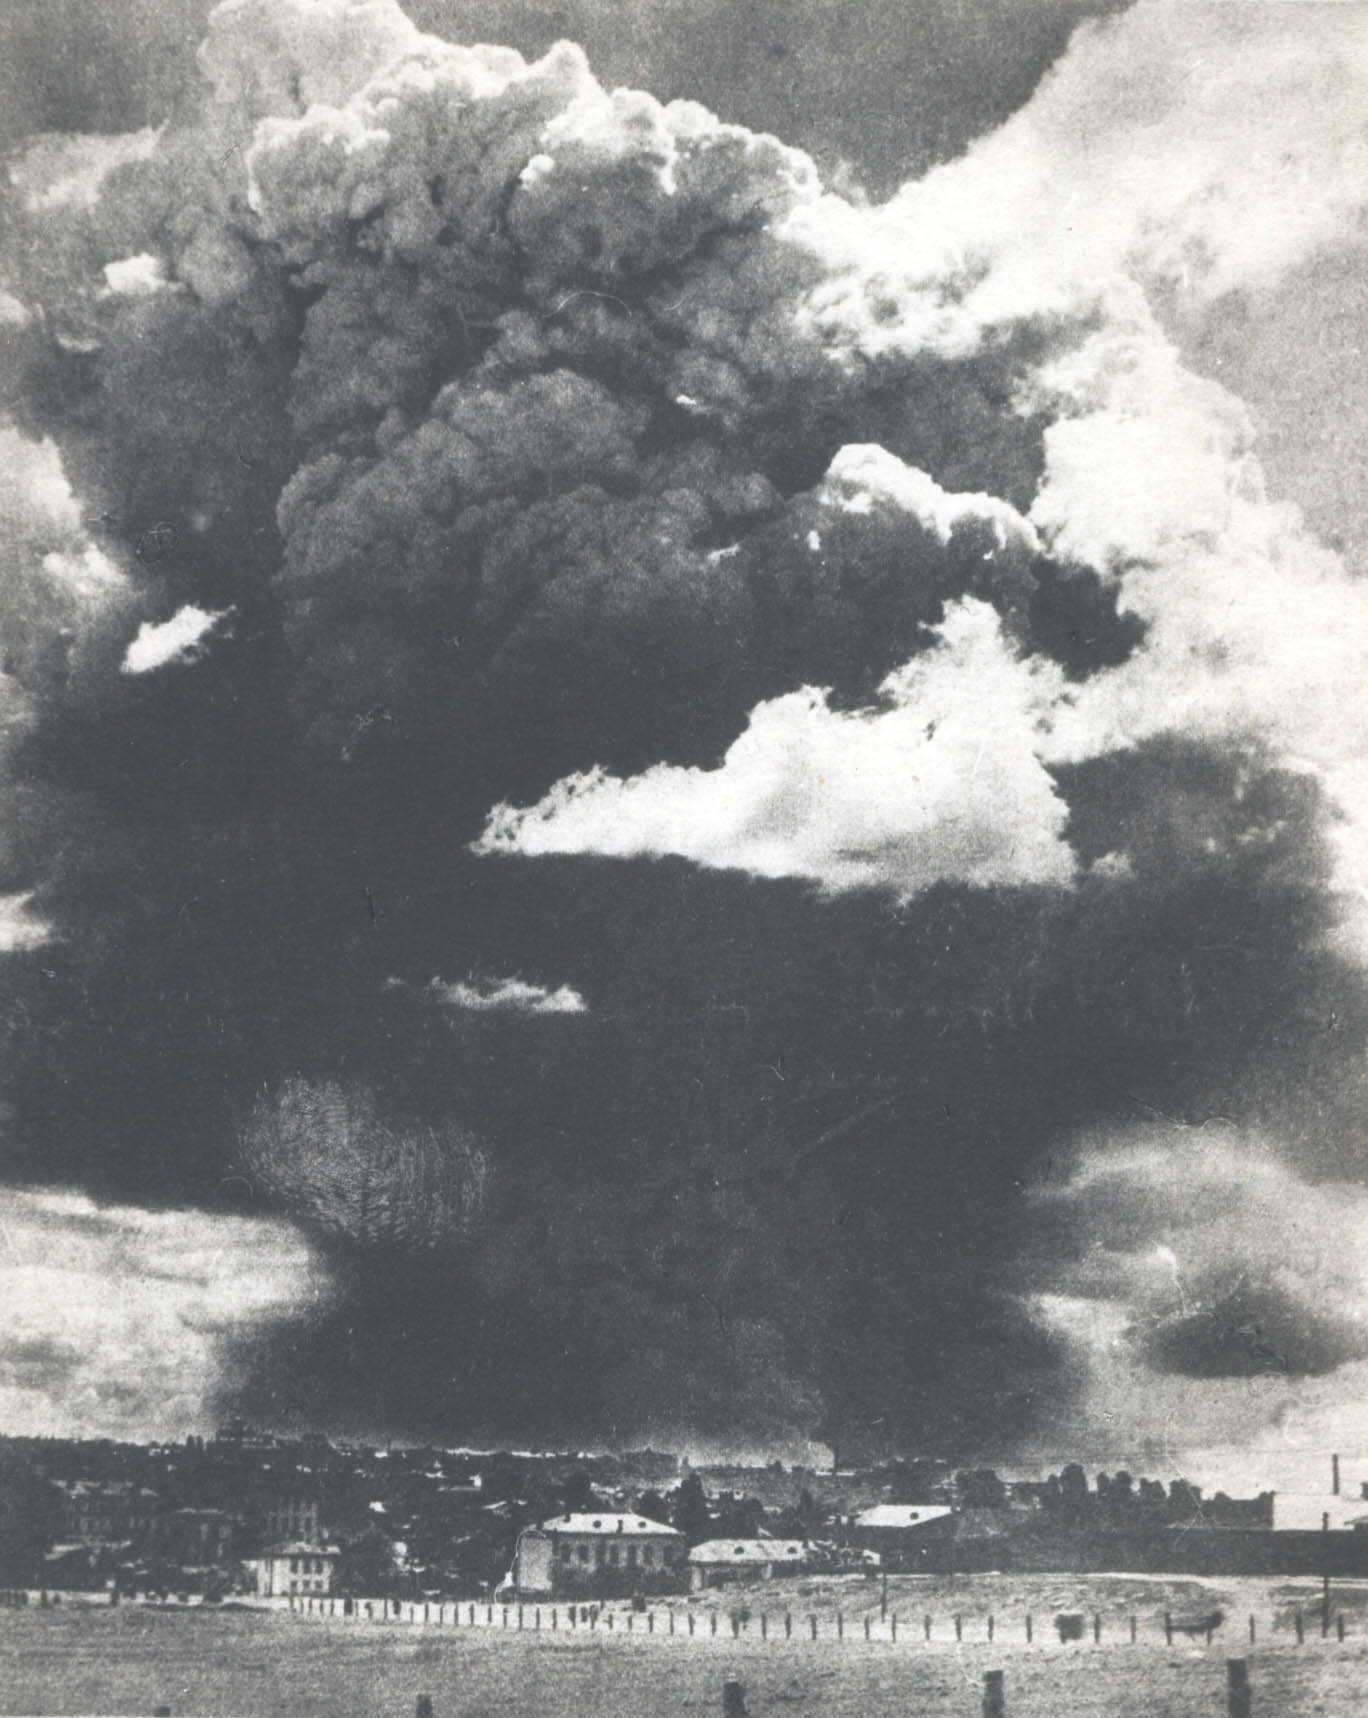
\includegraphics[width=\textwidth]{chast-vosp/zver/zverinec_vzryv-1918.jpg}
\end{center}

\vspace*{\fill}

\newpage

\vspace*{\fill}

\begin{center}
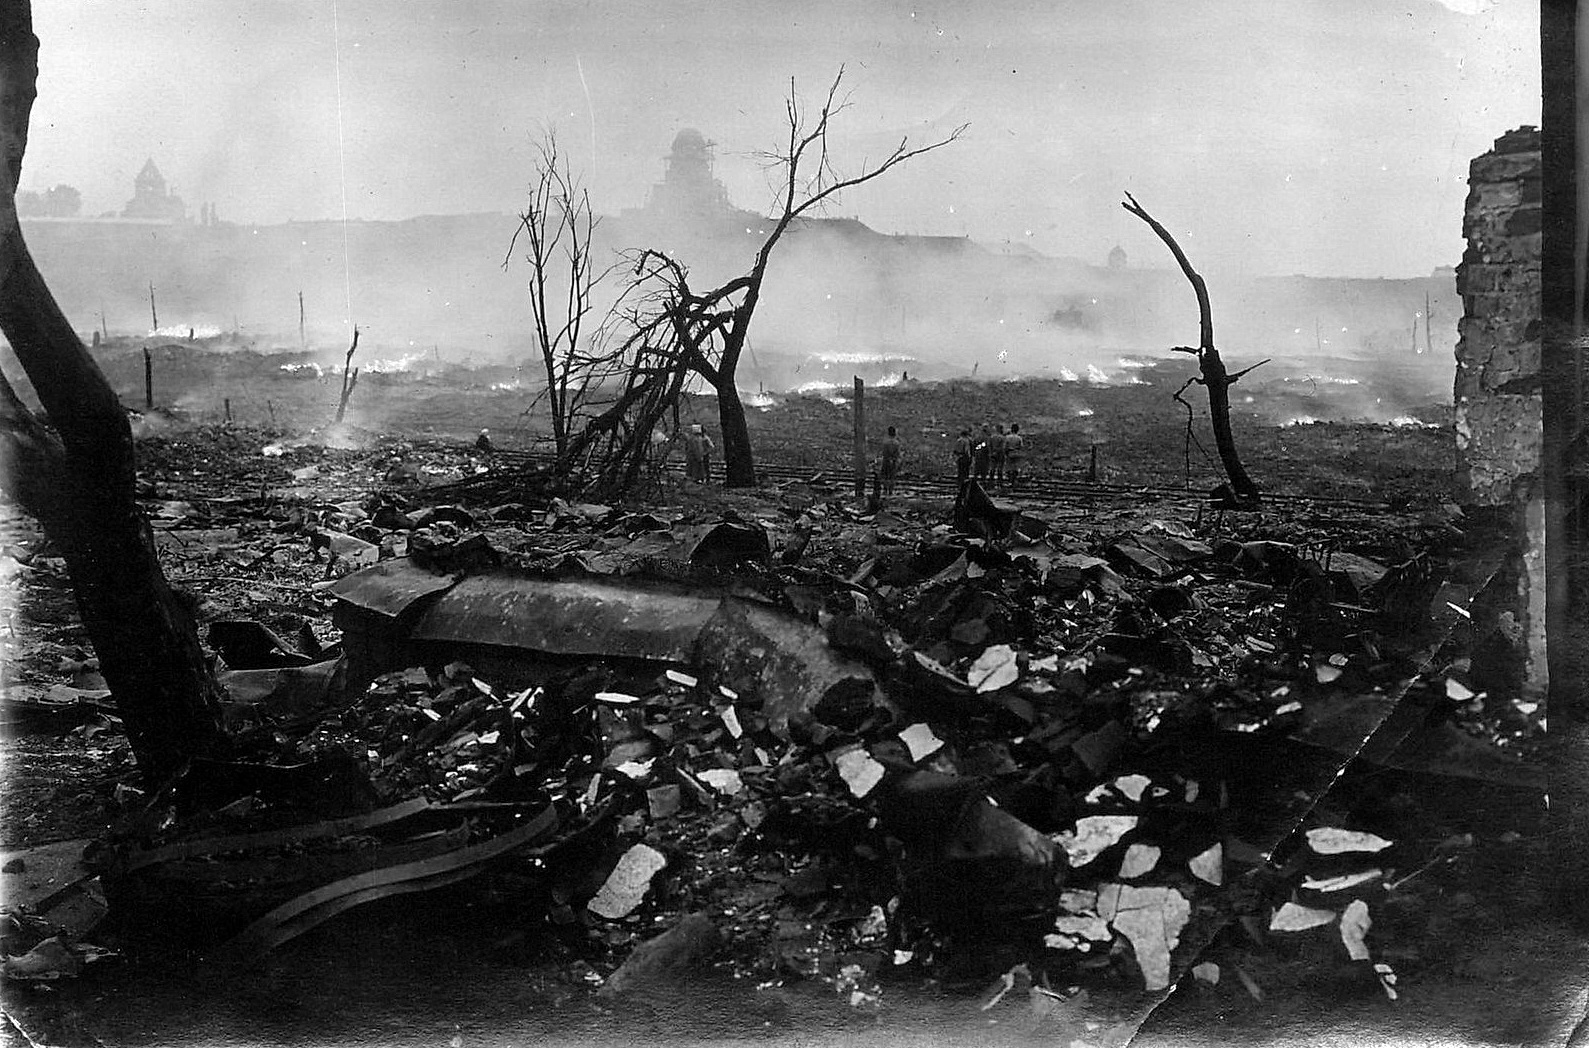
\includegraphics[width=\textwidth]{chast-vosp/zver/1350612.jpg}
\end{center}

\begin{center}
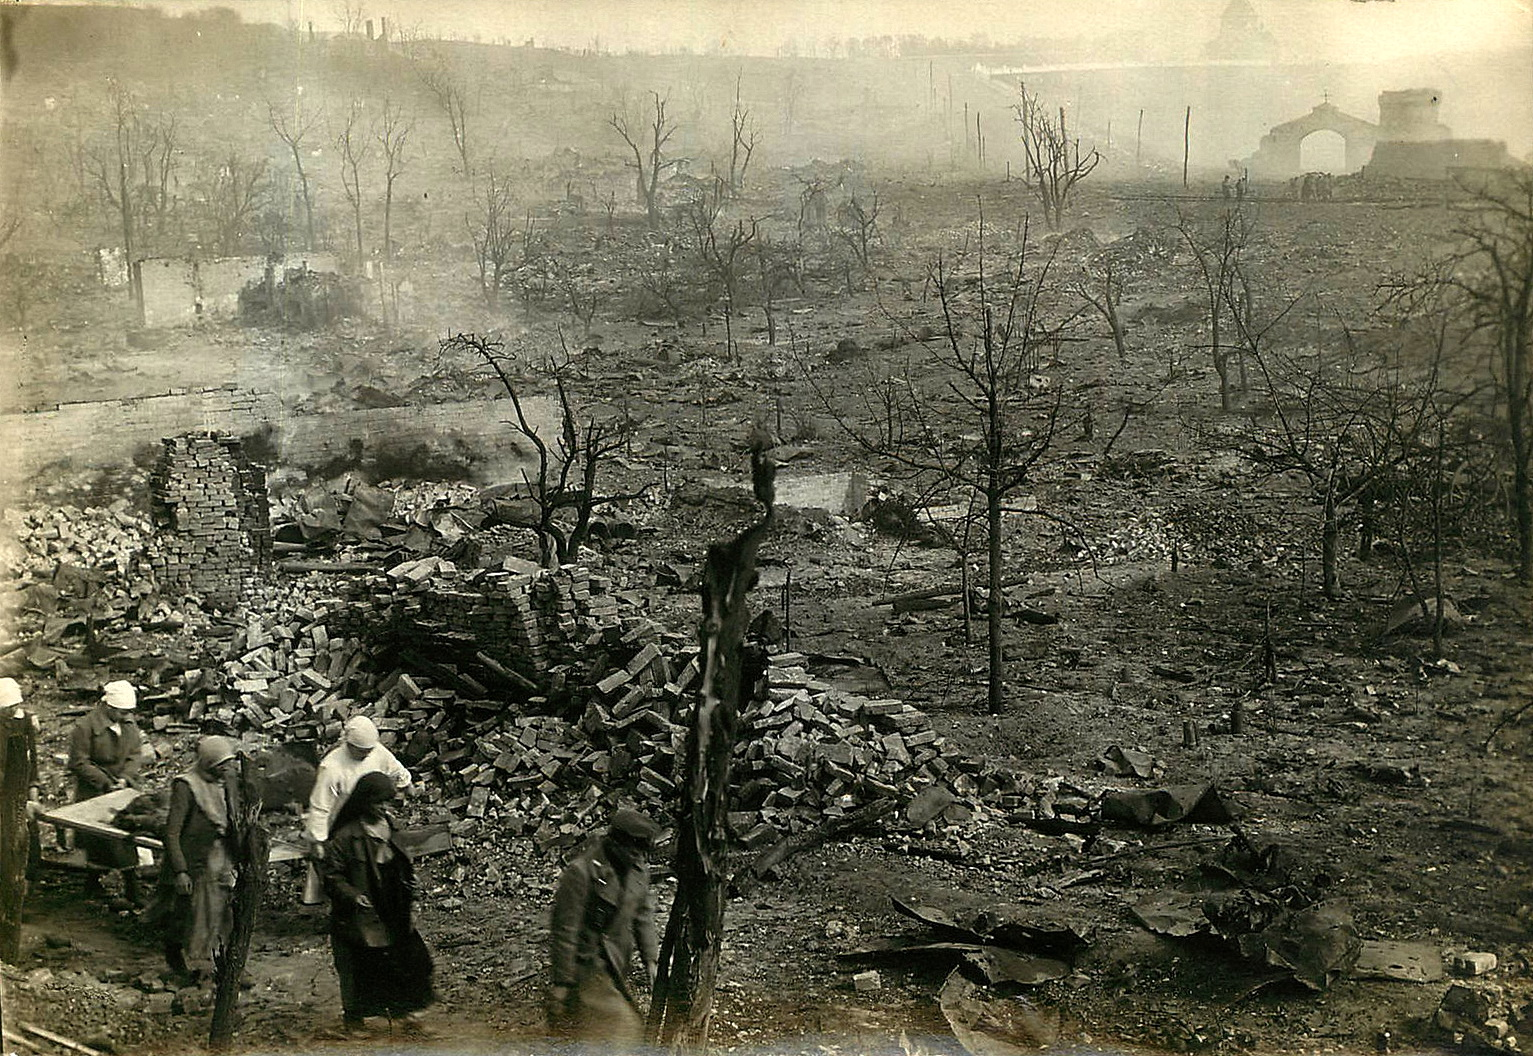
\includegraphics[width=\textwidth]{chast-vosp/zver/1350615.jpg}
\end{center}

\vspace*{\fill}

\newpage

\begin{center}
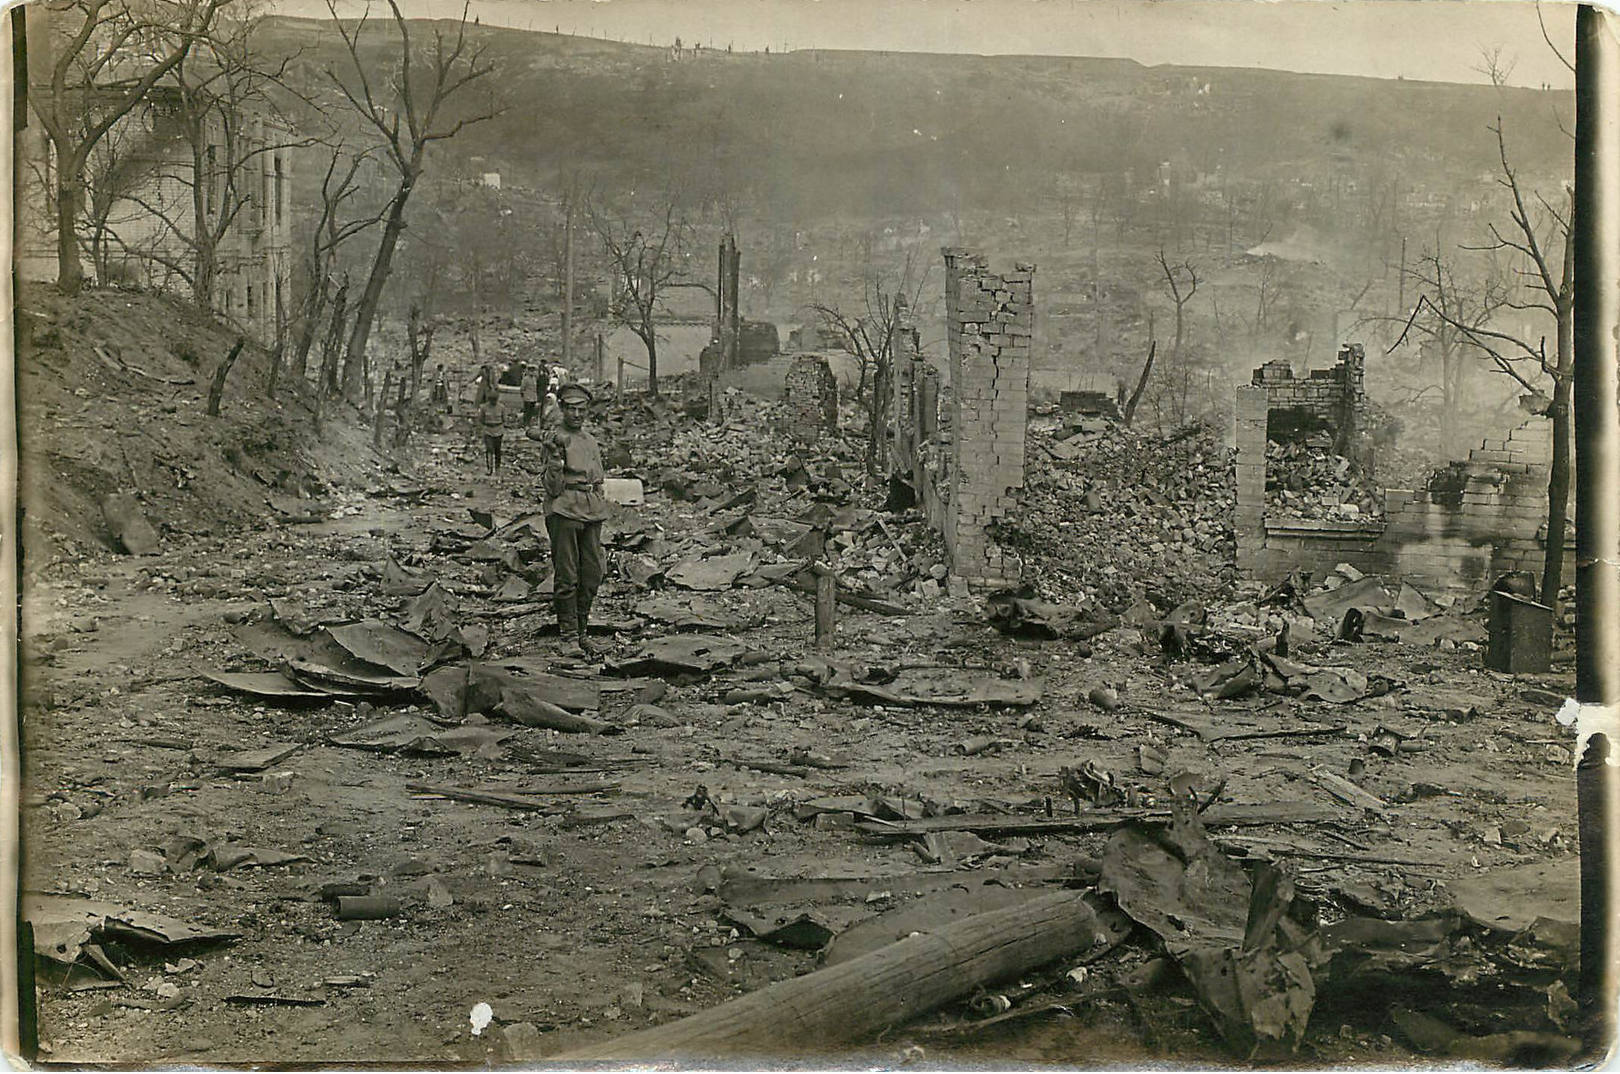
\includegraphics[width=\textwidth]{chast-vosp/zver/902_001.jpg}
\end{center}


Взрывам 1918 года на Зверинце историками уделено еще меньше внимания, чем «Куренёвской трагедии», хотя редко и мало где происходило подобное. Ни памятного знака, ничего – лишь разрозненные очерки краеведов. Изгибы земляных валов в ботсаду напоминают ныне живущим – но лишь тем, кто знает их прошлое – о былом.

Напротив входа в ботсад, через площадь – Институт проблем прочности. Здесь и на примыкающем склоне в сторону улицы Подвысоцкого, да внизу, в низине с западной части Бастионной, к 1915 году устроили Братское кладбище, где хоронили погибших в Первой Мировой войне. Занимало оно треугольный квартал, ограниченный по сторонам улицами Бастионной, Катерины Билокур, профессора Подвысоцкого. Институт, овощной, культтовары, детсад, задворки 88-й школы – всё это было отведено под кладбище. Поныне склоны ниже института взяты могильными террасами, в коих оборудованы погреба жильцов из хрущовок на улице Подвысоцкого.

При разбивке кладбища, местность преобразовали в согласии с представлением, что террасы олицетворяют шеренги. В конце каждой погребали «старшину». В 1916-м, торжественно, при участии матери царя – императрицы Марии Федоровны, разных важных генералов и высоких церковных чинов, заложили храм-памятник Николая Чудотворца. Солдатиков хоронили-закапывали, церковь начали строить да не завершили – грянула революция.

\begin{center}
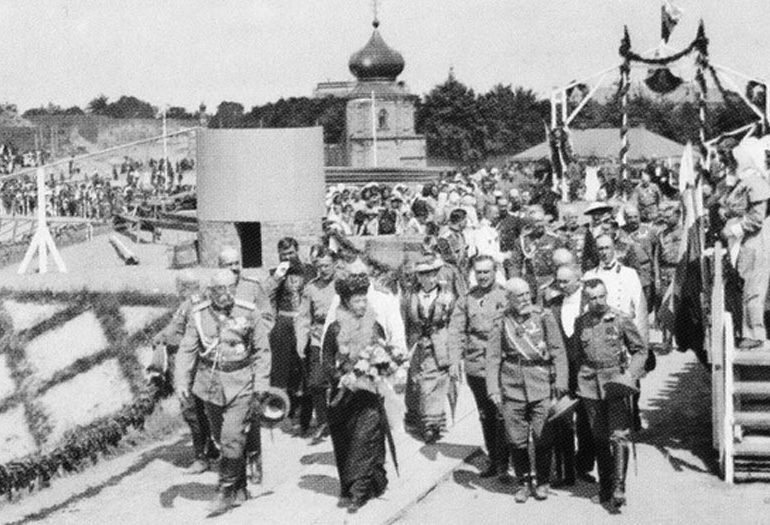
\includegraphics[width=\textwidth]{chast-vosp/zver/brat-zakl.jpg}
\textit{1916. Торжественное заложение храма на Братском кладбище.}
\end{center}

Ближе к 1930-м бесхозное кладбище служило никому не нужным памятником никому не нужным жертвам. Местные жители растащили все деревянные кресты на топливо, кто-то разрыл часть могил, и валялись средь них солдатские кости. На плане 1923-30 годов показаны захоронения лишь в той части, где сейчас удолье детсада и склон над ним. Точно напротив «моего» переулка. На плане отмечены сохранившиеся на то время могилы? Или же с момента открытия кладбища по тридцатые хоронили только на том участке?


% Ваня, а ты где погиб? Там-то. А душу не греет, что для праха твоего валы шеренгами выстроили, да генералы с огромными усищами радели памятник, церковь поставить – не греет? Нет, не греет. А знаешь, где теперь генералы с усами царскими? Знаю, в Париже, мемуары пишут. А что ж так получилось – ты здесь череп оскалил, они в Париже себя холят, а ведь на одной войне сражались? Да вот, постояли за царя и отечество.

В 1935 году кладбище хотели использовать по назначению, для упокоения всех граждан, не только военных, а недостроенную церковь превратить в крематорий, однако почин не поддержали свыше.

Так и стояло одичавшее кладбище с развалинами церкви, покуда в 1953 году на него, точнее на прочные стены храма, не положил глаз будущий академик Георгий Сергеевич Писаренко\footnote{В восьмидесятых он кроме прочего был руководителем общественно-научной организации по изучению непознанных явлений. Похоронен на Зверинецком кладбище.} из Института металлокерамики и специальных сплавов. Вскоре институт получил участок кладбища, а в помещении церкви обустроили лабораторию. Она и новые корпуса легли в основу образовавшегося в конце шестидесятых Института проблем прочности.

Под горой с институтом проходит улица Подвысоцкого и окончание четной части Бастионной. Там было несколько магазинов и, в угловом доме подле детсада – детская кухня, где для грудничков бесплатно давали разные каши в бутылочках и фруктово-молочное пюре. Кухни больше нет и даже крыльцо её разобрали. В низину я сходил крутым земляным склоном. Лучше, чем тратить время и топать к лестничке или пользоваться тропкой мимо сетчатой ограды детсада (она проходит, как теперь понимаю, четко по границе былого кладбища).

Помню, в детстве, годика четыре мне было, иду по Бастионной над этим удольем, и вижу младенца, частично скатившегося по горе так, что пеленки размотались. И некая девочка в свитере, постарше, его оттуда достает. Она попросила ей помочь, мы достали младенца, что потом – забыл. Много позже, я никак не мог объяснить себе случай, пока не узнал про взрыв в 1918 году. Я повстречал призраков? Как ни крути, гиблое место. И никто об этом не помнит.

...Там внизу меня больше всего привлекал магазин «Культтовары», на первом этаже дома. Отдел справа с игрушками, слева с канцелярскими товарами, и посередке кажется диафильмы и проекторы. За кассой сидел парализованный Володя, единственный мужчина в магазине, так были всё продавщицы.

Рядом находились, в такой же хрущовке, хлебный и молочно-колбасный магазины. Летом 2013 года все они были совмещены в один большой, но закрытый магазин по продаже окон. Я очень четко помню обстановку хлебного и молочки, запах, звук, грузовик «ГАЗ», подвозивший свежий хлеб.

Если пройти оттуда дальше, мимо детсада, то в полуяме под Институтом проблем прочности тоже стоят хрущовки, а долгая лестница карабкается мимо голубятен\footnote{К 2017 сгинули.} наверх к развороту у ботсада, и в первом доме около лестницы, внизу, был чудесный магазин «Художественная самодеятельность», просуществовавший примерно до начала века нынешнего. 

\begin{center}
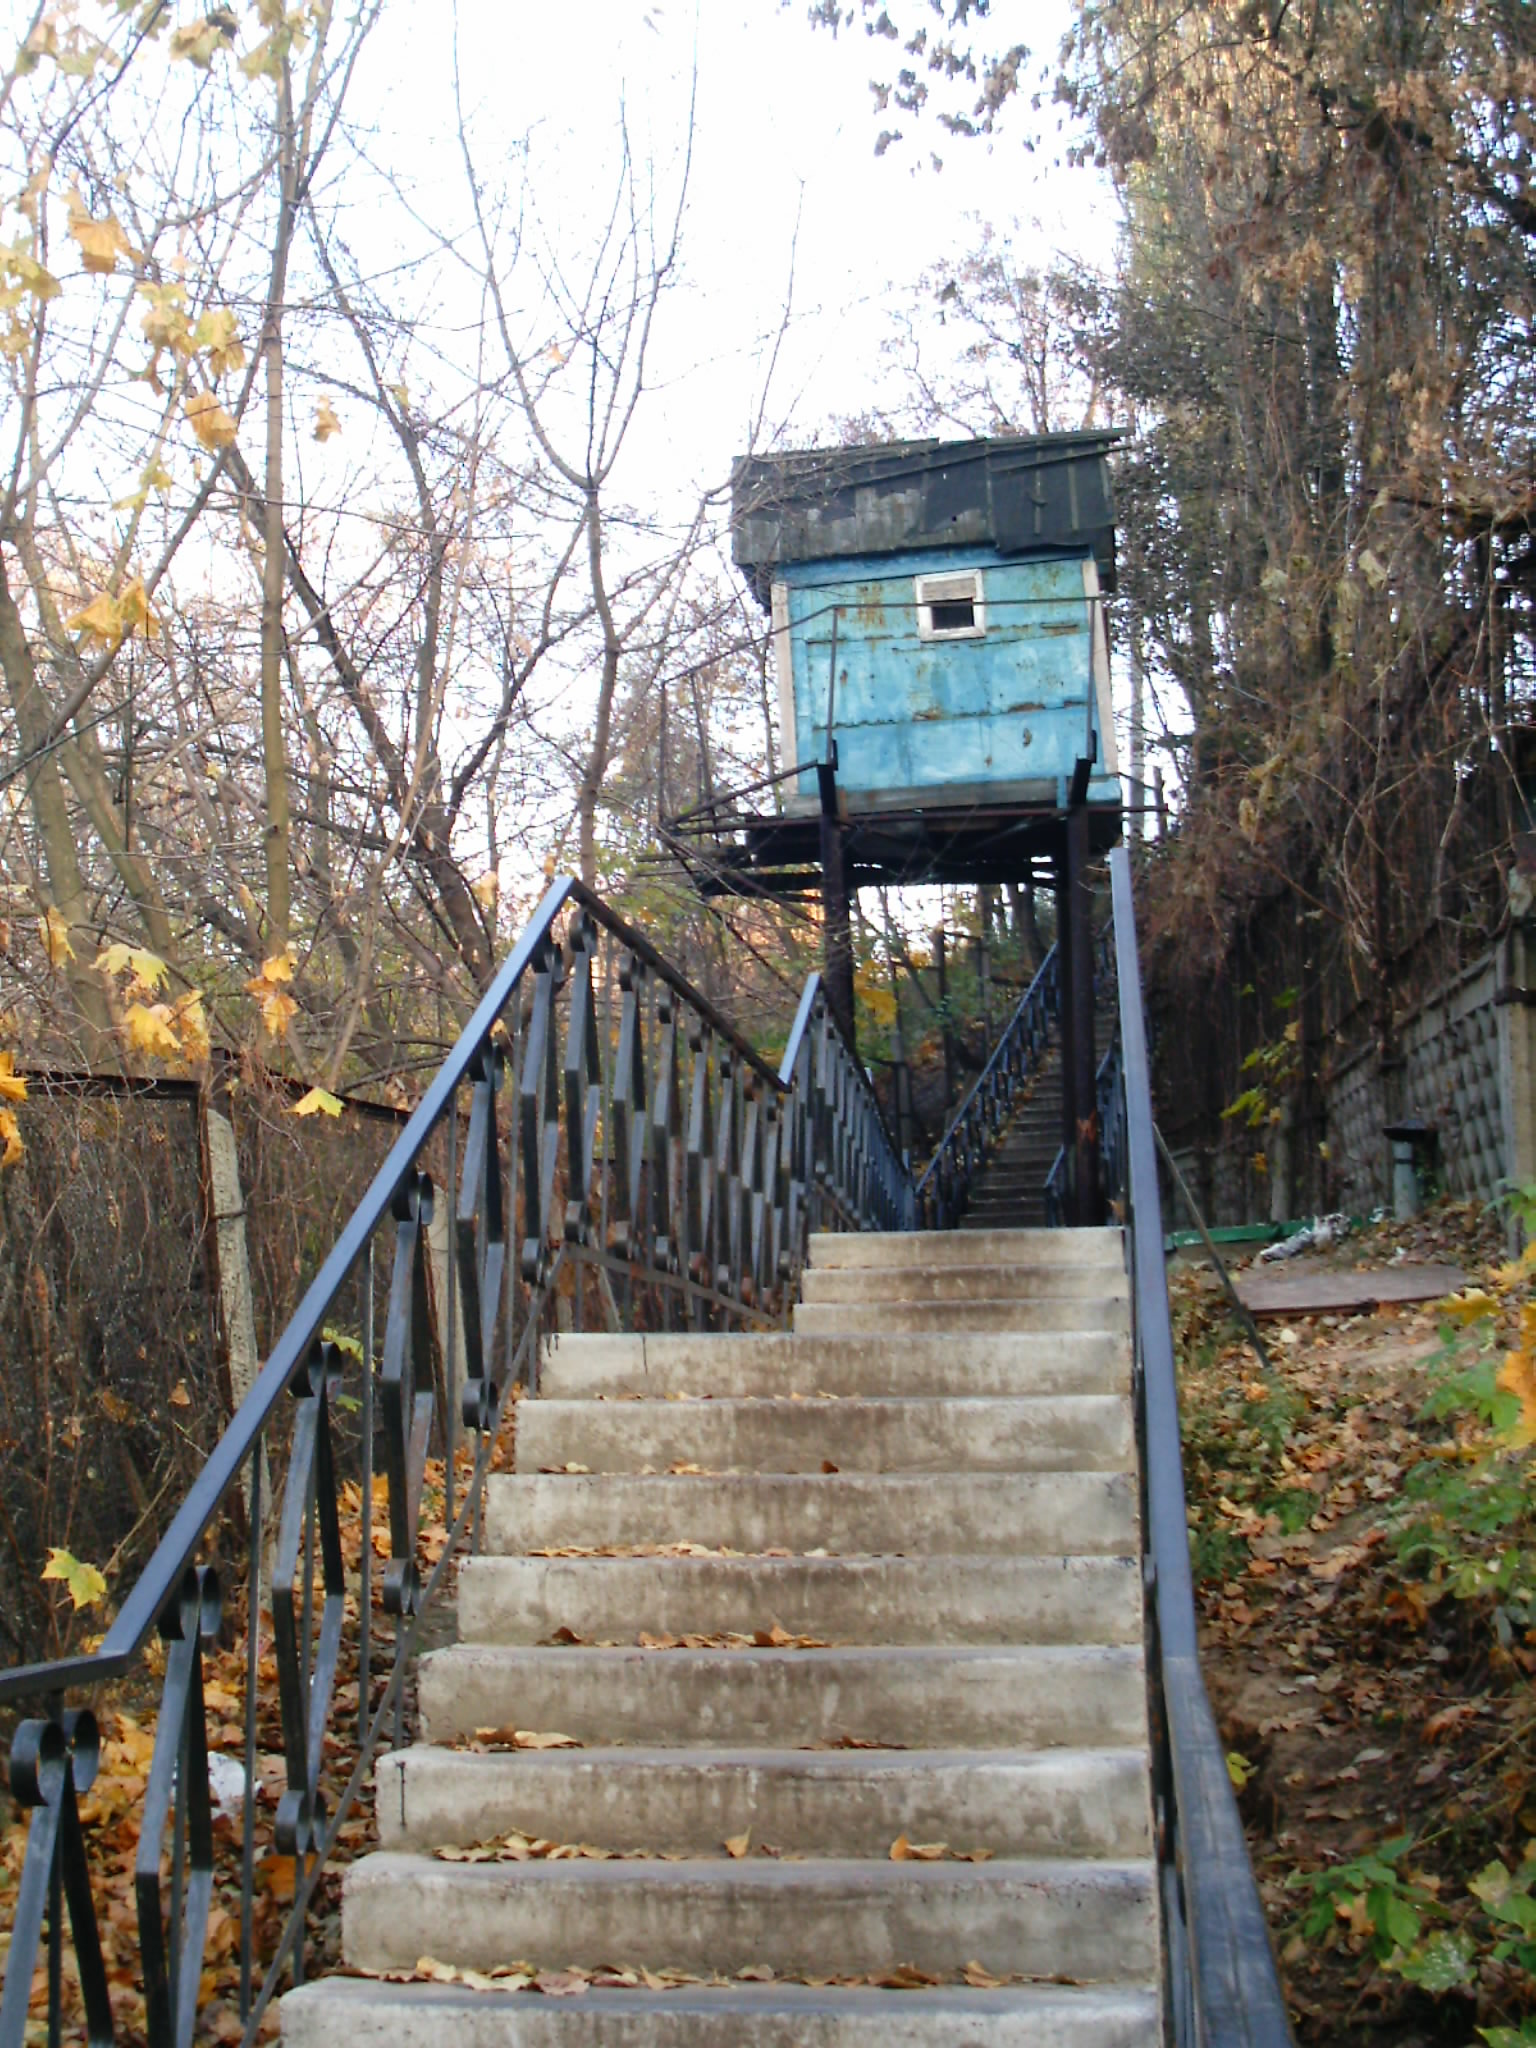
\includegraphics[width=0.80\textwidth]{chast-vosp/zver/imag0017.jpg}

\textit{2005 год. Лестница.}
\end{center}

\newpage

Я всегда заходил туда больше чтоб посмотреть, не купить. Мы там купили только одно – белую собачку Тяпу – куклу, одевающуюся на руку. Нынче сюда бы повалили создатели любительского кино и музыканты с уклоном в квартирники. 

В «Самодеятельности» продавалось всё – грим, парики, народные костюмы, баяны, балалайки, куклы для спектаклей, струны, гитары, бубны, дудки, накладные косы, черт знает что еще, не помню. 

В последний раз, когда я видел вывеску этого магазина, его помещение уже предназначалось для иных целей, вовсю шел ремонт, а дверь охранялась письменным столом, невесть с какой целью вынесенным наружу.

За домом под гору вьется лестница, чередуясь с тропой между погребами. Они выкопаны в кладбищенской земле! Затем слева – сетчатый забор детского сада, справа – неперелазная ограда Института проблем прочности. И лестница. И голубятня, испокон веков нависающая над прохожими. 

В одно из своих посещений родины, «неузнанный, невидимый», я бродил там и повстречал на лестнице старика, которого помню с самого детства. Сей уже тогда седой дедушка, был, как тогда говорилось, «щирый украинец» – с усами, резной палкой, словно сошедший со страниц записок Яворницкого. Он всегда в шутку говорил, что из меня будет «великий танцюрист» – я до школы занимался в кружке танцев. 

Как сообщил мне позже Виталий Хропко, этот дедушка жил в последнем подъезде дома на Подвысоцкого, 20, и умер примерно в 2016 на 92-м году жизни. Ходил в «Баклажан» (бывший «Овощной»), во дворе декламировал на память поэзию Шевченко. Во время войны был ранен в ногу. Работа его была как-то связана с железной дорогой.

И вот смотрю, уже ведь много лет прошло – он спускается мимо, ничуть не изменился, только уже один, а то с супругой раньше ходил. Меня, понятно, не узнал. Островок моего прошлого.

Я сейчас снова мысленно вылез к ботсаду – самой верхушке холма, где грибы-навесы над кассами и была конечная троллейбуса номер 14. 

\begin{center}
\includegraphics[width=\linewidth]{chast-vosp/zver/imag0027.jpg}

\textit{Снимок 2005 года.}
\end{center}

Если чуть спуститься отсюда Тимирязевской и свернуть на Зверинецкую, то напротив дома номер 4, хрущовки, где жила конь-собака породы ирландский волкодав, на месте теперешнего терема был разворот-отстойник 62-го автобуса. Ходили такие темно-желтые «Икарусы». У ботсада они высаживали пассажиров, ехали вниз на разворот, а потом принимали пассажиров опять наверху. Подальше от любопытных глаз, водители автобусов сливали за деньги бензин подруливающим машинам частников.

Маршрут №62 сократили будто бы по просьбам жителей кооперативного дома 15 по Бастионной, которым мешал производимый автобусами шум, хотя в таком случае – почему не сократить 62-й до остановки возле школы? Нет же, перенесли аж до Печерского моста, точнее к самому началу забора Суворовского училища. Приходилось (говорю о восьмидесятых-девяностых) доезжать на 14-м троллейбусе и пересаживаться в автобус. В 21 веке 62-й маршрут снова продлили на Бастионную.

А 14-й троллейбус раньше ездил иначе, чем сейчас. Вторая конечная была на Бессарабке, возле школы. Но весь квартал к югу от рынка, со школой, жилыми домами и стрелковым тиром снесли и построили там торговые здания.

Вернусь к остановке у ботсада. Пойдем по Бастионной вниз. Улица имеет вид перевернутого коромысла, что вначале спускается от ботсада к перекрестку подле 133-й школы, а затем поднимается к перекрестку около Печерского моста.

Вот у зимнего, малого входа в ботанический сад начинается каменная стенка с металлическим забором. Через него просматривается орех, липы, домик туалета. В детстве я не шел по тротуару, а непременно залезал на стену. Потом тропка – уходит вверх, вдоль направившегося прочь забора, забор сменяется белым, высотным домом номер 15, за ним – мой родной проулок к домам 11 и 11-А, заросший по бокам сиренью. В эти кусты я летел вперед головой, когда великом со всей скорости наехал колесом на бровку.

В 13-м, тылом вкопанном в холм, Арсенальском доме, на первом этаже, испокон веков – гастроном. Я туда часто захожу во сне. Когда теплело, перед гастрономом ставили бочку квасу, что означало начало лета. Стаканы были стеклянные, мылись в такой штуке перед бочкой. Ежели квасом торговала соседка тётя Паша, я никогда не пил из тех стаканов – она плохо мыла. Вообще при ней кажется мы не покупали квас. А так – набирали в бидоны или трехлитровые банки (пластиковые бутылки еще не выпускались) и уносили с собой. Ходить за квасом было здорово.

Перед гастрономом растут акации. Вообще ими обсажена вся Бастионная. Акации, рябина да сирень вдоль домов, марельки и вишни около ПТУ.

Сразу за Арсенальским домом, затененный с двух сторон каштанами, колоннадой фасада глядел на улицу двухэтажный кинотеатр «Слава». Насколько я знаю, кинотеатры и дома культуры такого плана, в стиле классицизма, строились в пятидесятые по типовому проекту архитектора Зои Осиповны Брод (1907-1972). Зал был рассчитан на 300-330 мест. 

По всему бывшему Союзу по сей день стоят эти крепкие, уютные, местами еще сохранившие своё предназначение здания. Всего их возвели около ста, и некоторым сейчас присвоен статус охраняемого объекта истории и культуры. Такие кинотеатры заслуженно признаются памятниками архитектуры 1950-х годов.

Ныне на месте «Славы» – «дворец ветеранов», на преобразование в который в 2004 году выделили 500 тысяч. От прежнего здания остались только колонны. Непроницаемой ограды раньше не было, люди свободно ходили по аллеям вдоль обоих боков кинотеатра. Лестничка за ним, около сапожной будки, вела по дорожке между двумя частными усадьбами, заканчиваясь на пустыре под домам №11, перед Домом Художников. Усадьбы на 2017 год остались, но переулочек между ними к Бастионной прегражден «дворцом». 

Я любил лазать по тем каштанам, кататься вокруг «Славы» на велике, и конечно, ходить в кино.

\begin{center}
\includegraphics[width=\linewidth]{chast-vosp/zver/bast-niz.jpg}
\end{center}

На этом снимке – 2003 год, время остановилось, я перебрался отсюда пять лет назад, но всё ощущается еще привычным, таким как было. Кинотеатр первым встречал меня на пути домой. Вот он, с колоннами, а над ним нависает Арсенальский дом, дальше белая высотка – номер 15. Если свернуть в переулок между кинотеатром и Арсенальским, будет Горка, по которой можно подняться к моему дому. Я стою на перекрестке. Бастионная улица идет вверх, справа от меня вечный киоск Союзпечати и магазин, в былое время – овощной. Любил туда ходить и пить томатный сок. Там слева в отделе гудел агрегат с соками, они плескались и охлаждались. Мне томатный. Продавщица наливает стакан, я сыплю туда щепоть крупной соли. Пью.

Магазин теперь вовсе не овощной, а обычный продуктовый, а вот киоск существует в первозданном виде по сей день. Только почтовые марки в нем больше не продают. Я собирал марки, покупал и там.

Так вот о кинотеатре!

По всей округе были установлены двуногие щиты с козырьками. На щитах крепились холсты с ручной работы афишами, красивыми крупными буквами. Наверное, этим занимался особый художник. Афиши прожили дольше самого кинотеатра.

Когда построили «Славу», я точно не знаю. По воспоминаниям Николая Черныша, год рождения «Славы» – 1958. Кинотеатр уже стоял, когда возвели дома 11 и 11-А. С боков – два выхода. Спереди вход. Попадаешь в прохладный предбанник с кассой и афишей. Перед окошком кассы – мраморный подоконник, и внутри всё такими же плитами обложено, да пол каменен, гладок. В окошке сидит тётя Римма, билетерша. Билетики длинненькие, синевато-зеленые, на шероховатой бумаге.

У «Славы» был телефонный номер 95-20-16, по которому отзывался записанный на автоответчик голос, читающий вслух афишу. Я звонил и радовался.

Дверь из предбанника вела в холл перед зрительским залом. В холле стояли мягкие кресла, на столиках лежали журналы для просвещения граждан. По лестнице можно было пройти на второй этаж, в буфет. Под буфетом работал туалет. В отличие от современных кинотеатров, в советских подразумевалось, что кино – это искусство, и жрать во время просмотра – плохой тон. Поэтому никаких попкорнов не предлагали.

Зрительский зал. Посередине проход между сиденьями, обитыми дерматином. Сколько было рядов, уже не скажу.

Какие фильмы крутили? Чем дальше в детство, тем хуже помню. Вот написал это и понял, что не так. Всё помню.

«Мария-Мирабелла», смотренная много раз – и музыка оттуда до сих пор крутится в голове. «Усатый нянь» с Прохановым. Добротные французские комедии с Фюнесом и Ришаром. Детские картины вроде «Полет навигатора». Наши – «Сказка странствий» Митты произвела впечатление музыкой Шнитке и схваткой героя Миронова с чумой. Пронзительный французский мультфильм «Властелин времени», «Король и птица». Все валом шли на полувзрослый мультфильм «Ловушка для котов», помногу раз смотрели!

Во времена Перестройки стали крутить больше американских фильмов – «Конвой», две части «Кинг Конга» (с Бриджесом), «Роман с камнем», австралийский «Данди по кличке Крокодил». Кажется, показали и первого «Робокопа».

Перед фильмом, но уже при заполненном зале, обычно давали «журнал» –  короткий документальный фильм, либо «Ералаш», или сатирический альманах «Фитиль».

В конце 80-х в «Славе» прошел фестиваль фантастических фильмов и ужастиков. Настоящий фестиваль с переводчиком, сидевшим на стульчике между рядов, при микрофоне за махоньким столиком. Помню оттуда три фильма – занудный «Жидкое небо, или расплата за разврат», «Левиафан» с Питером Уэллером (по тем временам жутковатое кино про мутантов на подводной станции). 

Самый ужас я испытал на «Логове белого червя» Кена Рассела, о вампирах. Мы пошли смотреть его с младшим двоюродным братом (не Сашей). Брат от особой жути уписялся, а я дважды покидал зал, пережидал в холле, и возвращался, когда, по моим прикидкам, всё приходило в терпимое состояние. Еще невыносимо страшно было в сцене «Заклятия долины змей», где чувак превращался в ушастого мутанта. Фильмы воспринимались иначе.

Примерно тогда же вышла на экраны советская комедия «Раз на раз не приходится» и, как всюду нахваливали – «первый советский фильм ужасов» – «Господин оформитель» Тепцова, с Авиловым и музыкой Курёхина. Комедия мне и тогда, и сейчас нравится, а «Оформителя» я оценил много позже. Смутно припоминаю другие перестроечные картины вроде «Семья вурдалаков», «Люми». Это были последние фильмы, которые я смотрел в «Славе» на большом экране.

В девяностых, на втором этаже, в комнатке рядом с буфетом, открылась видеотека. Стоимость ее сеансов была много больше, чем на большом экране. На кинотеатре афиша видеотеки висела отдельно, в верхнем левом углу. В нижнем левом – текущий репертуар большого экрана. Правый верхний – детские сеансы. Нижний правый – кажется, анонсы. Я так помню, могу ошибаться.

Первым фильмом в видеотеке показывали «Индиану Джонс». Я долго не ходил, думал, это мелодрама про чувиху по имени Индиана. Потом пошел на пробу, это было мое первое посещение видеотеки вообще. Тогда фильм вызвал восхищение, а нынче у меня другой вкус. Потом долго крутили японское анимэ «Роботех» и еще подобные мультики про огромных роботов и звездолеты. Постепенно видеотека стала популярнее большого зала.

В предбаннике с кассой приткнули столы с компьютерами, и за деньги давали играть в некую леталку-стрелялку на синих экранах. Только в 2014 году я понял, что это были компьютеры MSX, а игра называлась Volguard.

Я не играл по двум причинам. Это было слишком дорого. Второе – там вечно сидела компания прожженных хулиганов, невесть откуда взявшихся, не с соседних домов. Они там играли, матерились. Пахло куревом, как в школьном туалете после переменки. Кинотеатр стал другим. 

Середина и конец девяностых. Кажется, я уже не посещал «Славу». Видеотеки поинтереснее были в других точках города, на большом экране ничего путного не показывали, а может и вовсе перестали. В определенные дни улица Бастионная возле кинотеатра становилась многолюднее Крещатика. В «Славу» собирались прихожане некой церковной общины. Религиозная молодежь обращалась к прохожим, пыталась завлечь на проповеди. Потом я съехал со Зверинца.

Октябрь 2005 года. Два снимка.

\begin{center}
\includegraphics[width=\linewidth]{chast-vosp/zver/slava-02.jpg}
\end{center}

Остатки «Славы» отгорожены от улицы зеленым – ныне цвет разрушения – строительным забором. Афиша гласит, что идет реконструкция, здесь будет «Киевский городской дворец ветеранов». Поначалу о дворце в помине не было, шла речь просто о реконструкции. Там где надпись на красном – «Незабаром» – над нею была комнатка с видеотекой, а правее – окна буфета. Ниже «Незабаром» – туалет.

\begin{center}
\includegraphics[width=\linewidth]{chast-vosp/zver/slava-01.jpg}
\end{center}

От прежней точки съемки, сместим взгляд правее и увидим, что весь зрительный зал разрушен. В грудах битого кирпича валяются рыжие размотанные кинопленки. Я взял несколько кусочков себе на память. Кто-то раскурочил ящик с пленкой. В этом дворике между каштанами и стеной кинотеатра, я катался в детстве на велике. Объезжал «Славу» вокруг. Видите частный домик в глубине? Справа к нему поднимается лестничка, у заколоченной сапожной будки. Будки теперь нет, дворик закрыт под парковку машин, причастных к «дворцу». Я больше никогда не ступлю сюда. Меня не пустят. У меня забрали кусок мира.
 
А по дорожке между частными усадьбами я проходил к пустырю под 11-м домом, перед Домом художников. Вот он белый, на заднем плане, высотка. Привет, жилище графиков, скульпторов и живописцев!

\newpage

\vspace*{\fill}

\begin{center}
\includegraphics[width=\linewidth]{chast-vosp/zver/slava63.jpg}

\textit{Фото В. Маринченко, вероятно 1963 год.}
\end{center}

А вот снимок молодости кинотеатра. Слева от крыльца видим скамейку – на моей памяти ее уже не было. Справа от правой колонны – окошко кассы, при мне заходили в основной вход и там в прохладной каменной комнатке сворачивали к кассе.

Еще нет по бокам «Славы» каштановых аллей (или деревья еще слишком маленькие), поэтому справа видна трансформаторная будка, за ней знаменитая Горка, и выше мой родной дом, моё родное парадное, разве что окон моих отсюда не видно.

\vspace*{\fill}

\newpage


Ниже бывшей «Славы», по Бастионной, до перекрестка – ПТУ со спортплощадкой. Корпуса – учебный, общага. Сейчас в одном из них прописался Пенсионный фонд. Я почему-то не заходил на территорию ПТУ, разве что с тыльной стороны, в низине под холмом, там где были мастерские – рядом валялся разный металлолом, остатки агрегатов, сломанные верстаки. Это перед Домом Художников.

\begin{center}
\includegraphics[width=\linewidth]{chast-vosp/zver/\myimgprefix IMG_20130826_143140.jpg}

\textit{2013 год. Бастионный переулок, путь к Дому художников.}
\end{center}

Ребенком, пэтэушников я видел только на их спортплощадке, оградой выходящей на Бастионную, и знал, что школьники, которые не хотят заканчивать все 10 классов и поступать в институт, с восьмого идут в ПТУ. Гуляя по Собачке, однажды я нашел в кустах здоровенный разводной ключ и сразу сообразил – его потерял пэтэушник. Кто же еще? Ключ до сих пор служит мне верой и правдой, когда надо поменять смеситель. Смутно припоминаю, что мы с пацанами ходили к цеху ПТУ искать выброшенные напильники, ржавые, без деревянных ручек.

Рабочие мастерские располагались по одной из сторон Бастионного переулка (бывший Доманеевский либо Святотроицкий). Переулок сей отходит у перекрестка Бастионной со Струтинского, по другую сторону от 133-й школы. После невысокого сталинской эпохи дома, на пригорке стоят белые высотные дома времен советских. К востоку они упираются в бетонную опорную стену крутого холма Собачки, к северу ограничиваются частным сектором улицы Мичурина, сразу после пятнадцатиэтажки номер 4, наверх которой я неоднократно восходил для обозрения окрестностей. Именно восходил, по лестнице рядом с лифтом.

Перекресток около школы 133, пересекаются улицы Бастионная, Струтинского, Билокур.

Я не люблю переименования улиц, но мне больше по душе Екатерина Билокур. Художница-самородок, безвредный человек. Улочка в честь ее тихая, зеленая, на ней стоит школа №88, где после Великой Отечественной войны, в образовавшейся от разрыва бомбы воронке получилось озеро, и люди там купались. А сама местность, пустырь, называлось Пожарище, вероятно со времен взрыва форта. С востока здесь возносится холм, по его краю идет Бастионная.

На север от перекрестка отделяется улица Струтинского, по ней можно свернуть круто под гору на Мичурина.

Дальше Бастионная начинает подъем к северо-западу. Возле 133-й школы – остановка троллейбуса и автобуса. Конечно, было козырнее сесть наверху у ботсада, на конечной. Там я был кум короля – выбирай любое место. А внизу поди знай, может кто уже занял у самой кабины возле окна, моё любимое. Из-под кабины доносилось музыкальное электрическое урчание. Троллейбус пел! Это когда старые округлые «Шкоды» сменились новыми, с квадратными очертаниями.
 
За школой, в сторону Печерского моста – переделанный теперь под что-то бассейн «Юность». Нас туда водили со школы, а потом я посещал сам по абонементу. Сначала ходил в  «Динамо», помню очень большой, но холодный плавательный бассейн. А в «Юности» плескались два водоема, открытый и закрытый. В первом вода была тёплой. В память врезался запах резиновой шапочки, вьетнамки, скрипуче квецающие по плитке пола, да жесткие пенопластовые доски для плавания. Берешь в руки, ложишься на такую и плывешь. В то время я плавал своеобразно, методом «скольжения» – в воду лицом вниз, сложенные лодочкой руки вперед, да шевели ногами. На глубину заплывал по-собачьи, постепенно осваивал кроль и брасс. Конечно, на реке научился лучше.
 
Про «Юность» времен девяностых годов ходили слухи, что там происходят какие-то оргии, после чего из бассейна в огромных количествах вылавливают презервативы. К счастью, я уже туда не ходил.

За «Юностью» можно свернуть в переулок и попасть в музыкальную школу. Если не поворачивать и шагать дальше, будет перекресток с короткой улицей Кургановской, что завитком спускается по холму к бульвару Дружбы народов. 

Перекресток слыл опасным, могла сбить машина. Странный случай произошел в 1986 году, как раз после того, как бабахнул Чернобыль. Снизу по Бастионной ехал экскаватор. Он свернул на Кургановскую. В кабине никого не было. Я видел это вместе с мамой. Объяснения не нахожу!

Перейдя Кургановскую, в первом же доме был маленький одноэтажный детский сад, без двора. Вообще там все дома соединены, высокие и не очень, составляют массив зданий буквой П, и в самом главном доме, под номером 1, есть арка для входа в обширный, общий внутренний двор.

Там жили друзья моего детства, Оля и Костик, и Андрей. Однажды мы пошли на Печерский мост смотреть салют, на праздник. Оля пролезла сквозь ограду моста и оказалась по ту сторону, над шоссе. Мы тогда все были маленькими, потом юными, все разъехались по другим районам, я позже остальных. Оля так и осталась юной, она погибла – выпускной класс? Не помню. Помню черные похороны, запах сосновых досок на поминках в каком-то кафе – я вышел, и там были штабеля этих досок, и промозгло так, а пару часов назад у Оли в квартире играла классическая музыка, потому что Оля так попросила, зная, что умрет. А в солнечном детстве, мы все живы, просты и шагаем по ботаническому саду в круглых шапках, в подпоясанных пальто, с шарфами, забираемся на курган с каменной бабой.

В доме номер 1 рядом с аркой был знаменитый овощной магазин «Дари ланів». Внутри просторно, прохладные сумерки. Овощи в больших клетках, здоровенные бочки с мочеными яблоками, солеными арбузами, огурцами. Отдел соков. Справа – отдел, где ветеранам выдавались пайки, и на стене висели разные грамоты в рамках. Сколько я потом ездил в родной край, всё эти «Дари ланів» держались, пока не закрылись на ремонт, после чего там открылся автосалон, а затем банк.

И рядом, где нынче тоже банк, было крыльцо магазина «Трикотаж». Мне казался он скучным, там продавалась одежда, ткани, застежки, пуговицы всяческих калибров и цветов, нитки, иголки. Единственное, на что стоило поглазеть – наперстки да брелоки.

Это мы уже подобрались к перекрестку возле Печерского моста. Вбок налево отходит улица Киквидзе, бывшая Военная дорога. На той стороне, подле углового дома 2/34, со стороны улицы стояла так называемая «Стекляшка» – павильон, где торговали рыбой, мясом, замороженными продуктами. На пятачке между нею и оврагом  бульвара Дружбы Народов, зимой устраивался елочный базар, единственный на всю округу. Выбирали подходящую сосну либо ёлку, и тарабанили её домой на санках или в руках.

Припоминаемые события прошлого иногда получают у меня сразу несколько оценок – современную и дня минувшего. Сейчас мне не нравится, что к Новому году рубят хвойные деревья. Пусть бы росли и служили домом жукам да белкам. Но сказочное ощущение Нового года детства отгонять не могу и не хочу.

У нас на антресолях коридора стояло несколько коробок с елочными игрушками. Некоторые старые, может пятидесятых годов – самые раздолбанные, но наиболее мною любимые. На первом месте, конечно, серия «Доктор Айболит», состоявшая из доктора с растерянным взглядом и белой бородой, да желтого попугая. В лапах он держал голубой пакет с надписью «Аптечка». Мне нравились игрушки-фигурки. Шары меньше. Шары чаще и проще бились, их можно было продавить пальцем.

В коробках игрушки перекладывались электрическими гирляндами, пачечками цветной фольги, ватой (ею укутывали низ елки – видимость снега), сверкающим мягким «дождиком» и пожелтевшими газетами. Сии газеты, извлекаемые на свет раз в год, таким образом, сохранялись десятилетиями. На одной были заголовки статей: «С сердцем в Чили», «Нет – режиму Пиночета!».

Серпантин в упаковках-колбасках и бенгальские огни мы покупали примерно во время открытия елочных базаров. Тогда же в магазинах появлялись все эти новогодние штуки – игрушки, маски, конфетти, хлопушки. Петард к счастью не было. А хлопушки я не любил.

%Гораздо больший выбор елочных игрушек, нежели в наших «Культтоварах», был в «Детском мире». Сначала мы ездили в этот магазин на Крещатик в Пассаж. Потом на левом берегу возвели новый «Детский мир», здание-соты. И вот однажды мы туда отправились нарочно за елочными игрушками. От станции метро «Дарница» до самого здания – пустырь и бетонные плиты через него. Ни торговых точек, ничего. Внутри оказался целый отдел с елочными игрушками, хотя довольно обыкновенными, исчезла из них душевность, прежняя выдумка.

\begin{center}
\includegraphics[width=\linewidth]{chast-vosp/zver/pech-most.jpg}

\textit{2003 год, вид с Печерского моста.}
\end{center}

На снимке 2003 года, с моста открывается примерно тот же вид, что в советское время. Не построены огромные дома справа, закрывшие дальнейший обзор. До восьмидесятых, на бульваре Дружбы Народов было меньше полос, посередине дорога разделялась кустами.

А еще прежде, со второй половины 1940-х тут была Автострада, дорога, соединявшая Наводничи с Демиевкой. От родственницы-старожилки я слышал, что после войны, в окрестностях будущего Печерского моста обитал людоед, который делал из жертв пирожки и продавал их на базаре. Его потом арестовала милиция.

Мы ходили на Печерский мост в праздники смотреть салют. Их пускали над холмом с Родиной-Матерью. А до того, глядеть на салюты мы ездили на площадь Леси Украинки. Вместо здания ЦИК были деревья, скрывающие остатки старинной стены, и дальше, на террасах Царского села, где теперь высотки, располагался частный сектор – от него остался, условно, квартал вдоль Старонаводницкой и Панфиловцев.

А вот найденный мною в сети снимок за 23 октября 1953 года. Кто фотограф, я не знаю.

\begin{center}
\includegraphics[width=\linewidth]{chast-vosp/zver/1953-oct-23-2.jpg}
\end{center}

Это снято примерно от перекрестка у Печерского моста. Направо уходит улица Киквидзе, на месте сквера виден пустырь и часть дома «с аркой» на Пятачке, в низине. За ним следующей дом – по девяностые жилой, теперь учреждение. 

Мы смотрим вдаль, на Бастионную улицу. Она намного \'уже современной.

Светлый дом слева, по четыре окна на этаже – школа номер 133. Прямо по курсу – пустые еще холмы, где возведут дома 11 и 11-А. Нет и кинотеатра «Славы» и корпусов ПТУ.

Налево отходит Кургановская улица. Между нею и школой, на месте бассейна «Юность», был переулок Печерский.

Гора на заднем плане слева – теперешняя Собачка и начало улицы Мичурина. Прежнее название, Лом\'аковская, сохранялось в обиходе по шестидесятые, хотя улицу переименовали в сороковых. Под именем Ломаковской она известна с 1860-х, однако прослеживается на картах конца 17 века, а учитывая более давнюю населенность места, и что это единственный возможный путь по всему краю холма, думаю, что дорога сия гораздо древнее.

Именно на ней расположены Зверинецкие пещеры. Восточной частью Ломаковская приближается к месту, где ученые предполагают Красный двор князя Всеволода. Это так называмый Мыс Чайка, северо-восточный мыс главного Зверинецкого холма, ныне часть ботсада.

Жили тут давно – археологи нашли мусор за третье тысячелетие до нашей эры, оставленный некими представителями «позднетрипольской культуры» – черепки, глиняные грузила от сетей, кремневые орудия.

Несколько столетий до нашей эры тут было языческое кладбище.  

 Найдены следы «древнерусского» культурного слоя. Здесь было даже большое строение из кирпича-плинфы, его-то прочат в остатки Красного двора. Примерно там же и остатки позднейшей гончарной слободы, почему-то заброшенная вместе с печами и готовой продукцией.

Название мыс Чайка происходит, по одной версии, от дачи профессора-уролога Андроника Архиповича Чайки, состоящей из 12 комнат. При усадьбе был сад более гектара. Во время фашисткой оккупации немцы хотели отдать этот дом под жилье одного из приближенных фюрера, но потом дачу разобрали то ли немцы, то ли уже наши. По другому мнению, название возникло от фамилии капитана красноармейской батареи, стоявшей тут во время Великой Отечественной войны.

Осенью 2016 года в ходе краеведческих вылазок мы с Колей Арестовым и Алиной Шиндировской нашли там пещерку на почти отвесном склоне\footnote{50°25'17.3"N 30°34'03.0"E} под деревянным срубом воссоздания «Красного Двора», и куски плинфы внизу, ближе к забору ботсада около шоссе набережной. Всё это показано в фильме «Киевская амплитуда. Забытые подземелья Киева».

На Мичурина нет и не было магазинов и городского транспорта. Казалось бы, основная улица на северном склоне Зверинецкого холма, к ней присоединяются другие улицы и переулочки, а ничего. В советское время стояли водные колонки, почтовые ящики, да два телефона-автомата. Ближайшие торговые точки поныне – на Бастионной.

\begin{center}
\includegraphics[width=\linewidth]{chast-vosp/zver/1973-falin-marks.jpg}
\end{center}

Фотография В. Фалина 1973 года, сделанная от дома по адресу бульвар Леси Украинки, 36-Б, в направлении улицы Бастионной, поможет мне наглядно описать всю местность. Перед нами внизу – бульвар Дружбы народов, ныряющий под Печерский мост. Вперед в кадр уходит Бастионная улица.

Цветными кружками я отметил:

Бирюзовый – дом с магазином «Темп» (бульвар Дружбы Народов, 34/2).

Оранжевый – дом с «Дарами ланів» (Бастионная улица, 1).

Голубой – местность Пятачок.

Зеленый – институт Проблем Прочности.

Салатовый – школа 133.

Желтый – частный сектор по улицам Мичурина и Струтинского.

Синий – местность Собачка.

Малиновый – Дом Художников.

Фиолетовый – Арсенальский дом.

Красный – мой родной дом, Бастионная 11-А. Строго ниже его на фотке – кинотеатр «Слава».

Между Печерским мостом и по бульвару Дружбы до холма с Родиной-матерью прежде проходил длинный яр с маленькими домиками по обоим берегам, и кладбищем на северном. Яр и теперь остался, сглаженный и частично застроенный. Чуть северо-восточнее того места, где в него вливается улица Струтинского, по крайней мере по 1860-е годы было Святое озеро (вероятно существовало по 1930-е). С нескольких сторон к нему сходились овраги – по ним проходят нынешние улицы Струтинского (Болсуновская) и бульвар Дружбы. Озеро питалось от двух ручьев, стекавших вдоль этих оврагов.

В бытность Зверинецкой крепости, от её северо-запад\-ного угла можно было по прямой линии спуститься к озеру, по ветке улицы Ломаковской. След сего спуска сохраняется поныне. На его линии лежат – усадьба со входом в Зверинецкие пещеры (Мичурина 20), затем Мичурина 19, мимо нее к Мичурина 15, и далее к автозаправке в самом низу улицы Струтинского.

\newpage

\vspace*{\fill}


\begin{center}
\includegraphics[width=\linewidth]{chast-vosp/zver/1888-zver.jpg}
\end{center}

Эта картинка – из книги Захарченко «Киев теперь и прежде» издания 1888 года. Пожалуй, единственное известное сейчас изображение той местности за конец 19 века. С подписью: «Иоанно-предтечин\-ская церковь на Зверинце»:

Предположу, что вид запечатлен с перекрестка Мичурина и Струтинского, лицом к бульвару Дружбы Народов. Иоанно-предтечинская церковь – ближе к правому краю картинки.

\vspace*{\fill}


\newpage

\begin{center}
\includegraphics[width=0.95\linewidth]{chast-vosp/zver/1833-map.png}
\end{center}

На кусочке карты 1833 года, ориентированной вовсе не на север, четко виден Зверинецкий форт. Его правый угол, просматривающийся даже на современных (2016 год) спутниковых снимках благодаря остаткам земляных укреплений, направлен строго на Святое озеро.

На холму над озером, где теперь – поликлиника 4-го управления (построенная в 1980-х около части Зверинецкого кладбища, либо, по некоторым сведениям, даже на его части), в сторону Печерского моста располагалась Святоозёрская слободка, известная с 1750-х. На 1766 год там насчитывалось 38 хат, где обитало 45 семей, 190 жителей обоего пола. При слободке была церковь Рождества Иоанна Предтечи со школой, рядом же на холме – Зверинецкое кладбище.

Церковь эта стояла, разрушалась и возрождалась на протяжении веков. В «Географическом описании Киева Новгородцева» 1784 года\cite{sbornikmat} сказано:

\begin{quotation}
церковь рождества святаго Иоанна Предтечи, состоящая за киево-печерскою крепостью в слободе Зверинец, деревянная, с такоюж оградою.

В оное именование на показанном месте устроена была церковь еще за бывшаго в Киеве печерской лавре архимандрита Иоанникия Сенютовича, который сам был той церкви и фундатор, чему уже будет до 60 лет; а за обветшалостью оной в тож именование, и на том же месте вновь устроена коштом и старанием тойже церкви прихожан и прочих христолюбимых дателей 1763 г.
\end{quotation}

Похилевич в книге 1865 года «Монастыри и церкви Киева» тоже уделил ей внимание. Предположение Похилевича относительно Красного двора на месте Зверинецкого кладбища, и что Мышеловка это Предславино – предположения любопытные, но их разбирать не буду, мне важно указание, что кладбище – «выше церкви на горе», а это вероятно значит, что церковь стояла под холмом с кладбищем, стало быть в низине, возле озера. Однако на ряде старинных карт, где видны озеро и церковь, последняя вроде бы находится сверху, над озером.

\begin{quotation}
Предтеченская церковь в предместье г. Киева Зверинце.

Деревянная церковь эта построена 1763 года от Киево-печерския Лавры, на место давнейшей, обветшавшей, о которой упоминается в описании Киева 1682 года, с объяснением, что она находится «в виноградном Лаврском огороде».

Впрочем в 1864 году Зверинская церковь 1763 г. разобрана и на том же месте оканчивается постройкою новая деревянная же церковь.

Выше церкви на горе, где теперь кладбище, стоял в древности Красный княжеский дворец, упоминаемый в летописях, а вокруг его парк и Зверинец, давший название предместью. 

Причт для Зверинской церкви и жалованье для него назначены по штату 5-го класса сельских церкве и в пользование ему отведено 12 десятин пахатной и 20 сенокосной земли, которая большею частию отдается причтом в оброчное содержание от 75 до 90 рублей; для квартир построено два деревянных дома. 

Приход состоит из предместьев: Зверинца, Демиевки, Саперной слободы и Мышеловки (в древности село Предславино). В 1860 году было следующее православное население на всех этих предместьях по сословиям; духовных 17, дворян 69, военных отставных 664, мещан 493, казенных крестьян 333, лаврских служителей 325; итого 1901 обоего пола. Кроме того много иноверцев, особенно евреев. Доход свечной и венчиковый исчисляется в 40 руб. кошельковый 200, кружечный в 350.
\end{quotation}

Церковь Рождества Иоанна Предтечи называли еще Святоозерской. При взрыве на Зверинце 6 июня 1918 года разрушились близлежащие школа и дом причта. Сама церковь сгорела в 1935 году.

На старинных картах в обозначении озера – разнобой. Генеральный план Киева 1750 года, и план де Боскета за 1753-й именует его «Святое». На других планах и картах оно вначале безымянное, потом, с течением лет, появляются названия – Бусловка (на карте 1865 года), Пруд. Закревский в своей книге 1868 года называет озеро Зверинецким. 

К его берегам со всех сторон, по ярам и склонам сходят улицы, прежние и новые, пока озеро не исчезает с карт и на его месте возникает здоровенный перекресток – подозреваю, что пересохшее озеро просто засыпали, поскольку оно мешало соединению улиц. Каких же именно?

Распутать этот клубок улочек, сходившихся там и разложить всё по годам крайне сложно. Они переименовывались, входили частями в другие улицы, прерывались и меняли направление. Постараюсь сообщить хоть что-нибудь четко.

\begin{center}
\includegraphics[width=\linewidth]{chast-vosp/zver/1803-map.jpg}

\textit{Фрагмент плана 1803 года.}
\end{center}


На месте бульвара Дружбы Народов, от Печерского моста в направлении холма с Родиной-Матерью, был яр, хотя под Печерским мостом оврага не было, овраг начинался ниже. А там где мост была возвышенность.

В середине протяженности оврага – перекресток, место бывшего Святого озера. Сейчас, на северном берегу от него – больница Четвертого управления и Зверинецкое кладбище, на южном – улица Струтинского (Болсуновская), роща Орешка, а за нею улица Мичурина и ботсад.

Под Родиной-Матерью сходятся яры, прорезавшиеся вдоль нескольких гор – основной Зверинецкой, затем той, что с кладбищем, далее горой над местностью Неводничи или Наводничи, и горой, где музей ВОВ и монумент Родины-матери. Отсюда, от площади Героев Великой Отечественной Войны (Наводницкой), уже общим яром, вероятно носящим ранее название Глубокой долины, широкое удолье Наводницкой балки следует в сторону Днепра к мосту Патона. И сюда мы еще вернемся, пока же перенесемся опять к мосту Печерскому.

К северо-западу от него и от бульвара Дружбы Народов, есть улица Верхняя. Раньше она называлась Церковной, как путь к Иоанно-предтечинскому храму. По верху шла она к церкви и Зверинецкому кладбищу, что тогда было больше, и немного вдоль него.

Одна ветвь Церковной в 1940-х выходила через холм, огибая кладбище с севера, на Старонаводницкую улицу. Для меня существует загадка относительно улицы Каменева, между Суворовским училищем и Верхней. По некоторым данным, это бывшая часть Церковной, отделенная и переименованная в послевоенное время в Лейтенантский переулок, а в 1970-х – в улицу Каменева. По другим, вся Церковная была переименована в Лейтенантскую улицу, а потом разделилась на Каменева и Верхнюю. По третьим – это вообще отдельная улица, параллельная Верхней-Церковной.

Нынешний переулок Верхний – Церковный переулок. Там на пригорке, под высоченным домом, построенном на месте частного сектора, ютится в зарослях двухэтажный психоневрологический диспансер. По другую сторону моста, под коим проходит бульвар Дружбы Народов, к юго-востоку от него, к Бастионной примыкает Кургановская. До войны, отрезок современной Бастионной между Кургановской и Церковной был частью улицы Печерской.

Теперешний перекресток, где в Дружбу народов вливаются улицы Струтинского (Болсуновская) и Верхняя (Церковная), раньше вбирал в себя еще Ломаковскую (Мичурина) – позже и по сей день там остался спуск в виде двух лестниц, уже в качестве соединения от переулка Мичурина. Западнее присоединялась Кургановская. Этот перекрёсточный узел существовал в месте, где ныне небольшой скверик под террасами с больницей 4-го управления (Верхняя 5) – иными словами, непосредственно внизу улицы Струтинского.

Со стороны места Печерского моста, почти параллельно Бастионной, в направлении перекрестка Болсуновской с Ломаковской,  
еще в 1940-х шла улица Печерская (начиналась около ЦИК). От Печерской в сторону Днепра отделялись Церковная, затем Кургановская (перебегая через яр – бульвар Дружбы Народов – к Церковной) и строго на восток Печерский переулок около бассейна «Юность» (переулок огибал 133-ю школу и соединялся с Болсуновской около современного начала улицы Мичурина, где она вздыбилась на гору от Струтинского). Святотроицкая (Бастионная), проходила как нынче, но у перекрестка около школы 133 поднималась сильно разветвлялась, и от этих ветвей уцелела лишь основная да Бастионный переулок.

Улица Струтинского прежде называлась Болсуновской, и потом ей вернули имя, но по привычке говорят – Струтинского. От длины прежней Болсуновской остался кусок, обрывающийся перекрестком на современном бульваре Дружбы Народов. Вплоть по 1930-е, Болсуновская поворачивала от перекрестка вправо, параллельно Ломаковской и шла дальше по ущелью, как и современный бульвар, к холму с музеем ВОВ. Именно эта часть улицы стала называться Автострадой и превратилась потом в отрезок бульвара Дружбы Народов.

Чем дальше от наших дней к началу 20 века, тем меньше роль Болсуновской, и тем более она укорачивается вверх, как бы втягивается к былому Святому озеру. Ибо в 19 веке, основной дорогой там была Ломаковская. Болсуновская же вырастала из нужд, для удобного соединения со Старонаводницкой. Впрочем с Ломаковской был на будущую Наводницкую площадь краткий спуск по склону, там где сейчас лестница, некогда подходящая к Пирятинской улице.

Вид с площади Героев ВОВ (Наводницкой) на холм со Зверинецким кладбищем. 2015 год, в пойме Наводницкого ручья ведется строительство:

\begin{center}
\includegraphics[width=0.80\linewidth]{chast-vosp/zver/\myimgprefix IMG_20150701_144632.jpg}
\end{center}

\begin{center}
\includegraphics[width=0.80\linewidth]{chast-vosp/zver/\myimgprefix IMG_20150701_144629.jpg}
\end{center}

Эта площадь – перекресток под кладбищем, у пересечения Дружбы Народов, Старонаводницкой, Лаврской. От площади, куда мы еще вернемся, бульвар между горами сворачивает к Днепру и мосту Патона через него.

Самое время поговорить о Наводницкой балке, ручье в оной, и об озере Проклятом.

Долгое время я всем рассказывал, что оное озеро находилось точнехонько на месте площади Героев ВОВ, однако сейчас не могу этого утверждать. Давайте обо всем по порядку.

Вдоль северного склона горы со Зверинецким кладбищем, между ним и соседней к северу горой (где была Печерская крепость), лежит местность Наводничи или Неводничи. На плане Ушакова это «буерак Душегубица».

%Происхождение основного имени урочища возводят обычно к «неводу», мол, тут рыбаки неводы сушили! Я же полагаю, что это от насыщенности места водой. Есть подобное слово – «наводнение». Крутой южный берег засыпанного ныне русло ручья буквально сочился водой! В Киеве по сырости и Сырец назван, а тут – Наводничи, от наводнения. Воды много. Истоки ручья лежат наверху, чуть ли не в районе площади Леси Украинки.
 
Здесь издавна протекает ручей. Ныне он журчит в коллекторе мимо низменной части улицы Старонаводницкой. До 2013 года поверх коллектора в русловом овраге, заросшем высоченными деревьями, заметна была еще некоторая часть ручья, принимая в себя родники с северо-восточного склона Зверинецкого кладбища.  Но затем там началось строительство. Затронули остатки русла, срыли часть кладбищенской горы. Прежнее состояние этих мест мы успели запечатлеть в фильме «Киевская сиюта».

Относительно Наводничей в старых земельных документах и позднейших книгах краеведов 19 столетия встречается некое озеро. Закревский, следом за Максимовичем, называет его Проклятым.

Приведу слова самого Максимовича из второго тома альманаха «Киевлянин» за 1841 год:

\begin{quotation}
Что касается до озерка в Неводницкой долине, из коего вытекает поток, то оно прозвано было потом, неизвестно по какому случаю, проклятым озером. Под этим именем упоминается оно в первый раз в делах 1694 года.
\end{quotation}

Где упоминается – неясно. По современному рельефу, можно прикинуть, что озеро могло быть на площади Героев ВОВ, либо несколько к западу по Старонаводницкой, около поворота и подъема ея к Царскому селу, возле адресов 16, 10. Там теперь небольшая промзона.

В конце книги О. В. Ситкаревой «Киевская крепость XVII-XIX вв.»\cite{sitkareva01} приведен невесть какого года старинный план, озаглавленный «Киев на печерах», где внимание уделено Печерской крепости и ея окрестностям. План ценный, есть названия гор с Родиной-матерью и противоположным холмом с улицей Мичурина – увы, разобрать надписи невозможно. Однако там четко показаны и подписаны, хотя без названий, три озера. Одно по месту Святого. Другое на площади Героев ВОВ, под Родиной-матерью. И третье примерно где я указал на Старонаводницкой. Хорошо видно, как два потока, ручья – один с бульваров Дружбы Народов, другой со Старонаводницкой улицы – вытекают каждый от озер, соединяются под Родиной-матерью в большое озеро, и третьим ручьем следуют оттуда уже в Днепр. Значит, Проклятое озеро было либо под Родиной-матерью, либо на Старонаводницкой, ближе к высоткам Царского села.
\vspace*{\fill}
\begin{center}
\includegraphics[width=\linewidth]{chast-vosp/zver/napecherah.jpg}
\end{center}
\vspace*{\fill}
\newpage

Земельные грамоты времен Великого княжества Литовского не проясняют место Проклятого озера. Вот например определение границ из грамоты Жикгимонта Августа в подтверждение Михайловскому Выдубицкому монастырю права на владение землей Зверинец, пожалованной этому монастырю «великими князьями Рускими», 5 июля 1568:

\begin{quotation}
почавши от реки Днепра уверх озера Затона, а з того озера в долину Глубокую, ровчаком и поточком Наводницким, простуючи до колодезей у верб граничных, в яких колодезях были и знаки граничные положены: два сошники у жорна; 

от верб граничных и колодезей, тоюж долиною Наводницкою, ровчаком и поточком на озеро, которое в долине межи лесом стоит, а с того озера на борок, от борочка на Перепелич долину и чрез гостинец\footnote{Гостинец – дорога.} Триполский, тою долиною простуючи в Лыбедь (а там в Лыбеди млын Выдубицкий вместный, пополам с Печерскими, а они тот млын за Выдубицкими за чотыры дворища на Зверинце выменили);

оттоль Лыбедью наниз, на-задки, до млына другого Выдубицкаго звечистаго на Лыбедь же, тою Лыбедью знова на Днепр.
\end{quotation}

Что отсюда можем понять? Во-первых, около моста Патона был рыболовецкий залив – Затон. Вероятно, ему в некоторых пределах соответствует Выдубицкое озеро. От Затона можно было свернуть в долину Глубокую – явно удолье между Зверинецким холмом (с ботсадом да улицей Мичурина) и холмом с Родиной-матерью. Поскольку далее сказано, что «тою ж долиною Наводницкою», а перевоз через Днепр в окрестностях моста Патона именовался Наводницким (Неводницким), и по «долине Глубокой» протекал «ровчак и поточек Наводницкий», предположу, что долина Глубокая – то же, что и Наводницкая.

Граница шла «ровчаком и поточком Наводницким, простуючи до колодезей у верб граничных». Куда это? Неясно. Хотя вербы поныне растут у нижнего поворота Старонаводницкой\footnote{50°25'37.08"N 30°33'3.93"E}.

И далее – «от верб граничных и колодезей, тоюж долиною Наводницкою, ровчаком и поточком на озеро, которое в долине межи лесом стоит, а с того озера на борок». Уже не разыщешь тот борок.

%Долина Наводницкая здесь – точно ли улица Старонаводницкая от площади и в сторону Царского села?
% Или речь идет об отрезке бульвара Дружбы Народов от низа до Святого озера? Кстати, к прежней околице Зверинецкого кладбища подходит улица Кургановская. Не устроено ли само кладбище на давней, языческой еще похоронной земле?

%Старинное слово «борок» – кладбище, священная земля предков, указывает, как мне кажется, на место погребения, позже названного Зверинецким кладбищем. Никто ведь толком не исследовал, когда здесь начали хоронить. Пример Борка около Выгуровщины показывает, как порой долго местность и ее окрестности сохраняют свое назначение. Кстати, к прежней околице Зверинецкого кладбища подходит улица Кургановская – довод в пользу соображения, что раньше тут была языческая похоронная земля.

От борка – в «Перепелич долину и чрез гостинец Триполский, тою долиною простуючи в Лыбедь (а там в Лыбеди млын Выдубицкий вместный, пополам с Печерскими)». Здесь относительно последней остановки понятно, что речь идет о низовьях Лыбеди, но как спускалась туда описанная граница? О Перепелич-долине остается только догадываться. А гостинец Трипольский – что это? Нынешний бульвар Дружбы Народов в сторону Московской площади? Улица Киквидзе? Тимирязевская?

Название «Наводничи» в том или ином виде широко используется уже в начале 17 века в документах, относящихся к земельным спорам между Лаврой и Выдубичам. Например, 1 мая 1613 года спорящие стороны подписали соглашение, и произошло это

\begin{quotation}
на месцу Рожнице там, где делится долина Зверинская Неводничи, з озерка поточком з ровчаком в Затон идучим.
\end{quotation} 

Указано озерцо, откуда «поточек з ровчаком», а не просто «поточек». Ровчак – местное именование рукотворной канавы, поточек – ручеек в естественном русле. Рожницей названо место, где долина Зверинская Неводничи «делится». Что значит делится? Разделяется ручьем вдоль?

Рожница. Предлагаю два толкования названия.

Первое – от слова «рог», то есть «угол». Рожница – нечто на углу например холма.

Второе – Рожница это «Рожаница», известная по давним христианским сочинениям с обличениями поганства. Сведений о рожаницах – мало. Рожаница женского пола, род – мужского. Кстати, как не вспомнить левобережную Родунь, Радосынь и близлежащие к последней сёла Рожны и Рожевка?

В Паисиевом сборнике примерно за 14-15 века, в славянском переводе «Слова святого Григория» сказано любопытное: «откуду извыкоша елени класти требы артемиду и артемиде рекше роду и рожанице» – то бишь известная нам эллинская богиня Артемида (Артэмис) предстает двумя богами, мужским Артемидом и женской Артемидой, им же ставятся в соответствие Род и Рожаница. Возможно переводчик, зная, что Артемида была кроме прочего богиней рожениц, отождествил ее со славянскими «рожаницами», а попутно придумал бога Артемида, дабы уравнять его с отечественным «родом».

В другом списке говорится: 

\begin{quotation}
начаша требы класти роду и рожаницам. преже Перуна бога их. а преже того клали требу. оупирем и берегиням.
\end{quotation}

Сие можно трактовать двояко. Первое, что прежде почитания Перуна, требы клали роду и рожаницам, а прежде их – упырям и берегиням. Второе – до почитания Перуна, требы клали роду и рожаницам, то бишь упырям и берегиням. Про берегинь дошли только смутные данные, что так именовали неких мертвых «младенцев» (что перекликается с пониманием в некоторых местностях природы русалок).

В народе, роду и рожаницам оставляли на рождественскую ночь кашу кутью – это порицается в тех же церковных сочинениях. Но у крестьян 19 века в обычае было оставлять кутью и другую еду на ночь уже покойным родичам да предкам, что позволяет перебросить мостик между понятиями. В слове «Рождество» или «Рожество» мне слышатся те же род и рожаница, хотя ранее в этой книге я выводил украинское слово «Риздво» от «резать».%, а «Коляду» от «колоть».

Обычай оставлять кутью на ночь, в зависимости от местности, вместо померших родичей знал и «долей». Доля в народе имела много значений – среди них и покойника, незримого либо вполне материального.

Порицая поганские обычаи, составители Кормчей книги 1284 года, в 61-м правиле Вселенского собора ругают тех, кто верит «в родословие рекше в рожаница», то есть «родословие» (в подлиннике было «генеалогиа»\footnote{По спискам на греческом можно догадаться, что эта «генеалогиа» нечто вроде «судьбы». Верить в судьбу. Но что такое судьба, как не «доля»?}) то же, что «рожаница».

А в Новгородской Кормчей это переведено как «полоучение рождество и родсловствие». Молдаване знали «рождениц» вместо «рожаниц». Не потому ли церковь столь противилась «рожаницам», что люди почитали их, столь созвучных названию Рождества, во время того же Рождества?

Почитание рожаницы и связанные с этим обряды перешли также в народные обряды, связанные с Богородицей, однако не буду вникать здесь в подробности.

1 мая 1613 года представители Лавры и Выдубицкого монастыря подписали соглашение где-то в Наводничах, в особом месте – Рожнице. Судя по тому, что Рожница там, где Наводницкая долина разделяется, то речь идет о роднике, где ныне автозаправка (50°25'25.7"N 30°33'46.9"E), роднике, популярном среди киевлян по крайней мере в советские времена. Родник вроде бы существует по сей день, и к нему можно попасть, если обойти заправку слева.

А как раз напротив горы с родником другая гора, с созвучной Рожнице статуей Родины матери! И в постаменте ее полнится эхом зал, исписанный именами тысяч погибших.

Я долго размышлял, рассматривал карты, сопоставлял сведения. Наводницкий ручей имел несколько истоков. Их хорошо видно на плане Киевских крепостей за 1787 год. Там нет впрочем «озерца», откуда вытекает ручей Наводницкий, зато есть Святое озеро, от ручья по другую, юго-восточную сторону холма.

Один исток впадал в Наводницкий ручей с запада, примерно от задворков ЦИКа, протекал к полукругу высоток на Старонаводницкая, 6Б-В и оттуда к нижнему повороту Старонаводницкой, около остановки Водоканал, почти напротив зебры. Там же присоединялся другой исток, что начинался из колодца в окрестностях нынешнего здания ул. Старонаводницкая, 11 (гостиница «Черное море»). В месте их слияния общий поток отводился в канаву (ровчак!) подле склона холма со Зверинецким кладбищем, где туда вливались еще и родники. У начала канавы, полагаю, находилось и показанное на плане «Киева на печерах» озеро. А канава нужна была издревле, ибо дорога сия использовалась как удобный путь сверху к Наводницкому перевозу, и никто бы не ездил по руслу ручья – его просто должны были отвести в поверхностный тогда коллектор, канаву у обочины.

Когда понадобилась эта дорога, стали мешать озера по ее ходу – на теперешней Старонаводницкой, а также сводное озеро, лежащее ниже по течению, куда с другой стороны кладбищенского холма вливался также ручей из Святого озера.

Внимательные читатели, знакомые с книгами Закревского и Максимовича, заметят, что-де указанные краеведы говорили об «озерце» как о современном им. 

Но Максимович рассуждал об озерце, разбирая старинные уже для него земельные документы. Закревский же вторил Максимовичу. Кстати Закревский работал над «Описанием Киева», давно покинув город, и не всегда мог непосредственно уточнить на местности, о чем пишет. Вероятно, к 19-му веку двое из озер сгинули, осталось лишь Святое.

Относительно происхождения названия урочища Наводничи, сейчас я рассказал достаточно, чтобы выдвинуть три предположения, а вы уж выберите, какое больше глянется. Главную задачку подкидывает неясность второй буквы – «а» или «е», что меняет корень и следовательно, значение.

Первое. Местность Наводничей была буквально наводнена разными ручьями. Они и теперь сочатся, например, со склона кладбищенской горы. Посему название можно трактовать в этом смысле. Точно как речка Сырец протекает в сырой долине, откуда со всех сторон бежит вода.

Второе. Если изначально Наводничи звучали как «Не\-водничи», то имя возводится к слову «невод». Некоторые исследователи полагают, что рыбаки сушили тут неводы. Сушили, нет, однако ручей впадал в озеро Затон. Часть слова «затон» – «тоня» или «тонь». Так именовали рыболовное угодье, а также саму сеть, невод.

Третье. Наводничи вероятно соседствовали с курганами, давним кладбищем, раз уж существует улица Кургановская.

Немного отвлекусь. 23 апреля 2017 года я отправился на съемки «Планеты Киев» и забрел на пустырь\footnote{50°25'14"N 30°33'4"E} между улицей Струтинского, советскими многоэтажками №1 и 3 по Кургановской (третий номер тоже – дом художников), да бульваром Дружбы Народов.

Пустырь находился на террасированном пригорке со следами частных усадеб. Из земли росли тюльпаны, плодовые деревья. В ямах лежали груды дореволюционных кирпичей, в частности Бернера. Из старой застройки уцелел только частный домик на Кургановской 7, выходящий на бульвар\footnote{С 2021 года участок застроен новым зданием.}.

Я облазал с видеокамерой всю местность и отметил на самой верхней террасе прямоугольник, с южной стороны (к домам 1 и 3) отделенный будто рвом глубиной метра 2,5, а с другой – границей террасы. На сам\'ой этой заросшей кустами площадке я заметил холмик и подумал, что это остатки кургана.

Чуть позже я разговорился с местным жителем, лет 50 по виду, что гулял со старой собакой. Он поведал, что когда вселился тут с родителями в 1982 году, то на месте нынешнего пустыря были только «остатки хат». Со временем их обжили наркоманы и бомжи, и когда территория на время досталась турецкому посольству, сие восприняли как благо. При этом снесли развалины домов и срезали часть холма, который раньше был выше. Но посольство так и не построили в том месте. Также старожил указал в северной части холма на полузаброшенную, с неким выстроенным одноэтажным зданием-новоделом усадьбу и сказал, что то был переулок Кургановский. 

И вот я не знаю – увиденный мною ров и верхняя терраса – следы подготовки к строительству посольства, следы деятельности местных жителей за век-полтора прежде 2017, или относятся к более глубокому прошлому?

Впрочем в комментариях на Ютубе местный житель под ником Хонг Худзы написал мне:

\begin{quotation}
Я живу в 3м доме художника с момента его возведения – 1981, и там на горе был дом так называемого «полицая», и никакого рва не было, а был абрикосовый сад, с вкуснейшими абрикосами. А ров вырыли потом, после того как сожгли дом полицая и в стенах рва бомжи рыли пещеры, а дожди залили его как озеро, даже утки 2 жили. А потом он зарос и превратился в яр.
\end{quotation}

Про полицая же он на мой вопрос уточнил:

\begin{quotation}
Полицай – а кто его знает. Пожилой тугой на ухо злющий дядька. Пацаны говорили что у него даже шинель синяя полицайская была. Но думаю что ерунда. Просто злой очень был.
\end{quotation}

Что до срезания высоты холма. На фотографиях окр\-естностей после взрыва Зверинецкого форта, 1918 года, со юга виден этот холм, как весьма ощутимый горб, можно сказать здоровенный курган, безо всякой застройки. На карте 1930 года главная высота там, 80,57 метра, на месте здешнего Дома Художников, и по соседству на север примыкает еще один горб, и уже в сторону будущей Дружбы а по склону ютятся домики. 

Я уже писал в части про Городки, что слова «навь» и «навье» обозначали мертвецов. Сходное с этим словом – «нявка» у некоторых Славян, например Гуцулов\footnote{По их же поверьям, нявки кроме прочего устраивают сборища под Розигры, ночь на Ивана Купала, либо на неделе после Святой неделе.}. Можно сказать, что, при всей противоречивости описаний русалок, нявок (мавок), описания нявок в некоторых местностях совпадают с описаниями русалок в других, поэтому, обобщая, между ними можно поставить знак равенства. Хотя про нявок иногда рассказывали странную особенность, что спереди они как люди, а сзади видны внутренности.

%В народе считалось, что в Навский Великдень\footnote{Чистый четверг, за неделю перед Пасхой. Полагали, будто в этот день выходят из своих убежищ и русалки. Навьим днем кое-где называли и Радуницу.} покойные предки незримо присутствуют дома, а наяву приходят ночью в церковь.

%Однако понятие «навей» у славян в различных областях было размыто. Порой сходным именем – нявками, мавками – называли русалок, странных существ, пляшущих в траве, рощах, «защекочивающих» неосторожных путников. Чем не упрощенные, огрубевшие эльфовские гульбища? Близко к этому и поверие про эльфов, что становятся «видимы», проявляют себя в определенные дни. Не является ли близость, совмещение в «навьях» двух понятий – русалок и предков – отголоском представления, что «нави» – возможно, не прямые предки, но предшественники? Как чудь белоглазая считалась предшественницей населения северных народов, или народы богини Дану – предшествовали в Ирландии обычным людям, клану Миля.

Историк Соловьев, а следом за ним этнограф Афанасьев  пришли к любопытному рассуждению. В народе верили, по большому счету, что русалками становятся умершие некрещеными дети. Следуя этим представлениям, выходит, что в дохристианское время, вообще все покойники становились русалками?

В преданиях об эльфах люди часто встречают в мире эльфов своих умерших знакомых. А что если это другой режим жизни? Тело умирает, а разум начинает жить в других условиях бытия, в другом теле, зримом людьми как русалки, эльфы, чудины? Не обязательно такое иное существование – шаг вперед или шаг назад, это может быть шаг в сторону. Туаха Дэ Дананн не сразу прослыли эльфами, но перешагнули за какой-то горизонт именно с наступлением «обычных» людей и христианства. Я не могу этого целиком понять и осознать.

31 января 1993 года, в 9 часов утра я посмотрел по ящику передачу «Фольклор», отрывками записав с экрана в свой дневник две былички. Съемочная группа брала интервью у жителей села Курской области Плехово. Одна старушка говорила о местности под названием Хоровод. 

Жарким летом, парни и девушки «вышли грать на хоровод», хотя старики отговаривали, мол, время нехорошее, опасно. И что же? 

\begin{quotation} 
Рашштягнулася земля, и все провалились. Стали ходить как русалки. Мой прадед ходил рыбачить через реку. Они тут и вышли, за ним гонются, трещат, свистят.
\end{quotation} 

Крестьянка поведала о прадеде и отдельно:

\begin{quotation} 
Мой прадед был рыбак. Однажды удил он рыбу. Тут за ним русалки и погнались. Добежал он до Плехово, к родной хате, через огород, к колодцу, а русалки за ним. Прадед сказал: «Подождите тут, я вот рыбу в дом занесу и выйду». Забежал он в дом, и не вышел. А если бы вышел, то они бы его защекотали, пока бы не помер.
\end{quotation} 

Бытовало поверие о Русальной, или Зеленой, Граной неделе, до или после праздника Троицы (разнобой в датах произошел, возможно, от путаницы, внесенной привязкой к «плавающей дате» Пасхи. Троица – воскресенье на 50-й день после нее). Время открытой, буйной деятельности русалок, когда они качаются на ветвях деревьев, купаются, пляшут и поют в рощах, на полях, вовлекают в свои забавы людей, утанцовывают и «защекочивают» до смерти.

В некоторые дни Зеленой недели запрещалась домашняя работа. Нарушителей русалки щекотали, щипали, кусали, забирали с собой.

Обычай разбрасывать на Троицу в доме листья аира, поныне сохранившийся даже в Киеве, служил отпугиванию русалок. 

В бывальщинах например белорусов, русалки – голые длинноволосые женщины с длинными или наоборот – острыми железными (да еще в дегте или смоле) грудями, либо совсем без грудей. Если догонит – может человеку голову скрутить назад. 

А русалки украинских земель – часто небольшие, как дети или подростки, и вроде разнополые. Волосы у них обычно долгие, но бывают короткие и курчавые, цвета русого с рыжиной, либо зеленого. Про одежду русалок говорят разное – то нет её, то это красные или белые рубашки, либо наряд столь блестящий, что от взгляда слёзы текут.

К чему я завел этот разговор? Неужели существует еще что-то кроме сходства названия Наводничей с навьем и положением урочища Рожницы в Наводничах?

Давно, над Наводничами, в 360 саженях от Васильковской башни, стояла Пятницкая башня с одноименными воротами, близ которых, как пишет Закревский, была церковь святой Параскевы. От этих ворот, по росписи Киева за 1682 год, ездили на Зверинец, Неводницкий перевоз и Выдубицкий монастырь.

Параскева была известна в народных повериях как святая Пятница\footnote{Греческий день недели «параскэвы» (Παρασκευή) соответствует нашей пятнице. А в «Описании Лавры» 1837 года находим указание, что до устроения Печерской крепости в 1706 году, около Лавры было 955 крестьянских дворов, относящихся к приходам Спаскому, Феодосиевскому и прочим, в том числе 155 дворов в Пятницком приходе – стало быть, название Пятницы закрепилось за церковью вместо Параскевы.}, олицетворение запрета работы в упомянутый день. Нарушение запрета – если люди пряли, расчесывались, трусили сажу, квасили, стирали – Пятницей каралось. 

Рассказывали о встречах с нею. Голая, с распущенными волосами, догоняла людей. Праздник святой Пятницы отмечали обычно у воды, в пятницу на 9-10 неделю после Пасхи, что близко к Зеленой неделе. Кстати, в церквях в шкафчиках ставили деревянные раскрашенные статуи Пятницы, которым молились.

Зеленин в книге «Очерки русской мифологии: Умершие неестественной смертью и русалки»\cite{zeleninrusalki} пользуется в качестве одного из источников рукописью И. Голяховского из города Валок, Харьковской губернии, 1870 года. Голяховский писал, что Пятницу многие местные причисляют к русалкам. 

К сожалению я не могу вспомнить другой источник, где описывается обряд, прямо связанный с «русалкой Пятницей» – встречал его раньше, а когда понадобилось, забыл где искать.

Так что же это? В урочище Наводничи, чье название связано с навками-русалками, стояла церковь в честь русалки Пятницы, и было урочище Рожница, которая, если Рожница это Рожаница – тоже нечто вроде русалки. Всё это вместе уже определенно указывает на священное для язычников значение Наводничей и связь этой местности с русалками.

%Любимые деревья, где русалки устраивают себе качели – те, что гнутся. Это ивы и березы. А еще русалки сидят на дубах. Невольно вспоминается примыкающее к Наводничам с севера урочище Берестове. А с юга – Выдубичи.

%Я уже далеко забрался в рассуждениях, пора возвращаться на торный путь, но вот что пришло в голову.

%Предположим, местность Наводничи именуется таки от «навей». На это более чем указывает бывшее в Наводничах урочище Рожница! А близость к Наводничам сгинувших ныне курганов да башни в честь Пятницы еще более усиливает этот вывод. Некуда деваться, таков уж наиболее обоснованный вариант именования!

%Нави, русалки, Пятница, в связь с ними Наводничей удачно вписывается урочище Рожница, если только значение его названия – поганское, а не угловое.

Современные Наводничи застраиваются и перестраиваются. Прежде, между Старонаводницкой и частью бульвара Леси Украинки (от Суворовского училища до площади Леси Украинки) был частный сектор.

Потом его снесли и возвели там высотки Царского села. Всё меньше старых усадеб остается и по северную сторону Старонаводницкой. Растут, укрепляются новые терема! А вообще частный сектор здесь, в Наводницкой балке, возник во второй половине 20 века. Где улица Панфиловцев, был склон горы под Печерской крепостью. Остатки ее валов поныне угадываются в зелени переулка Панфиловцев, на подходах к Лавре и музею Великой Отечественной Войны.

Рассмотрим снимки середины двадцатого века.

\begin{center}
\includegraphics[width=\linewidth]{chast-vosp/zver/1959-navodnic-01.jpg}

\textit{1959 год. Наводницкая площадь, вид на улицу Январского восстания (идет вверх, вглубь кадра).}
\end{center}

Здесь справа начинается холм, где в восьмидесятых построят музей ВОВ и монумент Родины-матери. Направо отходит бульвар Дружбы Народов, в сторону моста Патона. Наверх, к бывшей Печерской крепости и Лавре, поднимается улица Январского восстания, ныне Лаврская. В одном из домов (ныне снесён), примыкавших к улице, по девяностые жил скульптор, у него в саду стояли различные изваяния.

Налево – тот же бульвар, в сторону Печерского моста, и холм со Зверинецким кладбищем, его не видно. В левом углу кадра, за деревьями и будками – овраг с Наводницким ручьем и улица Старонаводницкая. Еще нет линии трамвая, что позже соединит рельсами левый берег с правым, и поедут маршруты номер 27, 35 через мост Патона по Старонаводницкой. Трамвайная остановка находилась правее от перекрестка с улицей Январского восстания, под холмом.

На самой же площади, на моей памяти, был разворот десятого троллейбуса, а также советского маршрутного такси «рафика» (РАФ-2203).

\begin{center}
\includegraphics[width=\linewidth]{chast-vosp/zver/1959-navodnic-02.jpg}

\textit{1959 год. Вид на гору, где будет Родина-мать.}
\end{center}

А это ближе к мосту Патона, примерно здесь теперь заезд в Ландшафтный парк (Спивоче поле) и лестница наверх к музейному комплексу.

О границах и названии Зверинца. Кажется, в земельных грамотах под Зверинцем поначалу слыла местность двух холмов – один со Зверинецким кладбищем, другой соседний, с улицей Мичурина и ботсадом. От Наводничей и по Лыбедь около Лысой горы!

По крайней мере по нулевые годы на Бастионной вместо Зверинец чаще говорили «Печерск». Зверинцем нами считалась только гора с Тимирязевской и Зверинецкой улицами. А вот Печерск...

Не зря участок бульвара Леси Украинки около Суворовского училища прежде именовался Печерской улицей. Начиналась она между круглой башней №2 и Суворовским училищем, на месте коего до 1915 года был чугунолитейный завод Федора Ивановича Доната, который затем, после перенесения ближе к вокзалу, в советское время стал известен как «Ленинская кузня».

Между заводом и башней, еще в конце 19 века, существовал принадлежащий Лавре Пещерный сад. Состоял он из фруктового сада и большого сенокоса. При саде, в 1877 году выстроили деревянный дом с разными хозяйственными сараями, где поместилось Лаврское народное училище на 100 учеников, переехавшее сюда с Лыбедского хутора.

Вероятно именно Пещерный сад дал имя Печерской улице. А почему так назван сад? От Киево-Печерской лавры или, быть может, каких-то пещер?

Про Зверинец бытует мнение, что здесь во времена Киевской Руси охотились князья. Но ведь слово «зверинец» означает совсем другое – место содержания зверей в неволе, а не место охоты.

Летописи о Зверинце загадочно молчат, а более сведений об урочищах времен Киевской Руси нам взять негде.% Разве что в Зверинецких пещерах в нише начертан список игумнов «звериньских» – самое раннее упоминание сего урочища. Видимо, изначально было «Зверинь», а «Зверинец» – уже производное.

Названия Зверинца в разное время относилось к разным селениям, иногда к нескольким одновременно, тогда их различали по принадлежности к владельцу.

В обозримом по документам и картам прошлом, люди жили поначалу в северной части Зверинецкого холма. На плане Киева 1745 года «строения разных чинов людей» занимают, в современных ориентирах, окрестности улицы Мичурина почти до Печерского моста, и северную часть ботсада – где участки березовой рощи, хвойных, наконец южный склон удолья над Выдубичами. Святоозерская слободка, насколько я знаю, относилась к владениям Лавры.

Земли между Лаврой и Выдубицким монастырем всегда были предметом споров между ними, а после устроения начале 18 века Печерской крепости на большой части лаврских земель, Лавре понадобились новые владения неподалеку.

Из «Великого государя царя Петра Алексеевича, жалованной Грамматы в Киево-Печерскую Лавру на приписыне Монастыри и на имения. 1720 года»:

\begin{quotation}
Да присланной из той Киевопечерской Лавры Игумен Роман в доношении своем написал, что хотя Печерское местечко от них отошло под Крепость и где перевоз их был, тамо ныне мост построен\footnote{Плавучий Спасский мост чуть ниже нынешнего моста Метро. Там издавна у Лавры был перевоз.}, однакож жители Печерского Местечка из Монастырские подданные живут ныне вкруг той Крепости на их Печерской земле, а имянно в урочище Зверинце, Поликуклове, а перевоз их Монастырский на Неводницком берегу\footnote{Позже там возник Наводницкий мост.} в полну воду, а в Лыбеди пополам с Выдубицким всегда есть\footnote{Еще один перевоз около Лыбеди, совместный с Выдубицким монастырем. Перевоз около Выдубичей известен с летописных времен, когда в 1097 году Василко «перевезеся на Выдобич, иде поклонитися к святому Михаилу в манастырь». Во второй половине 17 века у Выдубицкого монастыря при перевозе работало два парома, а на левом берегу Днепра был мост «у Толбина» и корчма в Осокорках, да на правом берегу, близ устья Лыбеди и перевоза, стояли мельница и корчма. Третья корчма была на Зверинце, а на хуторе построили еще винницу. В 1656 году, при гетмане Богдане Хмельницком и Печерском архимандрите Гизеле, Лавра начала тяжбу с Выдубицким монастырем за земли около устья Лыбеди, но дело было решено в пользу Выдубов. В 1702 году Мазепа писал из Батурина игумену Выдубицкого монастыря Варлааму Страховскому про известный перевоз. А на 1720 год уже, выходит, перевоз этот – совместное владение Выдубицкого монастыря и Лавры.} [...]
\end{quotation}
 
В Ревизских сказках 1785 года, Лавра «в слободе Зверинце» владела около полусотней крестьян, из них 269 мужчин и 263 женщины. Рабы не божьи, но лаврские.

Закревский про весь Зверинец вообще (но говоря про дворы близ церкви Рождества Иоанна Предтечи\footnote{Кстати, Святое озеро – и над ним церковь во имя праздника Ивана Купалы!}) пишет, что «до 1786 года селение это принадлежало Киево-Печерской Лавре». Но другая часть Зверинца – склон с нынешними улицами Мичурина да Землянской и далее по ботсаду до Выдубичей была под Выдубицким монастырем, о чем свидетельствует «Описание Посполитим\footnote{Крестьяне и мещане.} слободи Зверинци в Уезде киевском состоящого, учиненное 1786 года – июня – д»\footnote{Статья «Материалы, относящиеся к истории зверинецкого квартала Печерской части г. Киева», один из номеров «Киевской старины» за лето 1895 года. К сожалению, в статье не упомянуты фамилии жителей Зверинца, хотя в документе они были.} – как обычно, привожу языком подлинника со всеми присущими документу ошибками:

\begin{quotation}
Оная слободка Зверинец имеет свое положение на месте гористом и между буераками надрекою Днепром к проезду и проходу крайне трудном. Земля подоною частию песковатая, а больше глееватая, разстоянием от губернскаго города Киева в полтори версти. 

Посполитие сего села, выдубецкому монастирю принадлежащие, упражняются некоторые сапожничеством, плотничеством и камещиским майтерством, а более простою крестьянскою работою, большею частию пешо, и крайне неимущественные за неимением хлебопашества все снискивают себе пропитание, нанимаясь у посторонних людей вработу; воду почерпают из Днепра и колодцев вберегу онаго.

Но по крутости горы идаленности скрайнею трудностию до жиллей своих приносят на себе ведрами.

Лес строевой иради отопливания дрова сколько кому надобно дозволяемо было от монастиря вывозить и из пущи монастырской велянской понеимению при оной слободе никакова лесу.
\end{quotation}

Далее статистика. Дворов в слободе 35. Дворовых хат – 27, значит остальные пустые. «После ревизии записанных на лицо», «мужеска пола: 96», «женска пола: 89». «Убивших\footnote{Убывших.} посля ревизии», «мужеска пола: 15», «женска пола: 20», и «Прибивших против ревизии», «мужеска пола: 16», «женска пола: 27». Жителй до 10 лет – 61, 10-20 лет: 53, 21-30: 43, 31-40: 30, 41-50: 26, 51-60: 8, 61-64:6, 73 года: 1. В 1784 году двое убежали, муж с женой.

Браки заключались почти все между жителями слободы.

После статистики в документе следует заключение – описание границ слободы с перечнем строений, коими владел Выдубицкий монастырь. Привожу с  сокращениями – сокращал не я, так в статье, где все подробные списки имущества опускаются. Примечания же в кавычках – из документа, без – мои:

\begin{quotation}
Оная слободка Зверинец состоит при выдубицком монастире которой ограничение по крепостям\footnote{Крепостным бумагам, документам на землевладения.} под № 6-м. Так между протчаго описывается почавши отднепра в верх озера Затона и з озера в далину глобокую ровчаком и поточком Наводницким простуючи до колодязей уверб граничних отверб и колодязей тоюж долиною Наводницким ровчаком и поточком на озеро, которое вдолине изтого озера набывший борок отборочка на перепеличь долину, и чрез дорогу Трипольскую просто вречку либедь Либедю наниз до млина выдубицкого тою либедью вднепр.

внутре сего ограничения состоят:

1. Мельниця\footnote{«Оная мельница тогда только действующая, когда днепровая вода, которою сия мельница бивает подтопляема весною береха иступит, а спрудов 3-х в верху состоящих вода пущена будет. Зимою за вимерзанием вречки воды и что сверх сего окружена оная казенными артиллерийскими кирпичными многими сараями ипечми то из онои никакой отнюдь прибили неполучал мн-тирь и не получает кроме что наквас мн-тирь иногда малое число солоду смолото бывает.»} наречки либеди об едном мучном поставе рубленая вновь вистроеная на малой плотине [...]

2. вне отдаленности от монастиря надрекою днепром при урочище Козовице имеется кирпичный монастирской завод\footnote{«За содержание сего завода получал монастирь з казни вгод по 60 ру.»}.

из которой часть една уступлена киевской казенной палате по контракту усего прилагаемому подлитерею А.

Другая часть\footnote{«За содержание сего завода от означенных откупцов получаемо было вгод денег по 120 рублей».} заведенная Киевским купцу Михайле Григаренку и мещанину Тимофею Заренбе по контракту у сего прилагаемому подлитерою В [...]

Третая занята армизоною командою безвсякого оной отмонастиря от воду и Позволения,

а четвертая часть бывшая около двадцяти лет взаведовании Киевософейского кафодрального монастиря обратно сему монастирю отдано [...]

3. Там же на Либеди между кирпичными артиллерийскими заводами близ мельнички в обивательской избе Григория Телички продается только пенная горелка в оного обывателя монастирской посуды: кварта – 1; полкварта – 1; чвертка – 1, жестяныя,

4. в Урочищи Козовища шинок монастирской внем изба една рублена с'чуланом сенми и коморою вставку досками зделаные, дверы накруказ и петлях железних в избе окошек спростого стекла – разбитих – 4 и до оних ставень на круках и петлях железних – 3. Печь варистая згрубою простих кафель – 1. Оное строение весьма веткое покрыто драню\footnote{«Сии оба шинки одани в откуп начетири года киевскому купцу Михайле Григоренку и матверю Заренбе. По контракту усего прилагаемого Под литерою С. с платежем в год по 250 рублей. Стих щинков влибедском проданом в 784-м году пенной покупной горелки 172 ведер. Получено было прибили 50 рублев. А в Козовицком випродано пенной горелки покупной в том же году 255 ведер. Получено прибили 100 рублев.»}.

5. Там же уберегу надрекою днепром караульня Киевского четвертого баталиона вистроеная однакож никакой нивчем помехи не делают.

6. От артилерийском команди сарай или амбар для складки лесов строевых також караульня для того и привозимого наарсенал каменя выстроенна безвсякого от монастиря отводу и позволения, в слободки Зверинце.

7. Шинок перехрестный – 1\footnote{«в оном шинку випродано чрез 785 год пенной горелки покупной 215 ведер да сочку приливного покупногож горелкою 16 ведер. За весь оной напиток вприбил монастирь получил 100 рублей Пива же имеду вшинки сем непродавано ибо внем на сей напиток нет сходу.»}.

в нем строения изб – 2 [...]

Принем небольшой огород для посеву овощей огородних шинкарю ничем неогрожден и запущений, – 1.

8. шинк Неводницкий\footnote{«всем шинку випродано чрез 785 год пенного покупного вина 178 ведер; приливного сочку 10 ведер, за который въем капиталу получено вприбиль 80 ру. Пива и меду не продавалось Поелику на сей напиток сходу нет.»}

в нем строения изба с чуланом – 1 [...]

9.\footnote{«випродано чрез год пенной горелки 170 ведер покупной Закоторю получено вприбили 50 рублей. Пиваж и меду непродавалось никогда ибо и дершать негде дай сходу на него вося нет.»} У обивателя зверинского над Днепром живущого. Уберегу в собственной своей избе трофима чорного кой монастирской напиток продает, Посуди монастирской. Кварта – 1, полкварта – 1, чверка – 1, лейка – 1, жестяние; боченок небольшой один. Прочее все хозяйское.

10. Двор подвладением Киевского Гп-дина обер коменданта, внем жительствует солдат для присмотру большого саду неподлежаще заведеннаго, очем явствует писменное свидетельство от бывшаго вице обер коменданта штока в 1723-м году в монастирь выдубыцкый данное между крепостями под № 60-м записанное.

11. На той же Земле близ неводницкой пристане выстроенна для наших лошадей большая рубленная конюшня при ней жилая изба, караулня и ковалня и занят огород без ведома монастирского, состоит в видении Киевского Гп-дина обер коменданта.

12. По близу той конешне занят на время огород бывшим плац маиором Иваном Троскиним, о чем явствует с его росписки между крипостями под №72-м записанной.
\end{quotation}

Из рукописной книги «Медикотопографическое описание государственных имуществ Киевского округа» доктора медицины де ла Флиза, 1854 года, можно узнать о «предместье Зверинец Печерский» и о селении «Зверинец Выдубецкий», относящихся к Хотовскому обществу\footnote{Единица административного деления.}.

Приведу здесь эти редкие страницы.

\begin{quotation}
Предместье Зверинец Печерский.\\

Число крестьян. Мужескаго пола 75 а женскаго 89 душ.

Местоположение. Деревня лежит около г. Киева, на юг под крепостью\footnote{Печерская крепость}.

Воды. Нет, кроме колодезей.

Почва и подпочва земли. Глинистая и песчаная.

Огородныя овощи. Крестьяне засевают огороды по большей частью картофелем, капустою, свеклами, луком, огурцами, фасолью, маком, льном, коноплею и отчасти кукурузою и тыквою; и имеют фруктовые деревья как-то: яблони, груши, вишни, сливы и волоские орехи\footnote{Известны нам как грецкие.}.

Жилища. Всех у крестьян считается 8, из них 4 старых. Они (неразборчиво, возможно «темны»), не чисты и не опрятны.

Одежда и обувь. Достаточно, крестьяне носят сапоги.

Корм. Достаточный.

Качество вод и питья. Вода колозедная хорошая. Крестьяне мало употребляют водки, и мало пьяниц.
\end{quotation}

Это описание сопровождается следующей картинкой.

\begin{center}
\includegraphics[width=\linewidth]{chast-vosp/zver/zver-pech.jpg}
\end{center}

Несмотря на всю простоту, я долго рассматривал эту картинку и сверял ее с планами. Сдаюсь. Это не может быть тот Зверинец, что слыл Святоозерской слободкой, ибо при ней находилось Святое озеро, а де ла Флиз пишет: «Воды. Нет, кроме колодезей».

В описании, предместье «Зверинец Печерский» лежит на юг от крепости, и я бы поместил изображенное на старую часть Царского села, то на склон по северной стороне улицы Старонаводницкой, где улицы Редутная, Радиальная, Козятинская. Но по картам времени книги де ла Флиза, там нет никаких хаток. Где же стояли хатки на картинке? На холме со Зверинецким кладбищем, Святоозерская слободка?  Она тоже к югу от крепости, но как тогда быть с водами? Наконец, третий вариант – вид на Лавру через Ломаковскую-Мичурина из современной березовой рощи в ботсаду.

%Что за местность перед нами? По разным соображениям – населенности в то время, отсутствием в кадре церкви Рождества Иоанна Предтечи, сравнению с современным видом из березовой рощи ботсада, полагаю, что эти дома и сады расположены в окрестностях нынешней улицы Мичурина – самый север Зверинецкого холма.

%Я бы мог предположить гору, по которой спускается до площади Героев ВОВ улица Лаврская (с Родиной-матерью на восток), но тогда она не была заселена.

%Этот же, изображенный участок, по моим прикидкам раньше мог относиться ко владениям Выдубецкого монастыря и перейти потом к Печерской Лавре, хотя я не знаю точных границ землевладений, а знаменитое ограничение по вербам и Рожнице, признаться, по множеству урочищ задает больше вопросов, нежели отвечает на них. 

Мне не хватает в достаточной мере земельных документов Лавры и Выдубицкого монастыря, чтобы понять определенно, какие участки и в какие годы кому принадлежали. Одно ясно, что Выдубичи по крайней мере владели дворами, стоявшими у той крутой дороги, что идет в ботсаду от сиреневой аллеи к монастырю. 

Когда спускаешься по ней, справа за обочиной есть овраг. В нем проходила улица Выдубицкая, начиналась она примерно от современного центрального входа в ботсад\footnote{На 1911 год, по Выдубицкой улице или Выдубицкой дороге, находилась 81 усадьба, включавшие как монастырские, так и частные владения. Отдельно, без названия, была «За Выдубицким монастырем улица» со 8-ю дворами.}. Сейчас от Выдубицкой улицы сохранился лишь огрызок около Выдубицкого монастыря.

%Предполагаю, что селение покрывало склон, ныне ограниченный улицей Панфиловцев, Старонаводницкой и Лаврской, либо соседний холм, с Родиной-Матерью и Ландшафтным парком. По картинке и описанию нельзя однозначно судить. Может речь идет о склонах обоих холмов!

Этот «Выдубицкий» Зверинец из книжки де ла Флиза совсем маленький:

\begin{quotation}
Зверинец Видубицкий.\\

Число крестьян. Мужеского пола 20 а женскаго 26 душ.

Местоположение. Деревня лежит в 3 верстах от г. Киева, на юг, расположена на берегу р. Днепра.

Воды. Р. Днепр, и поток который течет от него на север, на нем есть плотина с мельницей\footnote{Не совсем понятно, о чем идет речь. Лыбедь течет с северо-запада к Днепру. С севера текут Бусловка и ручей вдоль улицы Тимирязевской. Наводницкий ручей – тоже с северо-запада.}.

Почва и подпочва. Глинистая и песчаная.

Произведение земли. Крестьяне высевают мало ржи, овса и гречихи.

Огородныя овощи. Крестьяне засевают огороды, так как в Зверинце Печерском и имеют от самых фруктовые деревья.

Домашние животные. У них считается скота: волов 12, коров 6, свиней 20 а из домашних птиц разводятся крестьянами гуси, утки и куры.

Жилища. Всех считается 12; из них до 6 старых, все тесны, опрятны и чисты.

Одежда и обувь. Достаточны.

Корм. Достаточный.

Качество воды и питья. Вода хорошая, водки крестьяне употребляют умеренно а пиво не много, пьяниц мало.
\end{quotation}

Картинка же такова:

\begin{center}
\includegraphics[width=\linewidth]{chast-vosp/zver/zver-vyd.jpg}
\end{center}

Справа, за рощей, виднеются купола Выдубицкого монастыря, а именно Георгиевской церкви (крайняя справа) и колокольни. В таком ракурсе их можно наблюдать в ботсаду, примерно где южный конец участка хвойных, ближе к сиреневому саду. 

Но мне непонятны домики посередине, и поле за ними, и дальняя роща. Что-то напутано с высотами, или я ошибаюсь. Где эти домики – наверху горы или внизу, на одной высоте с монастырем? По картинке мне кажется последнее. Сейчас там, где вот это поле, домики, и вторая роща перед рекой – должно быть Выдубицкое озеро, отделенное косою от Днепра. На плане Ушакова 1695 года за монастырем на восток видны какие-то заросли, потом, через «дорогу от горы к хуторам» – пустое пространство, за ним Днепр с «островом против Выдубицкого монастыря». 

Карты времени рукописи де ла Флиза – а хотя бы план Шуберта (в редакции до строительства железной дороги) – покажут нам большой плоский остров напротив Выдубицкого монастыря.

Ни одна известная мне карта не говорит о том, что на острове были такие домики и роща. Я не могу дальше толковать рисунок де ла Флиза. Непосредственно позади монастыря в любом случае должна быть вода (разве что ее не видно из-за высоты переднего плана), и затем остров, а не поле с рощей. План Шуберта:

\begin{center}
\includegraphics[width=\linewidth]{chast-vosp/zver/vyd-ostrov-01.jpg}
\end{center}

Быть может именно сей остров «напротив Выдубичей» отражен в Ипатьевской летописи за 1149 год: «в то же время стояше Изяслав противу святому Михаилу и Выдобича на острове».


%\begin{quotation}
%в то же время стояше Изяслав противу святому Михаилу и Выдобича на острове.
%\end{quotation}

Может про него же ходило предание (из сборника Возняка «Українські перекази»), что там жил колдун. На другом варианте карты Шуберта, где уже проложена железная дорога, остров пошел вразнос и воды Днепра почти подступили вплотную к берегу, где стоят монастырские строения – от воды их пригорок отделяла только дорога к Наводничам, да остаток суши по восточную сторону от этой дороги.

Остров – величина не постоянная. Например, на плане 1753 года он не показан. Вероятно, остров то возникал, то исчезал по разным причинам – уровень Днепра то повышался, то понижался, да и сам остров мог намываться и размываться. Хотя карта – не веский довод, чтобы отказать острову в существовании.

Есть впрочем карты, где остров показан во всей красе. Познакомимся с «Планом земли и острова принадлежащих Киево-Выдубецкому Михайловскому второклассному монастырю с показанием на оной церквей, братский келий, а также и хозяйственных построек, садов, огородов, леса с кустарниками и воды всего в количестве 104 десятин 1241 сажней квадратных», снятом в 1887 году, причем границы указаны по плану 1847 года. Карта ориентирована так, как если смотреть с холмов ботсада на Днепр. Общий вид плана:

\vspace*{\fill}

\begin{center}
\includegraphics[width=\linewidth]{chast-vosp/zver/IMG_20170627_153827.jpg}
%\textit{Общий вид плана.}
\end{center}

\vspace*{\fill}

\newpage

\begin{center}
\includegraphics[width=\linewidth]{chast-vosp/zver/IMG_20170627_153904.jpg}
\end{center}

\begin{center}
\includegraphics[width=\linewidth]{chast-vosp/zver/IMG_20170627_153852.jpg}
\end{center}

\begin{center}
\includegraphics[width=\linewidth]{chast-vosp/zver/IMG_20170627_153855.jpg}
\end{center}

\begin{center}
\includegraphics[width=\linewidth]{chast-vosp/zver/IMG_20170627_153908.jpg}
\end{center}

\begin{center}
\includegraphics[width=\linewidth]{chast-vosp/zver/IMG_20170627_153912.jpg}
\end{center}

\begin{center}
\includegraphics[width=\linewidth]{chast-vosp/zver/IMG_20170627_153915.jpg}
\end{center}

\begin{center}
\includegraphics[width=\linewidth]{chast-vosp/zver/IMG_20170627_153925.jpg}
\end{center}

\begin{center}
\includegraphics[width=\linewidth]{chast-vosp/zver/IMG_20170627_153930.jpg}
\end{center}

\begin{center}
\includegraphics[width=\linewidth]{chast-vosp/zver/IMG_20170627_153934.jpg}
\end{center}

\begin{center}
\includegraphics[width=\linewidth]{chast-vosp/zver/IMG_20170627_154047.jpg}
\end{center}

\begin{center}
\includegraphics[width=\linewidth]{chast-vosp/zver/IMG_20170627_154143.jpg}
\end{center}

\begin{center}
\includegraphics[width=\linewidth]{chast-vosp/zver/IMG_20170627_153942.jpg}
\end{center}

\begin{center}
\includegraphics[width=\linewidth]{chast-vosp/zver/IMG_20170627_153947.jpg}
\end{center}

\begin{center}
\includegraphics[width=\linewidth]{chast-vosp/zver/IMG_20170627_153952.jpg}
\end{center}

\begin{center}
\includegraphics[width=\linewidth]{chast-vosp/zver/IMG_20170627_153959.jpg}
\end{center}

\begin{center}
\includegraphics[width=\linewidth]{chast-vosp/zver/IMG_20170627_154014.jpg}
\end{center}

\newpage

\vspace*{\fill}

\begin{center}
\includegraphics[width=\linewidth]{chast-vosp/zver/IMG_20170627_154016.jpg}
\end{center}

\begin{center}
\includegraphics[width=\linewidth]{chast-vosp/zver/IMG_20170627_154027.jpg}
\end{center}

\vspace*{\fill}

\newpage

\vspace*{\fill}


\begin{center}
\includegraphics[width=\linewidth]{chast-vosp/zver/IMG_20170627_154031.jpg}
\end{center}


\begin{center}
\includegraphics[width=\linewidth]{chast-vosp/zver/IMG_20170627_154035.jpg}
\end{center}

\vspace*{\fill}

\newpage

\begin{center}
\includegraphics[width=\linewidth]{chast-vosp/zver/IMG_20170627_154039.jpg}
\end{center}


Что же мы узнали из этого плана? Вообще местность замечательно сопоставляется с современной из-за того, что крупным планом изображены церкви.

1. У подножия холма до самого монастыря тянутся домики, причем от склона их отделяет дорога. Домики стоят на той её стороне, что лежит к Днепру. Вероятно эта дорога сопоставима с полосой земли за нижним забором ботсада, то бишь между склоном и забором. По другую сторону забора – улица Выдубицкая. И забор, и улица – на террасе между склоном ботсада и Надднепровским шоссе.

2. Часть домиков подписана – это именные кельи.

%1. У подножия холма до самого монастыря тянутся домики, причем от склона их отделяет дорога. Она совпадает с современной улицей Выдубицкой – асфальтовой дорогой, что лежит на террассе между нижним забором ботсада и Надднепрянским шоссе.

3. Показаны железная дорога да железнодорожный мост, и два образовавшихся из рукава Днепра озера – одно южнее железной дороги, другое севернее, причем современное Выдубицкое озеро лишь частично совпадает с этим другим озером.

4. Севернее моста (на картинке слева от него) обозначены линией очертания, и подписано «Часть острова снесенного водою принадлежащего монастырю». Вероятно, такие очертания были в 1847 году.

5. Большой остров ниже (правее на снимках) железной дороги – теперь промзона Телички. Эта местность по ракурсу не должна быть видна у де ла Флиза.

6. Перед «ущельем», где лежит Выдубицкий монастырь, суши не так уж много – на карте сказано о 6,7 квадратных десятинах песку.

7. Видны махонькие сады при домиках, и б\'ольшие сады по склону. Выше обычного сада к северу от монастыря показан «Виноградный сад»\footnote{50°25'06.7"N 30°34'02.2"E}.

8. Улица Выдубицкая в низовьях, от современной лестнички сбоку (над которой, в нижней части сиреневого сада, стоит скамеечка) разветвлялась – одна ветвь шла как сейчас по «серпантину» оврага, а другая лежала в овраге и доходила внизу до монастырской стены, при которой тоже был сад.

9. Рядом, внизу, при большой иве находился колодец. Колодцев вообще показано много.

10. Сразу на горе над монастырем, там где сейчас дорога и сад с райскими яблочками, начинались уже земли Ионинского Святотроицкого монастыря.

Сады же «выдубицкие» росли тут задолго до 19 века.

Павел Алеппский на обратном пути из Москвы, в 1655 году, посетил Выдубицкий монастырь и описывает его с окрестностями:

\begin{quotation}  
Утром, в субботу, мы получили приглашение от настоятеля монастыря св. Михаила Архангела, лежащего на юг от Печерского на расстоянии трех верст. Туда ведут две дороги: одна берегом Днепра по большой крутизне: по ней можно ехать только верхом; другая – большим объездом по горам, среди рощ из плодовитых деревьев, как-то: слив, яблоней, лещины и пр. 

Это поистине благословенные холмы, подобные, как нам говорили, холмам Св. Горы по своему веселому виду и уединенности местоположения; они сами собою производят пищу для пустынников и, как говорят, их здесь много; – деревья питают их своими плодами.

Монастырь этот расположен на берегу Днепра. Дорога идет к нему спуском в глубокий овраг\footnote{Значит, при Аллепском тогдашняя дорога в монастырь, как затем и «исходная» улица Выдубицкая, шла по самому оврагу. Сейчас асфальтовая дорога проложена только по его краю. Природный овраг же более пригоден для проезда – он шире. Я катался по нему на санках.}. Монастырь окружен обрывистыми холмами, покрытыми дикими плодовыми деревьями\footnote{Значит, некогда это были ухоженные сады. Плодовые деревья чаще бывают одичавшими, дикими же – редко.}, со множеством родников\footnote{На карте 19 века мы видим множество уже обустроенных колодцев.}.

Здешняя церковь похожа на церковь св. Архангела\footnote{В Михайловском Златоверхом.}; нам говорили, что их строил один и тот же архитектор; но с течением времени, так как фундамент этой святыни заложен на берегу глубокого и стремительного Днепра, – почти половина церкви со стороны, обращенной к воде, обрушилась и силою потока увлечена на середину реки.

Вследствие этого монастырь был долго в запустении; наконец спустя семьдесят лет нынешний игумен, осмотрев это место, решился восстановить церковь. Он успел достроить эту святыню до хор\footnote{Клироса.}, а верхнюю часть построил из дерева и оштукатурил, так что вышло очень красивое здание, и с красивым названием, а именно церковь св. Архангела Михаила, которого праздник справляется здесь 6-го илола (сентября).

Отслушав здесь литургию, и окончив потом трапезу, мы вышли взглянуть на берег реки. Высота такая\footnote{Возможно, Павел поднялся от монастыря на соседний склон, поскольку трудно представить, чтобы вид от самого монастыря мог поразить высотой. Если только поверхность Днепра не находилась тогда много ниже нынешней.}, что просто берет страх, когда смотришь сверху вниз; едва ли кто может видеть это без содрогания.
\end{quotation}  
 
Эта глава отнесена к разделу воспоминаний, однако невольно получилось коснуться более далекого прошлого, чему я не был свидетелем. А что еще вам рассказывать?

Как катался на санках с гор в ботсаду? Садишься у самого верха Сиреневой аллеи и едешь до Выдубов! И Бобик бежит рядом. А потом долго пилишь к исходной точке. Нигде больше в Киеве нет таких длинных спусков. Еще катался на Собачке, когда лень было в Боташу ходить. На Орешке пару раз. Орешка – это ореховая роща в северной части Зверинецкого холма, примыкающая к бульвару Дружбы Народов между улицей Струтинского и площадью Героев ВОВ, начала стремительно застраиваться с 2016 года. А прежде всюду было дико, безлюдно, захолустно.

Дорога от сиреневого сада к Выдубицкому монастырю идет по краю оврага, я иногда съезжал туда, но чаще следовал дорогой, чтобы около большой ивы направить санки по совсем уж крутому, почти отвесному склону.
 
Я не любил кататься в компании, это всегда дурнее, все куда-то спешат, больше устаёшь. Я любил ходить в ботсад сам с Бобиком. За плечами – алюминиевые санки, даже имя для них выдумал, Снежный сокол. И вот когда ты с собакой один на километры вокруг, над тобой сплошное серое небо, идешь по морозу, снег под ногами скрипит, то погружаешься целиком в мысли, отвлеченные от происходящего, но обстановка их окрашивает, и постепенно влияет на мировоззрение. Каким бы я стал, проведя юность в другом месте?

%Все эти высокие горы и глубокие удолья, быстрая смена видов растительности в относительно небольшом пространстве ботсада, цветущие вишни и сирень за балконом, подпорные стенки, водные колонки и переулочки частного сектора, ежечасный бой часов со стороны Ионинской церкви.

По дороге к Выдубицкому монастырю я катался еще на роликах. Ролики тогда были с двумя парными колесиками. Скорость набиралась приличная, а спрыгнуть с роликов нельзя. Я старался ехать зигзагами, но если не удавалось и скорость нарастала до невозможности – тормозил, бросаясь в кусты можжевельника у обочины.

На горе выше этой дороги растут боярышник и кизил. Ходишь и ешь. Сейчас не ешь, не успеваешь. А раньше ходил и ел. Вся эта гора прежде была застроена хатками, есть снимки конца 19 века. И внизу тоже стояли домики, близ монастыря вдоль набережной.

\begin{center}
\includegraphics[width=\linewidth]{chast-vosp/zver/vydub.jpg}
\textit{Выдубичи. Дореволюционный снимокъ.}
\end{center}

Кстати странно, что Выдубицкий монастырь – в удольи, как бы в чаше, не на самой Зверинецкой горе. Древнейшая церковь монастыря, Архангела Михаила – на невысоком пригорке, уступе. Известно, что склон этот постоянно размывался, церковь обваливалась. Еще в 1199-1200 годах для защиты против оползней соорудили подпорную стену под руководством «художника» Петра Милонега, на средства князя Рюрика Ростиславича. Впрочем в 16 веке восточная часть церкви таки рухнула в обрыв.

Почему же монастырь соорудили внизу? Я снова готов сделать сразу несколько предположений. Первое – христиане часто воздвигали церкви на местах, священных для поган. Если верить преданию и здесь действительно «выдыбнул» идол, вероятно его поставили рядом на берегу и тут же справляли обряды. А по соображениям, которые выскажу далее, такое купание идола с «выдубанием» повторялось из года в год, и Выдубичи были традиционным местом вытаскивания идола на сушу. Предположение второе – место выше, где теперь Ионинский монастырь, во время постройки Выдубицкого было чем-то занято. Там удобнее от врагов обороняться, и вода не подступает.

\begin{center}
\includegraphics[width=\linewidth]{chast-vosp/zver/vydub-daleko.jpg}

\textit{Выдубичи. Дореволюционный снимокъ.}
\end{center}

В середине снимка – тот самый Михайловский собор. В девяностые годы несколько моих знакомых с Бастионной ходили под него на склон в поисках древностей. Находили некие старинные цветные бутылочки и монеты. 

%\begin{center}
%\includegraphics[width=\linewidth]{vosp/zver/S1080002.JPG}

%\textit{Вид пещеры под воссозданием Красного двора, со стороны отвесного склона.}
%\end{center}


В окрестностях есть несколько пещер с открытыми входами – одна на отвесном, труднодоступном склоне под воссозданием Красного двора, другая в яру южнее Выдубицкого монастыря, третья еще южнее. Первые две показаны на видео в сериях «Киевской амплитуды» – «Забытые подземелья Киева» и «Загадочная пещера в ботсаду».

Маленькие, сухие, очень ладно сделанные, но в каждой едва помещается человек. Пол первой был устлан сеном, в нише лежала газета. Вторая пещера удивила тщательной гладкостью стен и своей пустотой. Третью пещеру посетить пока не довелось по ряду причин.

%Правее, в сторону моста Патона (на фото этой части горы не видно), уже в 21 веке энтузиасты раскопали в холме древнюю пещеру. О ней мне рассказал Кирилл Степанец. Другая пещера, махонькая, есть на отвесном склоне под воссозданием Красного двора.

В 1916 году археолог Эртель тоже отыскал пещеру, где-то в юго-западном склоне яра около монастыря. Два смежных участка с подземными ходами. Коридор высотой 1,7 метра, ширина до полутора, по бокам пять ниш и малые нишки. Для светильников? Пещеру некогда на две трети затопила вода, от нее на стенах остались следы. Потолок оказался закопчен.

По найденным внутри кирпичам Эртель отнес пещеру к концу 17, началу 18 веков. Ежели мы найдем в древней карстовой пещере мобилку, значит ли это, что пещера образовалась во время потери здесь телефона? Эртель расспросил о пещерах монахов, те поведали, что под монастырем и окрест полно пещер, но их засыпали при Елизавете Петровне (1709-1761).

Другая пещера, открытая Каргером в 1945-м, и повторно изученная М. Стрихарем в 1990-м, спрятана под фундаментом Михайловской церкви, на глубине 4,5 метров, и оттуда раскопана на 10 метров к востоку, как скупо говорится в «Своде исторических памятников». Ведь это в сторону Днепра, там совсем негде развернуться. Именно восточная часть церкви и обваливалась. Пещера «законсервирована» археологами, то бишь просто засыпана. Ее относят к 11 веку.

Некоторые исследователи полагают, что именуя собор Михайловским, мы употребляем сокращенное его название, а изначально храм был посвящен чуду архангела Михаила в Хонех\footnote{Во Фригии была такая местность – Колоссы, они же Хони. Там находился чудодейственный источник, да еще, как сказано, «врящий» – бурлящий. Возле источника стояла церковь во имя архистратига Михаила, поставленная язычником (эллином) в благодарность за исцеление его немой дочери. Храмом при источнике шестьдесят лет кряду заведовал Архипп. Погане, вылеченные водой, становились христианами. Тогда другие язычники, истовые, решили храм извести хитромудрым способом. Соорудили пруд, прорыли рвы для отвода в него воды из горных речек Ликос и Куф. Десять дней копили воду, потом разрушили плотину, и вода обрушилась на храм.

Но тут явился архистратиг Михаил! И не просто так, а, по словам Симеона Метафраста, «бысть гром велик зело». Михаил приостановил поток, затем жезлом пробил возле алтаря в камне расщелину – «бысть же звук расседания каменного яко гром и потрясеся вся земля та» – и туда стала уходить вода.

Река Ликос, в Колоссах таки втекала в расщелину, а потом снова выходила на поверхность. Посему Колоссы стали называть Хонами, что в переводе с греческого означает яму, куда уходит вода. Храм же в Хонах известен в истории по разным источникам, а в 1089 году его разрушили турки.

Спасение храма Михаилом и назвали Чудом архангела Михаила в Хонех, и приурочивают его к 6 сентября. Это был храмовый праздник в Выдубицком монастыре.}. 

Однако в известных русских летописях не говорится, что \textbf{этот} храм посвящен Чуду в Хонех. Сказано просто, о заложении в 1070 (6568) году – по Ипатьевской:

\begin{quotation} 
Заложена бысть церквы святаго Михаила, в манастыре Вьсеволожи на Выдобычи.
\end{quotation} 

И далее за 1088 (6596) год, про освящение сего храма:

\begin{quotation} 
Священа бысть церкви святаго Михаила манастыря Всеволожа, митрополитом Иоанном и епископом Лукою, Исаем, игуменьство тогда держашу того манастыря Лазореви.
\end{quotation} 

Подумаем. Ученые читали эти же строки. И сделали вывод, что, поскольку монастырь «на Выдобичи» назван Всеволожим, то князь Всеволод Ярославич (1030-1093), внук Владимира Красна Солнышка, сей монастырь и основал. В 1017 году церковь святого Михаила заложили, к 1088 году построили да освятили. Хорошо. 

Но вот сведения про устроение здесь церкви прежде, при князе Владимире!

Софонович, во второй половине 17 века, рассказывал в своей «Кройнике» о низвержении Владимиром идолов. Среди них сбросили и «едного балвана». Софонович не говорит, что Перуна. Перун-то к порогам поплыл! А тут просто – один болван.

И вот он, протащенный по Чертовому беремищу и вверженный в Днепр, некоторое время плыл, а язычники бежали по берегу и призывали – выдыбай, наш господарю боже, выдыбай!

Тот выдыбнул на берег, «где теперь монастырь Выдубецкий, и названо тое месьце тым урочищем от выдыбаня Выдабичи албо Выдубичи. Але и там, гды неверныи взяти хотели того болвана, верныи пробивши, и камен привязавши, утопили». 

И закрепили христианской святыней:

\begin{quotation} 
А в Выдубичах церковь Чуда святого Михаила збудовано также \textbf{при Владимере}, для того, иж як в Хонех святый Михаил чудо учинил, в реки неверных погруживши, так тут выдибалого албо выплыненого в болване чорта помогл в водах потопити.
\end{quotation} 

Как именно Михаил помог утопить болвана «чорта», Софонович умалчивает. 

%Кстати, в некоторых местностях существовал обряд похорон или проводов русалок, а также похорон Костромы или Стромы, в котором люди несли соломенное чучело коня или человеческой фигуры, а то и просто куклу в гробу, и топили его, иногда для надежности привязывая камень. Это поганский обряд. Были еще подобные, например Марена. 

%В их свете низвержение Владимиром идолов можно трактовать иначе – не как яростную борьбу с прежней верой, но отправление обряда в честь «старых богов», причем с последующим купанием. Другое дело, какую сие получило окраску в летописях.

Что думать о храмах Михаила? Помимо разницы во времени постройки церкви, есть разница в ее посвящении. Летописная, «Всеволожая» – просто святому Михаилу. А эта, «Владимирова» – чуду Михаила в Хонех.

Но церкви не ставили просто так на отшибе. Для церкви нужны монастырская братия или прихожане. Значит, она находилось при поселении, либо в пределах некоего монастыря – Выдубицкого.

С этой точки зрения, умолчание в летописях о раннем сооружении здесь храма делает Лавру старше, чем Выдубичи. И наоборот – введем в летопись «Владимиров» храм, получим более древние Выдубичи.

Как теперь подружить сообщение Софоновича с летописным? Выдубицкий монастырь именуется Всеволожим. Допустим, что Всеволод взял существующий монастырь под свою опёку, и заложил новый каменный храм «святого Михаила», что и дошел до наших дней. Куда девался ранний храм времен Владимира – неясно. Может снесли тогда же.

Разница в посвящении. Но это по летописям. В «Росписи Киеву 1682 года» сказано о том же Всеволожем храме: «церковь каменная Чюдо ахристратига Михаила». Впрочем, в «Описании Киева» Новгородцева за 1784 год – просто «святого Михаила». Сюжет «о чуде в Хонех» запечатлен в живописных росписях Михайловской церкви и монастырской трапезной.

Кому же посвящен храм, построенный коштом Всеволода? 
% У него был внук Миклашевский Михаил Павлович (1756-1847).

Такой вопрос не возникает о другой церкви Выдубицкой, святого Георгия Победоносца (Егория), построенной в 1696-1701 годах на средства стародубского полковника Михаила Миклашевского\footnote{Миклашевский Михаил Андреевич (умер в 1706) – стародубский полковник, генеральный хорунжий, генеральный есаул Войска Запорожского.}. Трапезную тоже он построил, снаружи его герб и написано: «ММЕЦПВВЗПС», что значит «Михаил Миклашевский, его царского пресветлого величества войска Запорожского полковник стародубский». 

Есть еще в монастыре трехярусная колокольня 1727 года – это ее купол синий в звездах, жилые помещения, да несколько колодцев. Колокольню соорудили на средства гетмана Даниила Апостола, в два этажа, и вскоре после строительства сняли часть колоколов, ибо здание дало крен. Тогда это была, кажется, самая большая в Киеве колокольня – следующей (в 1731-45) была большая лаврская архитектора Шеделя, а потом в Софии (1744-48). В 1827-31 годах архитектор Меленский надстроил выдубицкую на один этаж, укрепив предварительно фундамент. 

Рассуждая о возрасте Выдубецкого монастыря, отметим по крайней мере, что тут имеются пещеры древнее, нежели заложенный Всеволодом Михайловский собор. Ведь одна из пещер – под фундаментом оного, значит была тут прежде. 

Но кто вырыл пещеры в холмах Зверинца – на Выдубичах и улице Мичурина? Можно ли считать, что всё это сделали христианские монахи? Вспомним пещеры соседнего холма – Варяжские, ископанные ранее Ближних и Дальних еще до пришествия под Берестове Антония.

Исключительная красота самого места Выдубичей, отмечаемая на протяжении множества столетий, не могла остаться незамеченной и прежде. Не повторялось ли «выдыбание» идола из года в год, в ходе справляемого языческого обряда? Не получило ли урочище своё имя до того, как Владимир привел в Киев христианских священников из Византии и Корсуни?

\vspace*{\fill}

\begin{center}
\includegraphics[width=\linewidth]{chast-vosp/zver/vyd02.jpg}\newline
\textit{На старинной фотке мы видим, внизу слева направо – храм Михаила, Георгиевский, колокольня. Внизу видны кельи – домики при монастыре. Обрыв справа существует поныне, но его не видно из-за деревьев. Наверху – Ионинская церковь.}
\end{center}

\vspace*{\fill}

\newpage

\vspace*{\fill}
\begin{center}
\includegraphics[width=\linewidth]{chast-vosp/zver/shev-vyd-01.jpg}
\textit{Тарас Шевченко. Выдубецкий монастырь в Кыеве. До 1843 года. (Хорошо видно, что уровень Днепра выше, чем даже в конце 19 века)}
\end{center}

\begin{center}
\includegraphics[width=\linewidth]{chast-vosp/zver/069.jpg}
\textit{Еще один давний снимок с видом на Выдубичи.}
\end{center}
\vspace*{\fill}
\newpage

Мне кажется, Закревский невольно подметил языческое значение Выдубичей, описывая современное ему, жителю 19 века, странное для христианской традиции празднование в окрестностях монастыря дня святого Егория (Юрия), или Георгия Победоносца. 

Его обычно изображают поражающим змия копьем – эдакая иносказательная картина борьбы с поганством. В самом христианском празднике этом, да именно здесь нет ничего странного. Ведь посреди садов и дорожек высится строгая, стройная Георгиевская церковь. Но вот как описывает местный обычай «Егорьевского гулянья» Закревский (даю со своими примечаниями):

\begin{quotation}
Годовой праздник.

Выдубицкий монастырь находится в одном из привлекательнейших мест Киева, как бы самою природою созданных для уединения. Он окружен с трех сторон высокими холмами, покрытыми лесом, инде садами, а с восточной стороны у ног зрителя рисуется Днепр с его великолепными берегами.

В 23-й день апреля\footnote{6 мая по новому стилю.} здесь бывает годовой праздник; в это время природа пробуждаясь от зимнего сна, одевается свежею зеленью и является с новою прелестию\footnote{Истинно – на мой день рождения всегда цветет сирень.}. 

Киевляне собираются сюда толпами праздновать двойное торжество церкви и природы; на паперти тихой обители волнуется разнообразное и шумное общество; с хладнокровием бросая взгляд на гробовые доски, лежащие вокруг соборной церкви, и не замечая тленности и скоропреходимости всего в мире.

Но к этому празднику должно совершить путешествие водою, сесть в лодку у Киево-Подола и пуститься по струям Днепра\footnote{Повторив тем самым путь скинутого в реку идола!}; виды правого, высокого берега, на котором расположено Печерское, довершают очарование зрителя.

Впрочем, к прискорбию людей набожных, невежественная толпа, особенно в новейшее время\footnote{Значит, «годовой праздник» отмечался и ранее.}, обнаруживала на этих годовых праздниках недостаток приличия, какое следовало бы оказывать месту, посвященному тихой обители и могилам усопших.

Справедливо замечают, что «гулянье Выдубицкое в Егорьев день только смущает собою мирное уединение монастыря, особливо в час вечерней молитвы; тогда и южный холм, покрытый разнобоярщиною народа и оглашаемый звуками немецких шарманок, невольно напоминает собой Лысую гору».
\end{quotation}

\vspace*{\fill}
\begin{center}
\includegraphics[width=\linewidth]{chast-vosp/zver/1862-litografia.jpg}

\textit{Выдубицкий монастырь. Вид с северного холма. Слева направо: Михайловский собор, трапезная, Георгиевский собор, колокольня.\\
Литография 1862 г.}
\end{center}
\vspace*{\fill}
\newpage

Вероятно, так в народе, на протяжении веков, сохранялось представление о назначении этого места, где отправлялись языческие празднования. Сюда, на заменивший одно из таковых, день Егория Вешнего, собирались люди, чтобы праздновать как в дохристианское время.

Вообще отмечали два Егория (Юрия) – осеннего и весеннего, вешнего. Вешний служил началом, межей теплой поры годы. 

Помню, когда в 1986 году мы с бабушкой бежали от радиации к знакомым в село Кротенки под Полтавой, то именно 6-го мая там, на поле у реки Ворсклы, пастухи впервые выгнали после зимы пастись стадо, и была в этом бытовом действии обрядность, само собой разумелось – особый день, веха. Позже я узнал, что во многих местах на шестое отмечают день пастухов.
 
%Кстати, кое-где Вешний Егорий почти совмещался с Гробками (Радуницей) – весельем на кладбищах, тоже мало чем согласным с христианством.

\begin{center}
\includegraphics[width=\linewidth]{chast-vosp/zver/\myimgprefix imga0008.jpg}

\textit{2006, вид на Выдубицкий монастырь сверху из сада сирени.}
\end{center}

Ныне, по стечению обстоятельств, именно на «майские праздники» в окрестности Выдубичей снова стекается народ, ведь над монастырем расположен знаменитый по всему Киеву и вне его пределов, один из участков ботсада – сиреневый! А ведь его могли разбить где угодно. Снова невольно повторяется, но исказившись, прошлое. Был праздник языческий – преобразился в Егория Вешнего. Уже и Егория Вешнего не отмечают – идут на сирень смотреть, благоуханием цветов ее дышать.

%\begin{center}
%\includegraphics[width=\linewidth]{vosp/zver/egor.jpg}

%\textit{Егорий Вешний. Лубок 19 века.}
%\end{center}

Долговременная победа одних представлений над другими возможна не столкновением в лоб, но замещением. В языческие времена люди поклонялись множеству богов, имея связанные с этим обряды. Каждый бог чем-то заведовал – тот животными, а тот громом и молнией. Христианство на Руси прижилось лишь со временем, когда христианские праздники наложились на поганские с сохранением множества прежних обрядов, а набор простых и ясных, в отличие от понятия Троицы, святых заместил собой языческих богов, да еще вписавшись в календарный цикл. 

Святые имели, в понимании народа, те же свойства, что прежде поганские боги. Святой Илья ездил на небесной колеснице, издавая гром. Святой Влас покровительствовал домашней скотине, а Николай Мирликийский – мореходам. Святым-заступникам начали молиться вместо старых богов. Ставили свечку перед иконой нужного святого, и просили его – пошли, помоги, сохрани.

На столбах у перекрестков, где раньше выставляли кости предков, устроили киоты – коробы с иконами. Как пекли куличи и красили яйца, так пекут и красят. Давние обряды сгладились, преобразились, но узнаваемы. И не поймешь, чего тут больше – поганства или христианства, хотя последнее преобладало официально.

После 1917 года, когда царя-батюшку позабыли, кресты класть перестали, спустя семь лет умер Ленин. Он заместил для народа и царя-батюшку, и христианского бога, сам превратившись в бога материалистического. Нетленный, будто святой, лежал он в мавзолее.

Как мало кто читал всю Библию, так мало кто читал все труды Ленина. Население страны воспринимало благой образ, созданный литературой и кино. Деяния его были знакомы, но отрывочны, и этого хватало. Вот Ленин дарит свои рукавицы мёрзнущему. Передает нуждающимся рыбу, подаренную самому Ленину. Читает проповедь с броневика. Выпускает декрет о мире, декрет о земле.

Потребность, привычка ко крестным ходам превратилась в массовые демонстрации. Вон сколько их было сразу после революции, но постепенно стихли, упорядочились, остались только для основных светских праздников.

Правда, оказалось невозможно заместить христианских святых со всеми приписанными им языческими должностями. Не могли покойные революционеры способствовать урожаю или заведовать громом. И вот набор святых «отпал».

Но прежний календарный цикл, «земледельческий год», древняя и жизнестойкая основа – осталась. На шестое мая продолжали выводить коров на первый выпас, к ставшей просто названием Пасхе выпекали куличи (кто святил, а кто просто так), на Троицу разбрасывали длинные листья аира, хотя никто не помнил, что это для отпугивания русалок.

Замещение одного предмета поклонением происходило, если судить по словам христианских сочинителей, происходило еще до крещения Руси. Напомню выдержку из Слова Григория Богослова, чудовского списка:

\begin{quotation}
се же словени начаша требы класти роду и рожаница преже перуна бога их. а преже того клали упырем. требы и берегыням
\end{quotation}

О двойном и мутном толковании этой цитаты я уже говорил ранее, однако ясно, что новые, принесенные варягами языческие обряды поклонения Перуну и смежному пантеону, накладывались на старые языческие обряды поклонения роду и рожаницам, упырям и берегиням. Русалкам. Равно как позже уже на эту смесь давних верований наложилось христианство.

Предположу, что князь Владимир, низвергая идолов на глазах у прибывшего христианского духовенства, на деле провел давний языческий обряд, сходный с такими обрядами, как похороны русалок, похороны Костромы, Марена и так далее. Потому народ и не возмутился, ибо идолов тащили и сбрасывали в воду согласно языческому обряду. И крещение в воде было наложено на этот обряд, поскольку обряд включал в себя всенародное утреннее купание.

По источникам прослеживается низвержение и сплавление по Днепру двух, судя по всему, наиболее важных идолов. Один это Перун, он плыл аж до Днепровских порогов, сопровождаемый людьми, которых снарядил для сего князь Владимир – я усматриваю в этом перенос святилища. 

А другого идола источники не называют – сказано просто, един балван. И вот он пристал, а полагаю приставал к берегу из года в год, согласно обряду, в урочище Выдубичи.

Какого бога это был идол?

   Давайте теперь это вычислим. Сделаем наверняка, чтобы ответ был очевиден.

   Напомню. Отправная точка это холм, где стояли идолы. После их низвержения там поставили следующие церковные объекты. Это, при князе Владимире, церковь святого Василия и – но спустя более сотни лет – Михайловский златоверхий монастырь. А Василий, о чем я уже писал в главе про капище Волоса, это, в верованиях, еще одно «превращение» скотьего бога Волоса, равно как святой Власий и другие.

    Точка прибытия, место, куда приплыл второй идол – называлось Выдубичи, потому что там этот идол выдыбал – выплывал, приставал к берегу каждый год, согласно обряду.

   В Выдубичах возник Выдубицкий монастырь, и первой построенной там церковью был храм архангела Михаила. Михаил – на холме, откуда низвергли идолов. Михаил – на пригорке в Выдубичах, к которому приплыл один из идолов.

   На иконах и картинах Михаил обычно изображается побивающим сатану, змия, воплощение языческого бога. Храм этот стоит на пригорке, расположенном внизу оврага, и некогда почти под этим пригорком протекал Днепр, теперь он несколько дальше.

   Сей пригорок – замечательное место для идола. Разумеется, христиане должны были, вопреки язычеству, утверждая своё, поставить там храм во имя известного победителя змия, сатаны, языческого бога – поставить там храм во имя Михаила архангела.

    Однако народ продолжал праздновать в Выдубичах свой народный, языческий праздник  во имя скотьего бога Волоса, в месте, где он, согласно обряду, прибывал к берегу, отправившись в путь от лежащего под киевской горой Подола. Так же и народ садился в лодки и плыл от Подола до Выдубичей, 23 апреля по старому стилю, 6 мая по новому. День святого Георгия Победоносца, Егория или Юрия – покровителя пастухов. 

   Вторым по счету построенным в Выдубицком монастыре храмом была церковь святого Георгия. Совершенно языческое праздновании в Выдубичах, на день святого Георгия, было приурочено именно ко времени и месту. Разумеется, наличие именно там церкви святого Георгия давало празднованию религиозный повод.

   Святой Егорий, Георгий, Юрий.  Покровитель пастухов, защитник скота. Юрий, согласно повериям, кроме прочего, обладал силой защищать скот от волков. А вспомним житие святого Власа, где он приказал волку вернуть похищенного поросенка.

   По народным представлениям, святой Юрий открывал весной землю, чтобы на ней всё росло и цвело. В песнях, у Юрия есть особые ключи, которыми он отпирает землю. Впрочем, по ряду поверий, ключи были у старшей русалки Марены, и землю открывала она, либо же святой Юрий просил у нее ключи.

   Есть и другой способ, коим Юрий открывал землю – трубил в рог тура, то бишь быка. Конечно же, ведь если Юрий – покровитель пастухов покровитель скота, у него должен быть пастуший рог. Рог тура... Урочище Турец, ручей Турец, Вол, Тур...

   И как не вспомнить тут реликвию – рог святого Власия. Ну, не самого святого рог, а якобы принадлежащий ему.

%   1930.740_full.tif
   
   Он хранится в Кливлендском музее искусств и происходит из Собора святого Власа в Брауншвейг-Люнебурге, где рог появился примерно в 15 столетии, и сейчас его датируют 12-13 веками. Это не бычий рог, а слоновий бивень. Считалось, что святой Власий трубил в него, созывая народ на служение богу.

   Любопытно, правда? Святой Юрий трубит в рог, и святой Влас трубит в рог. А Влас еще и рог с зимы сшибает.

   Может еще какое-то сходство с чередой зимних празднований в честь скотьего бога Волоса? Как там, Авсень-Усень кликали?

   А оказывается, Латыши не зимой, а весной, в день святого Юрия, призывали Усина! Усин или Усинш считался покровителем лошадей. Иезуит Иоанн Стрибинг в 1606 году, в своем миссионерском отчете упомянул его как «бога лошадей», передавая на свой лад его имя:

\begin{quotation}
\noindent Deo Equorum, quem vocant Dewing Vschinge, offerunt singuli 2 solidos et duos panes et frustum pinguedinis, quem in ignem conijciunt.\end{quotation}

\begin{quotation}
\noindent Богу лошади, которого называют Дэвинг Ущинэ, каждый жертвует по две монеты, два куска хлеба и кусок сала, который бросают в огонь.
\end{quotation}

%“They sacrifice to the God of horses, whom they call Deviņ Ūšiņe, each two pieces of money and two pieces of bread and a bit of fat which they throw into the fire.“

   Вот так неожиданно у Латышей мы находим лошадиного – по сути, скотьего, бога Усинша или Усиня, которого призывают в песнях, приуроченных ко дню Святого Юрия. Святого Юрия – покровителя пастухов и животных. Несомненно, латышский Усинш или Усень это тот же Усень из южнорусских овсенек.

   Но день весеннего Юрия-Егория ведь не только праздновали в Выдубичах, памятуя как идол Волоса плыл туда от Подола. 

   Повсеместно в славянских землях, пастухи в этот день впервые выгоняли скот пастись в поле, в связи с чем существовали сотни обрядов.

   В Карпатах на Юрьев день ритуально доили овец, там Юрий более относился к этим животным, а в Белоруси – к лошадям. У Словенов был в этот день обряд Зеленого Юрия – человек наряжался в зеленое, его называли Зеленым Юрием и бросали в воду, или же носили чучело Зеленого Юрия, изготовленное в виде корзины с зеленью и тоже бросали в воду.

   Что же, скотий бог Волос, именуемый также Усенем, призывался не только в определенный зимний промежуток времени, но и весной. 

   В обществе времен Киевской Руси, где роль животноводства была велика, скотий бог Волос должен был являться одним из самых почитаемых. Это связанные \textbf{с ним} обряды проводились в те дни, что были позже приписаны христианским святым. Для весны таким святым стал, по крайней мере, Георгий Победоносец, он же Юрий. Зимой же – Влас, Василий, Вукол, Онисим-Овчарник.

   Все эти святые в представлении народа приобрели свойства скотьего бога Волоса – и понятное дело, что не народ устанавливал дни поминовений этих святых. Христианской церкви нужно было закрыть, замазать неугодный образ языческого скотьего бога образом новым, своим, а поскольку празднования в честь Волоса выпадали на череду зимних дней и дней весенних – возникло множество приуроченных к ним дней поминовений.

    Вспомним, как на иконах замазывали лицо песиголовца святого Христофора и рисовали ему лицо человеческое? Это ведь было. Сходным образом различные святые как бы замещали собой образ Волоса. Более подробно я писал об этом в главе про капище Волоса.

   Обратимся теперь к знаменитому «выдыбай, боже!».

   Может, мы найдем следы этого в фольклорных записях, и вовсе не про Киев летописных времен? Оказывается да.

   Приведу с сокращениями заметку «Похороны Костромы», напечатанную в номере 267 газеты «Северная пчела» за 1842 год:

\begin{quotation}
Похороны Костромы, особенный обряд, существовавший в некоторых местах Владимирской губернии, преимущественно в Муромском уезде, и ныне уже прекратившийся. Этот обряд совершался обыкновенно в первое воскресенье после Троицыина Дня.

   Молодые люди обоего пола, собравшись ввечеру в назначенное место, делали из соломы чучелу, давая ей подобие истукана или идола, а потом с песнями, также приспособленными к этому обряду, несли изображение к какому-нибудь озеру или реке; на берегу празднующие останавливались и делились на две стороны.

   Одна сторона держала у себя чучелу и делала пред нею разные смешные кривляния и поклоны; составлявшие же другую сторону тогда же подбегали нечаянно к истукану и старались вырвать его из рук державших. Тут начиналась притворная борьба, и не смотря на усилия противоположной стороны, обыкновенно скоро овладевали Костромой, рвали рубище, покрывавшее ее, и мочалу или лыки, которыми она была связана, и, растаптывая ногами, тут же бросали в воду. При этом случае, защищавшая сторона с  заунывным воем, оплакивала тонущее чучело, потом раздавался общий хохот и тем оканчивалось действие. Обе стороны, соединяясь, с песнями возвращались домой.

   Известно, что муромцы вполне приняли христианскую веру при князе Муромском Константине, около 12 столетия. Но около Мурома, в тамошних лесах, жили еще в то время потомки киевских язычников, которые, как говорят, убежали сюда, со своими богами, и упорно сохраняя свою старую веру, противодействовали распространению христианства.

   Замечательно, что и песня, которую пели, хороня Кострому, оканчивается припевом: «выдыбай, Боже».
\end{quotation}

   Неизвестно, предположил ли сочинитель заметки про потомков киевских язычников, или так оно было в самом деле. Но мы столкнулись с обрядом, весьма напоминающем произошедшее при князе Владимире. То, что трактуют как борьбу Владимира с идолами, было, кажется, проведением языческого обряда.

   И обрядов такого рода сохранилось множество. Это проводы и похороны русалок, похороны Костромы, это обряды с чучелами Морены. Внешняя сторона их такова – несут с причитаниями, как бы оплакивая, деревянную или соломенную куклу либо чучело, а затем бросают в воду.

   Проводим параллель – в Киеве, за низверженными Владимиром идолами Перуна и некоего другого «балвана» тоже шли и плакали. Идолы были брошены в воду.

   Привязывание идола Перуна к конскому хвосту находит сопоставление с исключительной ролью лошади в обрядах проводов русалок – где порой два человека кладут на плечи перекладины и облачаются лошадью, держа перед собой на палке лошадиный череп – такую бутафорскую лошадь тоже называли русалкой. Иногда коня делали полностью из соломы, несли его также два человека, и по окончании шествия бросали в воду.

   ...Часть идолов Владимир приказал, однако, сжечь или изрубить.

   В языческих обрядах вроде Марены, Костромы, или Стромы на Новгородщине, проводов и похорон русалок, бывает, что чучело не бросают в воду, но сжигают или растерзывают. 

   Также, на утро после некоторых таких обрядов... совершается массовое купание в воде.

   А что сделал Владимир после низвержения идолов? Он отправил во все концы города глашатаев, объявив сбор всех на следующее утро возле реки, и, по словам летописца, пригрозил, мол, если кто не придет, будет мне врагом.

«Се слышавше людье» – продолжает летописец, «с радостью идяху радующеся и глаголаху . аще бы се не добро было . не бы сего князь и бояри прияли».

   Мол, люди радовались и говорили – если б не добро всё это было, то князь и бояри не приняли бы крещение. 

   А люди радовались, возможно, совсем другому – продолжению языческого обряда, ибо в нем так и было положено – утром сообща купаться.

   Утром Владимир пришел, с христианскими священниками, на реку к честному народу:
 
\begin{quotation}
и снидеся бещисла людии . и влезоша в воду . и стояху ови до шее . а друзии де персии младеи же о берега . друзии же младенци держаще
\end{quotation}

Представители христианского духовенства принялись в воде крестить народ, полагая, что люди собрались ради крещения, а те, небось, действовали по старому обычаю, продолжая давний свой обряд.

   Давайте попробуем его воссоздать.

1. Со священного холма над Подолом  низвергают некоего идола и бьют его, волоча по оврагу Боричева увоза. 

2. Затем идола бросают в воду, и язычники бегут по берегу, причитая – выдыбай, наш боже, выдыбай.

3. Идола несет вниз по течению мимо горы, на которой сейчас стоит Лавра. В конце этой горы, между нею и Зверинецкой горой, есть овраг Наводничи, место, связанное с русалками, и где расположено урочище Рожница. Священное место для давних Славян.

   И вот идол проплывает Наводничи с Рожницей, и вскоре, возле следующего по течению оврага, прорезавшего уже Зверинецкий холм, идол пристает к берегу – предположу, что усилиями самих язычников, потому что этот обряд повторяли из года в год, и это определенное место, где каждый год идола выносило на берег, потому именовали Выдубичами. 

   Там, в зеленом окружении дубов, при множестве студёных родников, язычники пировали себе на пригорках, а утром шли купаться.

   Почему же, спросите вы, обряд, связанный с языческими богами из, так сказать, пантеона Владимира, сходен с обрядом проводов русалок и подобными? Какая тут связь?

   В одном из списков славянского перевода «Слова святого Григория» – сочинения, в отечественных списках обросшего уймой сведений о языческой вере давних славян, говорится:

\begin{quotation}
начаша требы класти роду и рожаницам.
преже Перуна бога их.
\end{quotation}

   Что прежде принесения жертв Перуну, жертвовали Роду и Рожницам. А они имеют прямое отношение к русалкам. Поэтому предположу следующее.

   Напомню, что Перуну – и скотьему богу Волосу – поклонялись не просто славяне, но варяги народа под названием Русь. Это Рюриковичи, это их дружина. 

%Славянские земли и народы, которых они подчиняли себе, становились русскими – вот что значит слово «русский». Это было прилагательное, а не называние некоего цельного народа.

%   Вопреки мнению ученых-норманистов, варяги Русь были таки Славянами, хотя из говор отличался, например, от говора полян – что следует из сопоставления названия днепровских порогов, приведенного императором Константином Багрянородным в своем поучении сыну "Об управлении империей", где даются названия славянские и росские.

    Несомненно, варяги Русь разделяли верования в богов некой своей исходной земли – побережья Балтики ли, или Каспия – вопрос сейчас сторонний. И вот неся с собой эту веру, они, стали идти на юг, условно говоря, от Ладоги и Новгорода к Киеву. 

   Повторюсь – с собой они несли веру в своих богов, богов определенного пантеона. И народы, которые попадали под власть этих варягов, и прежде, как сказано, клавшие требы роду и рожницам, начинали класть требы Перуну и применять к новым богам старые обряды.

Выдыбание Волоса всего в чуть менее километра ниже по течению от русалочье-навских Наводничей лучшее тому подтверждение.

   Вероятно, впрочем, старые порядки никто не отменял или не удалось, и в народе как провожали русалок до прихода варягов-Руси с Перуном, так продолжили провожать русалок и после прихода христианства, которому пришлось бороться с верой и в Перуна, и в русалок – так возникло двоеверие, когда многочисленные христианские святые заместили собой богов языческих и стали покровителями кто скота, а кто повелителем грозы. Только с русалками и подобными замещение не прошло, кроме одного отдельного случая – речь идет конечно же о святой Пятнице, тоже связанной напрямую с Наводничами.

   Владимир, не возмутив киевлян-язычников, не поломав их через колено, а проведя общепринятый языческий обряд, лишь на последнем его этапе дал возможность христианскому духовенство покрестить население. Поняло ли духовенство хитрый ход князя, или осталось в неведении, и как отнесся тогда сам народ к проведению во время их купания некоего дополнительного, уже христианского обряда – неведомо... 

Выдубицкому монастырю повезло. Кроме разрушения его строений по естественным причинам, все храмы, начиная со времен Всеволода, уцелели. Вот погост не совсем, со второй половины 20 века остались избранные погребения.

Среди корпусов и церквей монастыря лежат эти ухоженные старинные могилы. Педагог Ушинский. Меценаты Ханенки, Евгений Афанасьев (его стараниями построена первая в Киеве канализация, а также больница для чернорабочих, ныне там Охмадет), гидротехник Михаил Лелявский (укреплял набережную Днепра, спрямлял его русло в пределах Киева, много лет посвятил изучению Днепра и Припяти) – склеп Лелявского выполнен по проекту Городецкого. Невесть куда и когда сгинули могилы трех зенитчиц, во время Великой Отечественной державших оборону на верху холма. Когда были живы, спускались к монастырю попить колодезную воду.

Всё ухожено да покойно. На пасеке рядом гудят пчелы. Монастырь обнесен толстой белой стеной, огораживаясь от дороги, идущей к набережной. Эта дорога еще несет имя Выдубицкой улицы. А на другой ее стороне – забор ботсада, и нижний вход в него. Если пройти, сразу за ним, справа в ложбине\footnote{50°25'3.54"N 30°34'2.43"E} – заросшие крапивой остатки старенького кладбища. Забытое и никому не нужное.

А рядом растет здоровенная ива – в детстве одной из любимых забав моих было катание на ее ветвях. Русалки таки знали толк в развлечениях! Хватаешься за пучок лозин, они пружинят, отталкиваешься ногами и летишь, а потом назад. Чуть выше, там же, в земле зияло окруженное замшелым кирпичом отверстие\footnote{50°25'03.9"N 30°33'58.5"E} – мы считали, что это старинный погреб.

С этим местом связано происшествие, вероятно раньше для меня важное, поскольку запись о нем я протащил через несколько дневников. Время от времени, с 1986 года, когда мне стукнуло 9 лет, я вел дневники. Заводя очередной, уничтожал старый, предварительно сделав из него выписки важного в новый. То, что поведаю далее, я подробно изложил в дневнике 1991 года, припомнил в дневнике 1993-го, и пересказал в 1997-м. Последнее и помещаю тут, как есть, с правкой касательно даты – я не помнил, 29 или 30 число, но уточнил:

\begin{quotation}
Вспоминаю одну историю, которая произошла 30 декабря 1991 года. Мы с Арсением\footnote{Мой двоюродный брат, младше меня лет на 5.} катались в ботанике на санках. Было много снега, ботсад закрыт для посетителей. Арсений, как оказалось, не умеет рулить.

Накатавшись в хвойных, мы пошли к тому крутому спуску, который ведет от сирени к Выдубицкому монастырю. После 2-го или 3-го «съезда» я заметил внизу (не в самом) слева в склоне горы ход, обложенный старыми кирпичами.

Я начал развивать мысль о том, что в этой «пещере», возможно, кто-то живет. Мы побежали наверх – непонятно от чего.

Следует сказать, что недавно в ботсаду произошло 3 убийства – это правда. Впрочем, больше о них я ничего не знал, поэтому, увидев 3 глиняные холмика возле лестницы-террасы в сирингарии, вслух припомнил это, многозначительно указав на холмики.

Меня понесло – я излагал жуткую теорию о гонящемся за нами убийце из пещеры. Мы вновь побежали, по дороге, мимо боярышника к хвойным. Справа спуск – заснеженный луг и непроглядная чаща кустов.

Из хвойных мы шли по аллее, проходящей мимо дерева гинкго\footnote{Плоды его пахнут рвотой.}. Я уже говорил о мертвецах. Они слепые и идут на нюх. Давай дышать носом и запутывать следы.

Я обернулся и около гинкго увидел серую, под 2 метра, человеческую фигуру, на шее у которой была красная полоска. Я отвернулся, чтобы показать ее Арсению, но когда мы посмотрели вдвоем, то фигура исчезла. Я вскричал: «Он идет под можжевельником или в обход!» и мы из последних сил побежали дальше, повернув не к розарию, а прямо в березовую рощу и к лещине.

Вот кучи торфа\footnote{У поворота, где сейчас вход в заборе к Зверинецким пещерам.}. Когда мы подбежали к дыре в заборе\footnote{Уже на Собачку.}, со стороны розария, питомника, шел человек в сером пальто и с красным шарфом (или чем-то вроде этого) на шее. До него было далеко, я не разглядел.

Время было уже часа 2-3. Мы съехали с горки к 11 дому. Прибежали ко мне домой, закрыли дверь.
\end{quotation}

И глядели во все глаза через окна со стороны балкона, на то, как за оградой ботсада ходит серый человек с красным на шее, а красное это наверное кровь, он мертвец с перерезанным горлом.

Спустя много лет, долгое время я полагал, что тогда, в закрытом ботсаду, пустом и пасмурном, мы поддались нагнетаемому выдумками страху, но сейчас оценка моя изменилась, точнее, появилась другая оценка, не заменившая прежнюю, но равноценная. Сколько раз я бродил по ботсаду один, ничего не боялся. А тут был значит повод. И, как ни крути, мы таки видели серую фигуру.

Уже в 2020 году я внимательно читал заметки Ионы, основателя Троицкого монастыря. Я уже приводил в первой главе выдержку из этих заметок. Приятель Ионы, отец Илларион и двое других монахов жили в келье около Выдубицкого монастыря. А их гнал из кельи «дьявол», говоря:  «Проклятые черноголовые, длинноволосые калугеры зудят мне, гонят меня и покою мне не дают, из наследия моего древнего и давнего гонят меня».

Хотя келья, по моим прикидкам, находилась много выше «погреба» около Выдубичей, но всё равно близко, а именно почти в истоке оврага Выдубичей. 

Наследие древнее и давнее. Стало быть, некое существо полагало это место своим, принадлежащим ему издавна. Если обобщить, возможно это подтверждает дохристианское значение Выдубичей (всего оврага), и причину, почему они почитались поганами и являлись конечной точкой отправления ритуала, сходного с проводами русалок.

Два монастыря, близко, один над другим, по одному склону. Ионинский Троицкий да Выдубицкий.

Сам Иона в 1888 году, по его словам, был участником следующих событий, которые весьма напоминают истории о переходе, на грани сна и бодрствования, человека в мир эльфов и общение там с покойными знакомцами. Привожу рассказ сей в сокращении:

\begin{quotation}
ВИДЕНИЕ НЕБЕСНОЙ ОБИТЕЛИ В 1888 ГОДУ

Благостию Божиею и неисповедимою Его милостию, и Всесвятыя Владычицы нашея Госпожи Богородицы и всех святых ходатайством, попечением и покровительством, было мне грешному видение или откровение – по скудоумию своему понять не могу.

В 1888 г. под 5-е число февраля по окончании всех дел по монастырю, помолясь Господу Богу, Божией Матери и всем святым, в 11 часов вечера я лег спать и лежа занялся умною молитвою.

Вдруг се, будто бы я по обычаю оделся в свою одежду: подрясник, т.е. балахон, и теплый подрясник серенький, в каком я обыкновенно хожу, спальню надел на голову и, взяв в руку палку, вышел из келлии и пошел ночью по монастырю.

Обойдя кругом большой церкви, пошел к воротам здешним на горе и вижу, что ворота наши сии отверзты, но около них никого из сторожевой братии нет. Дойдя до самих ворот, смотрю за ворота на дорогу, по которой ездим мы и все другие\footnote{Насколько я понимаю речь идет о воротах, которые были около нынешнего перекрестка, где начинается вниз сиреневая аллея, в другую сторону хвойные, в третью к церкви, в четвертую к центру.}. 

Вижу необыкновенное чудо: сейчас, по ту сторону дороги\footnote{Вероятно тут – 50°24'59.8"N 30°33'36.8"E, где поросшие травой холмы.}, вижу дивный лес, роща очень красивого вида, весь он зеленый, и вся оная сторона лес, деревья и зелень очень свежи – везде растет свежая зеленая травочка. Я стою, и на все это смотрю, и говорю себе: «Господи, что сие такое значит? Сколько лет я живу на сем месте, ходил,  ездил и ничего этого я никогда не видел». 

И стоя на месте около св. ворот, удивляюсь всему этому, а потом и говорю себе: "Чья же была сия важная чудная, очень красивая роща, да где же? Около самих наших ворот". 

А потом пошел через дорогу дальше и удивлялся чудной сей, никогда не виданной роще и пошел  далее – гораздо далее.

Дорога зеленая, и по обе стороны растут деревья. Идя дальше, я вижу ворота хорошие и крест святый на верху ворот. Я перекрестился трижды и поклонился и, остановившись, смотрю: по обе стороны растут зеленые свежие деревья. Я осмелился, подошел ближе к воротам. Смотрю, по обе стороны отсюда, от проезда, стоят два монаха; я несколько осмелился, подошел ближе: вижу наших двух монахов, о. Серапиона и о. Аркадия. 

Я говорю им: «Зачем над воротами вверху образ Св. Живоначальныя Троицы?» 

А они мне говорят: «Нас здесь Господь Бог поставил сторожить врата дома Господня и стерещи обитель святую здесь пребывающих и во веки живущих». 

«А какая же здесь обитель, и каких святых, и какое сие есть место, где оно и какого оно монастыря?» 

Они мне отвечают: «Здесь обитель святая Святых, дом Господа Бога Вседержителя, Святыя Живоначальныя Троицы, Отца и Сына и Святаго Духа, здесь присно живет Сам Господь Бог; тут же живут все благоугодившие Ему, по отшествии от временных земных – семо оныя вводятся, и Господом Богом славно сюда приемлются, и уже пребывание свое здесь имеют вечное». 

Опять к ним говорю: «Вы же здесь около чужого места и обители святых находитесь?» 

Они отвечают: «И место сие не есть чужое, а наше, ибо Киево-Свято-Троицкого общежительного монастыря нашего все это есть, и вся братия наша и сестры, ради Господа Бога потрудившиеся в Свято-Троицком общежительном монастыре, и верно, и любовно ко Господу пожившие, по кончине их временной жизни, – все сюда вводятся, вся братия и сестры отшедшие, все здесь пребывают». 

«А скончавшиеся недавно в нашей обители, живописец Варфоломей и вслед за ним вскорости послушница Параскева, которая трудилась, проходила послушание в коровницах на скотном дворе нашего монастыря, и они здесь?» 

Они мне оба отвечают: «Милосердием Божиим и благодатию Всесвятыя Госпожи Богородицы, молитвами всех святых, все здесь пожившие, потрудившиеся любве ради ко Господу Богу и скончавшиеся, все здесь, и о. Иларий, о. иеромонах Самуил, и первый монах Илларион – все здесь, и вас всех сюда ожидаем».

Я им говорю: «Странное дело, сколько лет живу здесь, а сей таинственной рощи или, лучше сказать, дивного сада, никогда не видел, да и не слышал даже о нем». 

Опять говорю: «Кому-нибудь же позволяется от Господа Бога сюда вход, внутрь св. обители?»

«Бывает, но очень редко и очень мало, потому что некоторых живущих на земле, в теле, умом прилепляются к земным, а потому им и мысль не приходит о посещении вечного и во уме никогда это не бывает, посему таковые сюда, в горняя, вечная и славная не входят, это как не нужное является для них – так и отходят от временной земной жизни, скучны и безотрадны». 

«Жаль», – говорю.

И они мне говорят: «Жаль, но сие все зависит более от себя и от невнимания своего».

Я к ним говорю: «Что же, я желал бы сюда, внутрь св. обители, войти».

Они ко мне говорят: «Вам можно, и Богом дозволено нам Вас впустить внутрь, только теперь на малое время, потому что у Вас еще дело в обители, надо еще Вам потрудиться».

После этих слов отворяются врата св. обители. Я перекрестился и говорю себе: «Слава Тебе, Господи Иисусе Христе Боже мой, милости Твоея не лишил Ты и меня грешного».

Входя во двор внутрь – Господи Боже... чудный свет там, чудный вид внутренности св. обители, великое и дивное пространство, чудная местность, чудная земля чистая, как самый чистый кристалл стекла. Пройдя далее, вижу по обе стороны стоят посаженные  деревья, красивые, зеленые; иные в цветах, расцветают, а на иных завязываются  плоды на дереве, и все по ряду и по линии. Далее стоят обители святых; воздух чудный и живой, тишина глубокая, ни пыли, ни дыхания ветра, но все суть живое, тишина великая; потом вижу посреди всея равнины стоит великое здание огромное. 

И се здесь отец Самуил иеромонах, и несет в руках цветы [...]


%, подойдя ко мне близко, говорит весело: "Благословите меня, батюшка, вот хорошо, что Вы пришли к нам, хотя и ненадолго, но все-таки хорошо". Говоря это со мною, наклонился и сажает цветы на уготованных грядках полянки. Цветы чудные, какие я от роду никогда не видел, и говорю ему: "Ты торопишься сажать их теперь, а ты бы сажал их под вечер, за ночь они бы сиделись, сошла бы на них роса, поливши  их, они бы тогда уже к утру освежились, а теперь вот ты их сажаешь и польешь, а солнце взойдет, пригреет, и они могут привянуть – всего лучше сажать под вечер, на ночь".

А он мне говорит: «Батюшка, вот вы видите свет, а солнца у нас здесь никогда не бывает. Солнце у нас – Сам возлюбленный нами Господь Бог Вседержитель, во Святей Троице славимый, Бог Отец, Бог Сын, Бог Дух Святый; Дух Святый Параклит, Дух росный, орошает и оживляет». [...]

% – "Как же вы здесь живете? Пребывание  свое здесь все имеете?" 

%- "Ах, батюшка, как Вам сказать, мы все здесь   живем не под страхом и грозою, а в любви и совершенной радости и отраде, никакими  устами сказать невозможно; дивно, важно и неисповедимо; скажу только со ужасом, что мы все пред Господом Богом, и Его милость, благость, снисхождение к человеческому роду, высказать никак не возможно любовь Его к нам. Он в нас, и к нам недостойным, яко Владыка Господь Вседержитель, славы и величия Его нет конца, но Он нас так приблизил к Себе, как Бог Отец, брат и друг, так близко, так близко, так близко к нам снисходит и милостив, что и сказать невозможно, и от Него царствует здесь простота, простодушие, простосердечие, откровенность и любовь. И вся сия – Его Божественное милостивое снисхождение, всех нас приводит в ужас благоговения и чистую любовь к Нему, яко Царю и Богу нашему. И что поражает нас – Его высокая любовь к нам, что не мы служим Ему, а Он нам".

Сказал, кто здесь из наших братии, монастыря нашего: «Все здесь, которые жили в монастыре и скончались в нем: вся братия, послушницы-сестры, всем и каждому назначено от Господа Бога служение послушаний святых». 

Я говорю: «Отец Варфоломей живописец здесь?»

Отвечает: «Ему тоже послушание от Господа Бога назначено, и он в нем служит». 

«А отец Иларий?» 

«Да, слава Богу, здесь, милостию и ходатайством Всесвятыя Владычицы Госпожи Богородицы, введен и принят здесь. Теперь мы все заняты. Сам Владыко наш Господь Бог занят, и мы все заняты приготовлением к великому дню празднества и торжества, которое скоро настанет. Мне Господь Бог поручил сажать цветы». 

Я ему говорю: «Ты бы дал один цветочек о. Антонию, я ему передам». 

А он говорит: «Отец Антоний пусть сам занимается этим делом и будет иметь свои цветы!» – и не дал. 

Я спросил о. Самуила: «Разве вы кого ожидаете сюда? Царя, князя, царицу, или какую княгиню, или кого из-за границы, или кого от высоких лиц?» 

«Господь будет сюда и совсем перейдет на жительство в 1892 году, тогда совершится полное высокое торжество».

Говоря это, о. Самуил смотрит на меня и улыбается. 

Я ему говорю: «Вам, верно, известно, кого сюда ожидают?» 

Отец Варфоломей шел от большого корпуса сзади большего храма, стоящего посреди двора, а вся братия находилась в своих обителях, и я никого не видел, а желал бы видеть, но о. Самуил сказал: «Вам теперь с нами видеться неудобно, ибо Вам теперь с нами здесь долго быть нельзя\footnote{Почему так, станет ясно позже. Это важно.}, теперь Господь хотел Вам только показать здесь все, а в 1892 г., тогда Вы все рассмотрите, везде будете, все увидите, а теперь Вам не время».

Когда он мне это говорил, вдруг отворяется дверь этого самого славного великого и дивного корпуса, стоящего посреди двора, и выходит из дверей наш первый инок о. Иларион. Увидев меня с о. Самуилом, обрадовался и зовет. Отец Самуил говорит: 

«Идите туда, батюшка, он там живет и служит во Святая Святых». 

И я пошел к нему. Здание стоит высоко, и всходить нужно в гору. Я вошел внутрь и увидел большие комнаты, очень хорошо украшенные, чистые, в два ряда поставлены столы, все прекрасно поставлено, всякая вещь на своем месте. Я спросил о.Илариона: для чего же здесь так много столов и для кого? Разве вы сюда ожидаете великих  гостей, царей, князей или придут из Греции Патриархи, что вы так приготовляетесь и спешите?" 

А он весело улыбнулся и говорит: «Эта святая обитель устроена для Вас и для братии Свято-Троицкого монастыря, а не для кого другого. Только братия нашей святой обители, подвизающиеся ради Господа и предавшие себя во всем Господеви любве ради и посвятившие себя, всю жизнь свою, Богови и в служении Ему единому будут обитать здесь с Господом во веки вечныя. Сам Всеблагий Господь наш и Владыка занят здесь делом устройства этой обители. Он Сам больше нас всех занят делом, и мы все неустанно с Ним трудимся, и меня грешного здесь поставил и повелел мне как можно лучше все здесь убрать, поставить и украсить. Господь первый везде с нами в трудах пребывает; учит, показывает, начинает и уясняет. Я было хотел покрыть столы дорогими прекрасными скатертями, Господь Бог благоизволил прийти и, увидев скатерти, повелел их убрать, а пошел Сам в сокровищницу святую Свою и взял вот эти скатерти, принес и велел ими покрыть столы – вы их сейчас видите на столах».

Я говорю о. Илариону: «Наверное, Господь Бог хочет ввести сюда и принять каких-нибудь дивных, добрых, Богоугодных мужей: царей, цариц, Патриархов, митрополитов и архиеерев, потому что проявляет особую заботливость и труды и в устройстве, и украшении палаты».

 О. Иларион улыбнулся и говорит: «Вот приближается 1892 год – тогда увидите сами, кого Владыка Господь будет принимать и введет в обед и вечерю Свою и кого будет учреждать, и учреждаемого узрите, и когда узрите, то познаете всю силу труда и любви Его к учреждаемому». 

«А для чего вы так теперь суетитесь, ведь теперь только 1888 г., а до 1892 г. еще очень далеко». 

«Нет, батюшка, не далеко, это только вам так кажется, что и здесь так, как у вас на земле во временной жизни: здесь совсем не так, здесь тысяча лет как один день и один день, как тысячу лет – здесь совсем не то, батюшка\footnote{Время течет, как в мире эльфов, т.е. в этом ином мире проходит мало времени, за которое в мире явном проходит много времени.}. Пойдем со мною, я Вам кое-что покажу», И повел меня в палаты.

Я видел светлые, великие и прекрасные палаты, и великий свет разлит в них, и завеса висела во всю палату, и была великая здесь тишина. 

«Здесь Святая Святых нам, и покой Господа Вседержителя. И повелением Всеблаженнаго Владыки, нашего Бога, мы непрестанно совершаем славословие, исповедание, благодарение и молитвы ко Господу Богу, хвалим непрестанно и благодарим Творца. Нужно бы Вам много и много показать, возвестить и сказать, но Вам теперь, батюшка, некогда, у Вас там еще дел много, поэтому Вас здесь и задерживать нельзя». 

Я говорю: «Как же вам здесь живется?Сподобляетесь ли видеть Господа Бога и какие 
 дерзновения к Нему имеете?»

«Словами невозможно выразить, какое дерзновение имеем мы ко Господу и как Он милостив к нам и благ. Благость и милость Его к нам описать нельзя; никакой отец родной не бывает так добр к родным детям своим, как Отец Небесный к нам. Любовь Его к нам неизмерима и ни с чем несравненна. Истинно, Бог человеколюбивый, Отец, Истинный Бог. Он есть любовь. Он Сам делает все и во всем первый служит нам. Всегда Он с нами и мы с Ним и в Нем. Здесь страха нет, а одна любовь всюду и во всех. Однако Господу Богу угодно, чтобы переселились Вы к нам сюда в 1892 году, и все приобщатся пира Господня, обеда и вечери, вкусят от трапезы Господней и возвеселятся все радостью неисповедимою. Вам время уже идти туда, ибо Вам дело еще есть там».

%Выйдя на двор, я увидел о. Самуила, подойдя к нему, говорю: "Вы все спешите, посмотрите – некоторые деревья, посаженные Богом, имеют плоды зрелые, иные же имеют плоды незрелые, иные только цветут, на иных еще почки, иные уже распускают почки и к цвету готовятся, а на иных нет плодов, а только листья, а иные только начинают оживать и распускаться". 

%И говорит о. Самуил: "Батюшка, все деревья, здесь растущие – братья, живущие у Вас в Свято-Троицкой обители. Как кто у Вас там живет и какую имеет любовь к Господу, какой труд у них в служении Богу. Слава Тебе, Господи Боже, милостию Его и Всесвятыя Владычицы и всех святых и Вашими молитвами, Господь Бог милостивно вселил нас сюда. Жаль, что некоторые деревья уже искоренились, выросли, а потом от самих себя поражают, увядают, страдают и усыхают. Идите за мною далее, посмотрите, на каком месте близ Господа Бога некоторые деревья стоят и в них жизнь, и цветы, и плоды, а иные далеко от Господа, и они безжизненны, и все в них омертвело: это дерево такого-то брата, это такого-то, это с плодами, приходящими уже в зрелость".

%И все мне рассказал по порядку и подробно. "А эти еще вновь поступившие – новоначальные, а эти уже прозябают и растут. Ты видишь, всех братьев деревья тут, а они еще в мире, отдают долг свой, назначенный Богом. По окончании дел придет их время, по исполнению делания их Господь воззовет их от мира во святую обитель, и они к вам внидут, и тогда, в силе и мудрости Божией, споспешествующей благодати Божией, возрастут и в совершенстве принесут плод благоприятен Господеви. Господь Бог наш дивен, и разума Его нет конца. Кто может постигнуть ум Господень и исследовать пути судеб Его. Благ Он, щедр, долготерпелив и многомилостив, дает всем жизнь и спасение истинно любящим Его". 

%Я его спрашиваю: "Много ли здесь живущих?"

%Он благоговейно осклабился и говорит: "Когда, Господь даст, настанет 1892 г., Вы придете сюда к нам совсем, тогда все ясно увидите и поймете, как возлюбил Господь Бог истинно любящих Его. А теперь вкратце скажу Вам, что все здесь наши братия и сестры, потрудившиеся во св. обители нашей, любве ради к Богу и всю свою жизнь посвятившие на служение Ему, во славу Всесвятаго имени Его – все эти здесь". 

% – "А отец Иларий, бывший подъэконом, здесь?" 

% – "Ах, батюшка, горько и прискорбно было бы всем нам, если бы не умолила за него Всемилостивая Владычица Сладчайшего и Милостивого Господа Иисуса Христа, то он не был бы здесь, но по Ее молитвам и он введен сюда. Вам теперь долго здесь быть нельзя, Вас там ожидают, а в 1892 г., тогда Вы уже к нам придете, все увидите и узнаете, кого Господь любит и Всесвятая Владычица. Здесь всегда пребывает Господь Бог и Всесвятая Владычица, и св. обитель Ее здесь, и святых многих обители здесь, и сонм Ангелов здесь".

%Я опять прошу дать о. Антонию для утешения один цветочек. "Нет, он у него долго не будет. Он забудет о нем, и он увянет, от этого ему никакой пользы не может быть, лучше пусть он старается и поспешит скорее к нам сюда перейти, тогда он, благодатию Божиею, все увидит и утешение получит от Бога и Богородицы и привет от всех святых.

%Вы желаете знать, как относится к нам Господь. Это, батюшка, невозможно передать никаким языком, даже изнеможет всякий ум человеческий – видя дела Владыки нашего Господа, Его силу, величие, власть и снисхождение к роду человеческому; милостивно терпит, благодетельствует, хранит, покрывает, руководит ко благу и никого не оставляет беспомощным и погибающим или отрицающимся Его. Ко всем снисходит, все терпит и во многом являет милость Свою, чтобы помнили Его, что Он Бог. Блажен   тот, кто разумеет пути Господни, и повинуется совету Вышняго, и в любви к Господу Богу приобщается, и всецело сохраняет Его в самом себе. А Вам теперь долго здесь быть нельзя, уже 6 часов утра, и к Вам в дверь стучат, и молитву творят. Я знаю, что все наши святые отцы и сестры желали бы Вас видеть здесь, но у Вас там еще  много дела, и Вам надо, по воле Божией, там дело совершить, и всем, имеющим в Вас нужду, послужить ко благу их. Нужно мне мною Вам передать для пользы живущих с Вами братий, но Господь следит, что теперь мало времени, чтобы я мог все передать Вам для пользы братии, к их духовному возрастанию, укреплению и преуспеянию. Вы к нам, благодатию и милостию Божиею, приидете к обеду и вечери в 1892 г., тогда все мы здесь будем, и еще веселее и радостнее для всех нас будет о Господе. 

«Прощайте, идите домой, а то стучат к Вам в дверь».

И действительно, я возвратился к себе, слышу большой стук и шорох у дверей моих.

Я пробыл в странствии с 11 часов ночи до половины седьмого утра. И с тех пор, как взгляну на ворота и за ворота, всегда вспоминаю это видение и всех братии, виденных мною. Все, что возможно было для пользы братии поместить и написать,  я поместил и написал, а что не нужно и бесполезно – оставил.

Пространство виденной мною обители очень велико. Там построены большие здания по правой и по левой стороне – там обитают святые. Обитель Всесвятыя Владычицы стоит отдельно от обителей святых, она очень красива – красивее всех и больше всех, она ярко освещена каким-то особенным светом, который сияет, но не тяготит, а освежает, оживляет. Свет этот не от солнца, а от славы Его неисповедимого Божества. Этот свет дух живит, сердце умиротворяет, ум озаряет, уясняет, и невидимая явно видимым делает, и непонятное уясняет. Везде тишина, мир, любовь царствует; ветра нет, бури нет, вихря нет, зноя палящего нет, мороза и холода нет. Воздух тонкий, животворный, легкий, чистый и светлый. 

%Все там: дыхание, и тварь, и деревья, и цветы – хвалят, славословят, благодарят Господа Бога, во Святей Троице поклоняемого и славимого от всех. Аминь. Аминь. Аминь. 

Написано это по милосердию Божию и милостию Всесвятой Владычицы Госпожи Богородицы, всех святых во славу Божию, Божией Матери и всех святых 1891 года, февраля 11-го дня.

Архимандрит Иона, в схимонасех Петр. г. Киев. Свято- Троицкий общежительный монастырь.
\end{quotation}

Иона, однако, умер не в 1892-м, а в 1902. Что впрочем случилось в жизни монастыря или Ионы в 1892-м, я не знаю, хотя по рассказу Ионы создается ощущение от намека на конец света. Предположу, что в словах Ионы часть поведанного – «от себя».

В феврале 1992-го, я уже не с Арсением, а с мамой и Бобиком гулял в ботсаду, и за нами шел, прячась в кустах, некий человек – показаться он из-за собаки, верно, поопасился. Дома рассказали об этом бабушке, а она поведала слух про орудующего в Киеве маньяка, что перегрызает глотку да кровь пьет.

С течением времени прочь от развала Советского Союза, увеличивалось количество неприятных людей в ботанике и около. 

В чаще прятались беглые преступники, и ночью милиция устраивала облавы. Заезжают во двор «газики» со включенными фарами. Клацают двери. Горохом на светлый асфальт высыпают кинологи с овчарками да автоматчики. Вереницами вокруг домов, и бегом на Собачку! Из темноты – выстрелы. 

В ботсаду другое, там одиноко ныкались слетевшие с катушек люди. Из-за толстого древесного ствола выглядывал увалень в клетчатой рубашке, красовался с расстегнутой ширинкой. А вот весной нашли объеденное муравьями тело девушки, с осени лежала – кто ее?

Как-то за пару ускорившихся лет стало опасно. И привычно, что трупы, что ночная беготня автоматчиков переулками, зато в видеотеках еще страшнее, хоть и понарошку. Уровень обыденности в восприятии насилия изменился, на экранах мелькали кровавые лица, харкали кровью, пили кровь, оставляли кровавые пятерни на стенах. А что там против этого труп в ботсадовских зарослях? Еще одна копейка в пригоршни мелочи. Блеснула и затерялась. В макулатуру отправились обесценившиеся собрания сочинений классиков, обесценилась жизнь. 

Будто гляжу в стакан, где разболтал муть. Она кружится и кружится, взлетают и осаживаются частички. Отодвину стакан в сторону.

Я много говорил о санках. Катание на них, при хорошей зимней погоде было каждодневным мастерским занятием. Мы с братом Сашей дошли до именования горок, удолий и трамплинов – Горб Стечкина, Арсолом, Заезжая яма\footnote{Я вообще любил всё именовать. В детстве выстругал себе из досок два меча и назвал их Бонкливер и Бонкитер.}. Вылеты, через короткую невесомость, к самому краю опорной стены, или в кусты с обрыва, воспринимались со смехом. Были трассы долгие, с поворотами, где требовалось умение вписываться. А были прямые – съехал по отвесной горе и опять наверх лезешь, ставя ноги лесенкой. Составляли из санок поезда, а то еще садились по двое на одни салазки. Уж так мне нравилось кататься, что вернувшись домой, иногда усаживался на санки в коридоре или комнате, и воображал, что еду!

Жалею, теперь это далеко от меня. Всё дальше и дальше. Еще жалею, что исчезли серые автоматы с газировкой, стоявшие справа от главного входа в ботсад.

В нишах автоматов ждали стеклянные стаканы, перевернутые, опущенные в пластмассовые мойки. Прижимаешь стакан, и снизу бьет струя воды. Вот так помоешь, перевернешь горлышком кверху, и суешь под отверстие, где через небольшую трубку льется газировка.

В монетную щель можно было бросить три копейки за лимонад, или одну копейку за чистую газированную воду. В первом случае из трубки сначала лился сироп, а потом уже вода, и чтобы вкуснее и слаще, я вынимал стакан, когда он наполнялся водой примерно на три четверти.%Кстати, а некоторых научно-исследовательских институтах Советского Союза были автоматы, где копеечная газировка выдавалась бесплатно.

Вспоминается равноценно и обыденное про газировку, и необычное, про НЛО. Над Зверинцем они летали часто, на виду у множества людей, а я усердно заносил наблюдения в свой дневник или на первый попавшийся в спешке лист бумаги. Мимо южной части Зверинецкого холма проходила авиатрасса на Жуляны, мы постоянно видели самолеты и могли отличить оные от чего-то другого.

Обычно мы замечали НЛО на прогулках в ботсаду или в окрестностях. 7 ноября 1997 года я в 17:10 вышел с Бобиком. Мы поднялись по западной стороне Бастионной, к троллейбусному развороту около ботсада рядом с диспетчерской. Темно уже, небо в звездах, облаков нет. Идут навстречу три мужика и оживленно говорят о космических спутниках. Донеслись слова: «вошел в атмосферу – сгорел». А на другой стороне площади, у входа в ботсад, там где кассы с крышами будто огромные шляпы поганок, на остановке ждали человек 5-7 и глядели в небо.

Посмотрел и я, наверх, в направлении Тимирязевской улицы. По небу на восток, в сторону Днепра, перемещалось НЛО. Его очертания скрывала темнота, зрению были доступны лишь вспыхивающие светло-красные огни, подобные свитой в клубок ёлочной гирлянде. Никакого звука. Скорость – примерно в полтора раза выше, чем у привычных рейсовых винтовых самолетов, летавших медленно и с гулом. Размер чуть меньше.

Мы с Бобиком перешли от Института проблем прочности через дорогу и начали спускаться по Тимирязевской. НЛО оставался на виду, удалившись к юго-востоку и став крупной, мерно бьющейся точкой. Там впереди еще сигнальные огни на трубах ТЭЦ-5, и я не мог спутать их с НЛО.

На несколько секунд кроны акаций заслонили от меня НЛО. А потом НЛО стало два. Один над другим. Разделение случилось, быть может, над Лысой горой или дальше. Нижний НЛО опустился, пропал, а верхний сменил направление на южное и полетел, должно быть, над Днепром, пока не исчез из виду.   

Через день-другой в новостях по телевизору рассказывали, что множество людей тогда переполошилось, став очевидцем того же явления. Радары его не засекли, не было над районом и самолетов.

Еще несколько наблюдений относятся к началу девяностых.

Вот мы с мамой, осенью, тоже вечером, вышли погулять с Бобиком на Бастионную. Запевка в моих рассказах одинаковая. И видим в небе точку светящуюся. Там и так самолеты не летают. Я предположил – наверное, НЛО. Ну и ладно.

Возвращаемся уже домой, заходим в проулок, и в месте, где перекресток между домом 11-А и 15, сверху как придавило. Глядим. Точно над нами. Молча и плавно надвинулось, зависло большое круглое тело с тусклыми огнями вокруг. И днище тоже круглое, будто у часов. Мы шевельнуться не можем, у меня из-под шапки пот струйками стекает. НЛО стало двигаться в сторону ботсада, мы очнулись, мама говорит – пошли скорей домой! Заторопились, чуть не побежали. В квартире, я выскочил на балкон – НЛО удалялось к востоку.

В другой раз мы гуляли в ботсаду – я, мама, и моя тётя Нина с сыном Сашей. Брату тогда было года четыре, стало быть, случай произошел эдак в девяностом году. От верха Сиреневой аллеи мы топали в сторону Ионинской церкви, там еще развилка у каштанов. Налево – к церкви, прямо – к туалету и теплицам. Вот мы двинулись прямо, под каштанами. Открывался вид на чистое, голубое небо. А там висит нечто. Кто-то сказал – смотрите, аист!

Пригляделись – да нет. Стали гадать. Самолет? Но странный. Ни с чем не получалось сопоставить. Нос у него опущен вертикально. Крылья будто наклонены вниз и отведены к хвосту. Объект висел в небе, или передвигался очень медленно. Потом оказался в другом месте. И снова. И когда навстречу взмыли истребители, перечерчивая реактивными следами небо, странный аппарат совсем исчез.

В иное время, между хвойными и сиреневым садом, видели мы в траве следы, одинаковой окружности, упорядоченно расположенные. Вокруг них трава буйствовала, а тут кружки с другой травой, меньше, жальче.

Зверинец, да и весь Киев, издавна слывет местом, где происходят явления, не поддающиеся осмыслению. Осмысление основано на знании. Мы ничего не знаем о создателях Змиевых валов, поэтому назначение валов остается загадкой. Хотя мы видим валы, они существуют и будоражат ум. Также мы видим НЛО, однако наблюдения ровным счетом ничего не проясняют, кроме подтверждения существования НЛО.

По небу перемещается нечто. Зачем перемещается? Когда летит самолет, он перевозит пассажиров, грузы, военный – разведывает, готовится нападать, отражать, и так далее. А действия НЛО мне непонятны, как если видишь маленький кусочек картины, один цветной мазок, смысл коего станет ясным лишь при обозрении всей картины, или хотя бы куска достаточно большого, чтобы по сопоставлению с другими мазками установилось значение оных.

Вот точка. Что это? Да просто точка. А если вокруг нее – овал? Это уже похоже на глаз. Черточка выше – бровь. Точно, это глаз.

Покамест НЛО воспринимаются как «просто точки». Как искать соседние «мазки», где, что они такое? Какой словарь нужно выучить, чтобы понять написанное на языке, названия коего не знаешь?

В доме на Бастионной, ближе к ночи я любил выходить на балкон. Добрую половину звездного неба заслоняла смотровая гора, что в ботсаду за липами. И палисадника склон. Тихо. Зашуршит, побеспокоит листву марельки белый кот. Слезает, ему сидеть на дереве надоело. Весной к балкону веяло теплым запахом цветения вишень, сирени, яблок, абрикосов. Стою, дышу вдоволь, если рядом не сохнет в этюднике картина и кисточки, отмытые от краски растворителем-пиненом.

Каждый раз, выходя на балкон, я переступал через такой горбик – к нему примыкала, закрываясь, дверь. Во время перешагивания, поверх перил балкона, сантиметрах в пятнадцати, на миг была заметна невидимая нить, лишенная толщины и цвета, чистая ось координат X. Она несомненно существовала, ибо воспринималась тысячи раз, из определенного положения при пересечении горбика.

А вот мне было лет 17, и за домом, как-то в мае, на ночь глядя, валили дерево. Тогда деревья пилили редко. Невероятное событие. Я думал – зачем его? Здоровенный ясень, никому не мешал. Разозлился я на тех мужичков, кто работал. Уж не помню кто, но местные.

Я ждал, что ясень устоит, не поддастся, поломает пилу. А что, и разойдутся. Быстрый сухой треск. Ясень упал. Сразу. Большого никто не поддержит. Стало обидно, но я пошел пить сладкий чай. 

Когда деревья тянут к небу обрубки веток, когда мотокосилки превращают траву в ошметки, моя ненависть изнутри головы мечется в затылок и отражается в лоб и виски. Но первое погибшее на моих глазах дерево я запомнил особо, как и сосновый лесок в Дарнице, и мирный поворот около пещер на узенькой улице Мичурина. Зеленый травяной пригорок там под забором, желтые цветочки, а напротив другой забор, старый-дощатый, кусты сирени, дом за нею прячется, и жила в нем баба Даша, про которую я только и знал, что имя, да еще у нее коза была. Меее!\\

Конец\\

Киев, 2013-2024\\
